\documentclass[a4paper, 15pt]{article}
\usepackage[left=0.85in, right=0.85in, top=0.5in, bottom=0.95in]{geometry}
\usepackage[T1]{fontenc}
\usepackage[utf8]{inputenc}
\usepackage[italian]{babel}
\usepackage[none]{hyphenat} % no sillabazione 
\usepackage{multicol} %testo su più colonne
\usepackage{enumerate}
\usepackage{mdwlist} %suspend enumerate \suspend{} \resume{}
\usepackage{lipsum} %testo random per verifica \lipsum
\usepackage{graphicx, nicefrac}
\usepackage{wrapfig2}
\usepackage{mathtools}
\usepackage{amsmath}
\usepackage{amssymb}
\usepackage{amsthm} %teoremi e dimostrazioni e definizioni
\usepackage{cases}
\usepackage{gensymb} %simboli come ° = \degree  etc etc
\usepackage{cancel} %permette di fare semplificazioni utilizzando il comando \cancel{expression}
\usepackage{subcaption}
\usepackage{hyperref}
\hypersetup{
	colorlinks=true,
	linkcolor=blue,    
	urlcolor=blue,
	%pdfpagemode=FullScreen, %il pdf generato non si avvia a schermo intero
}
\urlstyle{same}
\usepackage{changepage}
\usepackage{lastpage, epstopdf}
\usepackage{fancyhdr}
\usepackage{tcolorbox}
%\usepackage{background} %non utilizza lo sfondo con "draft"
\usepackage{color} % testo colorato \textcolor{'ColorCode'}{'testo'}
\usepackage{setspace} % in questo modo posso settare lo spoazio dell'indice \begin{spacing}{0.95}
\usepackage{changepage}
\usepackage{lastpage, epstopdf}
\usepackage{fancyhdr}
\usepackage{tcolorbox}
%\usepackage{background}
\usepackage{tikz} %disegni e mappe
\usetikzlibrary{patterns}
\usepackage{pgfplots}
\pgfplotsset{compat=1.15}
\usepackage{mathrsfs}
\usetikzlibrary{arrows,decorations.markings,arrows.meta, decorations.text}
\raggedbottom
\setlength{\parindent}{0pt}
%========TEOREMI========%
\newtheorem*{thm}{Teorema}
\newtheorem*{en}{Enunciato}
\newtheorem*{definizione}{Definizione}
\newtheorem*{cor}{Corollario}



%========OPERATORI========%
\DeclareMathOperator{\rk}{rk}
\DeclareMathOperator{\im}{Im}



%=======BODY=======%
\title{Macchine e Sistemi energetici, \\ Lezioni Modulo 2}
\author{A cura di Andrea Marchegiani}
\date{}

\begin{document}
	%\begin{adjustwidth}{2in}{}
	\maketitle
	\setcounterpageref{secnumdepth}{0}	
	\tableofcontents 
	
\newpage
\part{Richiami di termodinamica}
\begin{adjustwidth}{2in}{}
	In questo modulo ci si concentrerà sullo studio dell'impianto per la generazione di energia e non più sulla macchina. \newline
	
	Ci si occuperà di impianti che trattano i due fluidi più disponibili in natura: aria per mezzo degli impianti a gas, e acqua attraverso gli impianti a vapore. \newline
	
	Un componente di un impianto viene progettato per effettuare scambio di calore o scambio di lavoro, questo perché  avere un sistema che riesca a scambiare sia calore che lavoro, è praticamente irrealizzabile: per scambiare calore si necessitano di grandi superfici di contatto, condizione che non è possibile ritrovare nelle palette di una turbina. L'unico sistema in grado di scambiare sia calore che lavoro è il motore a combustione interna, dove nello stesso cilindro si svolge sia la combustione - che produce calore - sia l'espansione del gas - che scambia lavoro -. \newline
	
	In questo corso ci si occuperà solamente di sistemi ad aria o ad acqua in cui si compiranno separatamente scambi di calore e lavoro. 
	
	I sistemi che si studieranno sono detti "\textit{in permanenza}": la variazione nel tempo delle grandezze fisiche risulta trascurabile, tutti i fenomeni che si andranno ad analizzare saranno relativi a sistemi che non mutano nel tempo, senza transitori. \newline 
	
	In condizioni "di permanenza" si può così individuare un certo "\textit{stato fisico}", questo è un insieme di condizioni fisiche nel quale si trova il fluido in oggetto, uno stato fisico è caratterizzabile solamente attraverso i sensi e quindi tramite delle grandezze misurabili come $V, P, T$; il volume può essere visto sia in maniera estensiva, e quindi misurandolo in $m^3$, oppure può essere svincolato dalla massa ed essere reso intensivo, considerandolo specifico $v$ e misurandolo in $\nicefrac{m^3}{kg}$, se si è in grado di stabilire tali grandezze allora si può caratterizzare lo stato fisico. \newline
	
	Rimane ovviamente possibile per una sostanza in un certo stato fisico subire una variazione a seguito di un'alterazione delle condizioni ambientali: è possibile cioè passare da uno stato fisico all'altro modificando o pressione o temperatura o il volume a disposizione. \newline
	
	
	Per caratterizzare completamente un certo stato fisico è sempre necessario conoscere tutte e tre le grandezze fisiche fondamentali? \newline
	
	\section{Regola di Gibbs - Helmoltz o legge della varianza}
	La varianza $\nu$ è pari a 
	\begin{equation}\label{eq:1.0}
		\boxed{\nu = N-X+2}
	\end{equation}
	Dove $N$ è il numero di componenti indipendenti ed $X$ è il numero di fasi. \newline
	
	La materia si può presentare in 4 fasi, solida gassosa, liquida, plasma. 
	
	Per l'aria, pur essendo una miscela di gas in cui è presente un certo titolo di vapore, si può assumere senza troppe perdite di generalità, $X=N=1$, questo perché dalla psicometria, anche avendo un componente ed una fase, è possibile risalire a ciò che manca. 
	
	La varianza dell'aria sarà in questo modo pari a 2, significa che sono necessarie soltanto due informazioni tra $V,P,T$ per stabilire  la terza e avere interamente caratterizzato lo stato fisico. \newline
	
	Diverso è il discorso per un sistema acqua-vapore, in questo caso il numero di componenti indipendenti è uno: acqua, ma è il numero di fasi a cambiare, diviene infatti pari a due
	\[\nu = 1-2+2 = 1\] 
	Essendo la varianza pari a 1, basta una sola grandezza sensibile per caratterizzare completamente lo stato  fisico. 
	
	Infatti è più che noto che ad una determinata pressione di saturazione, corrisponde automaticamente una determinata temperatura di saturazione. \newline
	
	Nel caso invece di vapore surriscaldato sussiste sempre lo stesso unico componente, ma stavolta in una sola fase, quella di vapore, per cui
	\[\nu = 1-1+2 = 2\] 
	E la varianza torna ad essere 2. \newline
	
	Esiste anche una particolare condizione,  quella di punto triplo nota a priori, in cui la varianza è nulla, perché ad un solo componente corrispondono 3 fasi. Per l'acqua corrisponde a $T = 0.0075\degree C$ e $P = 0.6117 kPa$. \newline
	
	\section{Equazione di stato dei gas perfetti}
	Avere per l'aria una varianza pari a due significa che dovrà esistere un'equazione che leghi le tre grandezze sensibili in modo che, conoscendone due, diviene possibile ricavare la terza. Questa relazione viene fornita attraverso l'equazione di stato dei gas perfetti (valida per gas reali lontano dalle condizioni critiche di P e T)
	\begin{equation} \label{eq:1.1}
		\boxed{PV=nRT \qquad \textbf{R} = 8.314 \dfrac{J}{Kmol}}
	\end{equation} 
	Oppure esprimendola in termini specifici
	\[\dfrac{P}{\rho} = RT \qquad R = \dfrac{\textbf{R}}{\text{Massa Molare}} \]
	L'equazione di stato rimane tuttavia una rappresentazione matematica della realtà e pertanto porterà con se delle imprecisioni, questa infatti risulterà esatta soltanto per i gas perfetti.
	
	Si introduce allora il fattore $z$ di comprimibilità, questo misurerà il rapporto 
	\[z = \dfrac{P}{\rho RT} \]
	Tanto questo rapporto si avvicina all'unità, tanto sarà possibile applicare l'equazione dei gas di stato senza perdite di generalità.
	
	Solitamente per i gas reali tale fattore è maggiore di uno, e questo significa che l'equazione di stato non rappresenta esattamente le caratteristiche del gas, tuttavia, rimanendo all'interno di uno scostamento dell'1\%, si accetta come approssimazione ingegneristica. 
	
	Tale approssimazione, nel corso di questo modulo, varrà negli impianti turbina a gas in cui la temperatura dell'aria varia tra quella ambiente e i 1500 gradi centigradi, tale approssimazione risulterà invece irrealizzabile per l'acqua, per la quale si utilizzeranno le tabelle del vapore, queste ricavate sperimentalmente. 

\newpage
	
	\section{Termodinamica}
	Per realizzare i sistemi energetici oggetto del corso ci si baserà sulla termodinamica, questa a sua volta si basa su tre principi fondamentali. 
	
	\begin{itemize}
		\item \textbf{Principio di conservazione}
		\item \textbf{Principio di equivalenza}
		\item \textbf{Principio ci evoluzione}
	\end{itemize}
	
	\subsection{Principio di conservazione}
	\begin{en}
		L'energia di un sistema rimane costante, al massimo possono cambiare i sui contributi.
	\end{en}
	\[E=mc^2 + {1\over2}mv^2 + {3\over8}\dfrac{mu^4}{c^2} + {5\over16}\dfrac{mu^6}{c^4} + \dots\]
	 
	
	\subsection{Principio di equivalenza}
	\textit{Primo principio della termodinamica per sistemi chiusi}
	
	Considerando quantità specifiche 
	\begin{equation}\label{eq:1.2}
		\boxed{\Delta u = q+\bar{l}}
	\end{equation}
	\textit{Calore e lavoro contribuiscono entrambi all'energia interna}.
	
	L'energia interna $u$ si può dividere in due categorie:
	\begin{itemize}
		\item \textbf{microscopica}, derivante dal moto vibrazionale delle molecole e misurata attraverso la temperatura
		\item \textbf{macroscopiche}, fornite dalla velocità e dalla quota
	\end{itemize}
	Si consideri in prima istanza un gas a bassa densità, caratterizzato da differenze di quota e velocità non rilevanti, in questo modo l'unico contributo di energia interna è dovuto solamente alla temperatura.
	
	
	\subsubsection{Principio di equivalenza per un sistema chiuso}
	Si assuma un contenitore indeformabile che non possa scambiare lavoro con l'esterno (questo essendo il prodotto di una forza per uno spostamento, se il contenitore  è indeformabile, non può sussistere alcun tipo di spostamento).
	
	\vspace{0.5cm}
	
	\begin{tikzpicture}[>=latex]
		\draw (2,1) rectangle (5,2);
		\draw [line width=3pt, ->] (3.5,0.5) -- (3.5,1) node [pos=0, below] {$q$};
	\end{tikzpicture}
	
	E quindi 
	\[\Delta u = q\]
	La variazione di energia interna è così dovuta solamente al calore immesso,
	nello specifico, avendo uno volume indeformabile, la trasformazione è isovolumica (isocora) quindi se si andrà ad inserire calore, si avrà giocoforza un aumento di pressione e temperatura, componenti dell'energia interna microscopica. 
	
	\newpage
	
	Se ora il contenitore viene messo in comunicazione con l'ambiente esterno tramite un pistone allora può scambiare lavoro 
	
	\vspace{0.5cm}
	
	\begin{tikzpicture}[>=latex]
		%\draw [help lines] (0,0) grid (15,15);
		\draw (2,1) -- (2,4) --  (3,4) -- (3,3) -- (5,3) -- (5,2) -- (3,2) -- (3,1) -- (2,1) -- cycle;
		\draw [pattern=north east lines] (4.5,2.05) rectangle (5,2.95);
		\draw (5,2.5) -- (5.5,2.5);
		\draw [->] (3,3.5) -- (6.5,3.5) node [pos=1, right] {$x$};
		\draw (4,3.4) -- (4,3.6);
		\draw (4.5,3.4) -- (4.5,3.6);
		\node at (4.25, 4) {dx};
		\draw [line width=3pt, ->] (6,2.5) -- (5.5,2.5) node [pos=0, right] {$l$};
		\draw [line width=3pt, ->] (1.5,2.5) -- (2,2.5) node [pos=0, left] {$q$};
	\end{tikzpicture}
	
	Se il calore fornito è nullo la trasformazione è adiabatica, allora si avrà 
	\[\Delta u = \bar{l}\]	
	
	Nel caso generale, se in un sistema avviene sia uno scambio di calore che di lavoro, a quelle già citate si aggiungeranno trasformazioni a pressione costante e a temperatura costante, ovvero, trasformazioni isobare e isoterme.
	
	Si trascuri per il  momento la presenza degli attriti, si può allora ricavare l'espressione analitica del lavoro come
	\[d\bar{l} = -Fdx \qquad F=PS \Rightarrow d\bar{l} = -PSdx = -PdV\]
	Per ottenere il lavoro
	\begin{equation} \label{eq:1.3}
		\boxed{\int d\bar{l} = \int-PdV}
	\end{equation}
	Perciò, a meno che la trasformazione non sia isobara, si dovrà conoscere la legge di variazione della pressione lungo la trasformazione. 
	
	DISEGNO diagramma pv , individuo due stati fisici e li connetto alle trasformazioni  con due curve generiche e individuo aree sottese
	
	Integrando sul diagramma $PV$ la legge di variazione della pressione si ottiene l'area sottesa alla trasformazione e quindi il lavoro. 
	
	Il lavoro si configura così come una funzione dipendente dal percorso effettuato e non dagli stati estremali del percorso: il lavoro non è una funzione di stato, non è un differenziale esatto. \newline
	
	Generalmente si scrive  
	\[du = \delta q +\delta l\]
	Perché il lavoro, non essendo un differenziale esatto, non è una funzione di stato, tuttavia l'energia interna dipende dai soli stati iniziali e finali del sistema e quindi è un differenziale esatto.
	
	L'unico modo per cui $u$ sia una differenziale esatto a partire da un differenziale non esatto è sommargli un differenziale non esatto: $q$ è un differenziale non esatto, dipende anch'esso dal percorso della trasformazione. \newline
	
	In più, poiché la densità è pari all'inverso del volume specifico
	\[\rho = \dfrac{1}{v}\]
	\[\ln\rho = -\ln v\]
	Differenziando
	\[\dfrac{d\rho}{\rho} = \dfrac{dv}{v}\]
	\[dv = -v\dfrac{d\rho}{\rho} = -\dfrac{d\rho}{\rho^2}\]
	E quindi
	\begin{equation}\label{eq:1.4}
		\boxed{dl = -PdV = P\dfrac{d\rho}{\rho^2}}
	\end{equation}
	
	\subsubsection{Principio di equivalenza per un sistema aperto}
	Ora diviene possibile scambiare massa con l'ambiente esterno 
	
	\vspace{0.5cm}
	
	\begin{tikzpicture}[>=latex]
	\draw (2,1) -- (2,4) --  (3,4) -- (3,3) -- (5,3) -- (5,2) -- (3,2) -- (3,1) -- (2,1) -- cycle;
	\draw [pattern=north east lines] (4.5,2.05) rectangle (5,2.95);
	\draw (5,3.4) -- (5,3.6);
	\draw (4.5,3.4) -- (4.5,3.6);
	\node at (4.75, 3.5) {dv};
	\draw [line width=3pt, ->] (6,2.5) -- (5,2.5) node [pos=0, right] {$dm$};
	\draw [line width=3pt, ->] (1.5,2.5) -- (2,2.5) node [pos=0, left] {$q$};
	\end{tikzpicture}
	
	Trascurando lo scambio di calore (non fornisce alcuna indicazione aggiuntiva) la massa porterà con sé la sua energia interna e una volta introdotta nel sistema e la aggiungerà a quella preesistente, in più per il trasporto della massa bisognerà esercitare un certo lavoro atto a superare la pressione intera al serbatoio, si avrà allora che l'energia interna totale diviene pari a
	\[dU = dmu_m + \underbrace{PdV}_{l_P}\]
	In cui $l_P$ è il lavoro di pulsione.
	
	Allora 
	\[dU = dm\left[u_m+P\dfrac{dv}{dm}\right] = dm\underbrace{\left[u_m+\dfrac{P}{\rho}\right]}_{h}\]
	Si individua così la funzione di stato entalpia $h$
	\begin{equation}\label{eq:1.5}
		\boxed{h = u + \dfrac{P}{\rho}}
	\end{equation}
	In questo modo si può scrivere, per un sistema aperto
	\[dU = hdm\]
	\textbf{NB}: l'entalpia è un differenziale esatto perché è composta da differenziali esatti come l'energia interna, la pressione e la densità. \newline
	
	\textbf{Come rapportare entalpia, calore e lavoro?}
	
	\begin{tikzpicture}[>=latex]
		\draw (2,1) -- (2,4) --  (2.5,4) -- (2.5,2) -- (5,2) -- (5,-0.5) -- (4.5,-0.5) -- (4.5,1) -- (2,1) -- cycle;
		\draw [line width=3pt, ->] (2.25,4.5) -- (2.25,4) node [pos=0, above] {$dm$};
		\draw [line width=3pt, ->] (4.75,-0.5) -- (4.75,-1) node [pos=1, below] {$dm$};
		\draw [line width=3pt, ->] (2.5,0.5) -- (2.5,1) node [pos=0, below] {$q$};
		\draw [line width=3pt, ->] (3.5,1.5) -- (6.5,1.5) node [pos=1, right] {$l$};
	\end{tikzpicture}
	
	All'interno del serbatoio un organo è capace di compiere lavoro mentre al sistema viene fornito calore, allora l'energia interna totale si potrà scrivere come
	\[dU = h_1dm_1 - h_2dm_2 + dQ+dL\]
	Se il sistema è a massa costante, ovvero tanta massa entra quanta massa esce, allora 
	\[dm_1=dm_2\]
	e quindi
	\[dU = dm(h_1 - h_2) + dQ+dL\]
	Assumendo $\Delta U=0$ quindi l'instaurarsi di un regime di funzionamento "permanente", allora varrà, ritornando a grandezze specifiche
	\[h_2 - h_1 = dq+dl\]
	Individuando l'espressione del primo principio della termodinamica per sistemi aperti
	\begin{equation} \label{eq:1.6}
		\boxed{\Delta h = dq+dl}
	\end{equation}
	
	\vspace{0.5cm}
	
	In conclusione, attraverso il principio di equivalenza, si sono individuate le espressioni del
	\begin{itemize}
		\item \textbf{Primo Principio della termodinamica per i sistemi chiusi}
		\[du = dq + d\bar{l}\]
		\item \textbf{Primo principio della termodinamica per i sistemi aperti}
		\[dh = dq+dl\]
	\end{itemize}
	E si riferiscono entrambe a due tipologie di applicazioni diverse. 
	
	La prima equazione, riconducibile ai sistemi chiusi, vede il sistema in  ottica euleriana: Si fissa un volume che viene costantemente monitorato al variare del tempo.
	
	La seconda equazione invece, riconducibile ai sistemi aperti, vede il sistema  in ottica lagrangiana: è come se si seguisse una particella di fluido dal momento in cui entra al momento in cui esce dal sistema.
	
	\subsubsection{Calori specifici}
	
	All'interno di un sistema isometrico, a volume fissato, vale
	\[d\bar{l} = 0\Rightarrow dq = du \] 
	Esiste una grandezza, il calore specifico, pari a 
	\[c = \dfrac{dq}{dT} \rightarrow dq = cdT\]
	Poiché si è detto che $q$ dipende dal percorso, allora anche $c$ dipenderà dal percorso e a volume costante si potrà individuare il calore specifico a volume costante 
	\begin{equation}\label{eq:1.7}
		\boxed{c_V = \dfrac{du}{dT} \rightarrow du = c_VdT}
	\end{equation}
		
	Analogamente, in un processo isobaro dove la pressione si mantiene costante, si avrà 
	\[dl = 0\Rightarrow dq = dh \] 
	E quindi il calore specifico a pressione costante sarà
	\begin{equation}\label{eq:1.8}
		\boxed{c_P = \dfrac{dh}{dT} \rightarrow dh = c_PdT}
	\end{equation}
	
	Spesso si incontrerà il parametro $k$, rapporto tra i due calori specifici
	\begin{equation} \label{eq:1.9}
		\boxed{k = \dfrac{c_P}{c_V}}
	\end{equation}
	
	In più, poiché è noto che 
	\[h = u + \dfrac{P}{\rho}\]
	Allora giocoforza $h>u$, siccome $c_P\propto h$ e $c_V\propto du$ allora 
	\[c_P>c_V \rightarrow k>1\]
	
	Per un processo adiabatico si può scrivere 
	\[dl=dh = du + \dfrac{P}{\rho} = du + \dfrac{dP}{\rho} - P\dfrac{d\rho}{\rho^2}\]
	Allora 
	\[dl = P\dfrac{d\rho}{\rho^2} + \dfrac{dP}{\rho} - P\dfrac{d\rho}{\rho^2} = \dfrac{dP}{\rho}\]
	
	Per cui in sostanza, se il lavoro per i sistemi chiusi si può scrivere come $\bar{l}=Pdv$, per i sistemi aperti varrà
	\begin{equation}\label{eq:1.10}
		\boxed{l = \dfrac{dP}{\rho} = vdP}
	\end{equation}
	
	E se la variazione di energia interna diventasse dipendente anche dalle componenti macroscopiche per prima erano state trascurate? 
	
	Allora per un sistema chiuso varrà che la somma delle energie in gioco dovrà essere sempre uguale alla somma di calore e lavoro
	\[dU + dE_P + dE_C = Q+\bar{L}\]
	E similmente varrà per un sistema aperto
	\[dH + dE_P + dE_C = Q+L\]
	
	
	\textbf{Per i liquidi} ad esempio se non intervengono scambi di calore $q=0$ allora varrà $du = 0$ in virtù della loro incomprimibilità e allora si ottiene 
	\[\Delta H = \cancel{\Delta U} +  \dfrac{\Delta P}{\rho} \Rightarrow L = \dfrac{\Delta P}{\rho} +\Delta E_P + \Delta E_C \]
	Se anche il lavoro è nullo, ad esempio in un sistema chiuso come può essere un condotto statorico, allora 
	\[\dfrac{\Delta P}{\rho} +\Delta E_P + \Delta E_C = 0 \]
	E quindi
	\[\dfrac{\Delta P}{\rho} +g\Delta h + {1\over2}mv^2 = 0\]
	E si ritorna all'equazione di Bernoulli. \newline
	
	\textbf{Per i gas} invece, essendo la densità piuttosto ridotta, si può scrivere 
	\[dH + \cancel{dE_P}+ dE_C = Q+L\]
	Trascurando il termine di energia potenziale. 
	
	Allora, in termini differenziali e specifici si può scrivere
	\[\underbrace{dh +  cdc}_{dh_T} = dq+dl\]
	Individuando l'entalpia totale o di ristagno $h_T$, ovvero un'entalpia che considera anche i termini cinetici
	\[h_t = h + \dfrac{c^2}{2}\]
	
	\subsection{Principio di evoluzione}
	Il principio di evoluzione sancisce che la natura si dirige sempre verso degli stati più probabili: lasciando raffreddare una bevanda calda in un ambiente ampio a temperatura inferiore, non succederà mai che la tazzina continui a riscaldarsi e l'ambiente inizi a raffreddarsi, bensì il contrario, infatti si assisterà sempre allo spontaneo raffreddamento della tazzina. 
	
	Quanto osservato empiricamente trova conferma teorica nel Secondo principio della termodinamica, questo consta di due enunciati. 
	
	\begin{itemize}
		\item \textbf{Enunciato di Clausius}
		\begin{en}
			Il calore passa spontaneamente da corpi più caldi a corpi più freddi, richiedendo per il passaggio inverso un'azione compensatrice.
		\end{en} 		
		In questo enunciato  è insito il concetto di degradazione dell'energia a seguito di uno scambio di calore, infatti se si può scambiare calore soltanto da un corpo più caldo ad un corpo più freddo allora una volta completato lo scambio non si potrà più tornare indietro. 
		
		Il concetto di "\textit{exergia}" indica il contenuto di energia termica  opportunamente scalato di un fattore correttivo che dipende dalla temperatura:  più sarà alta la temperatura, più sarà alta l'exergia. 
		
		\item \textbf{Enunciato di Clausius}\\
		\begin{en}
			Sono necessarie almeno due sorgenti termiche (di adduzione e di sottrazione) per la produzione continuativa di lavoro utile, con un sistema fluido operante ciclicamente.
		\end{en}		
	\end{itemize}
	
	Nella realtà questi enunciati sono equivalenti ({\footnotesize Equivalenza tra i principi di Kelvin e Clausius} \ref{par:eq}). \newline
	
	Un processo ciclico è un processo costituito da una serie di trasformazioni termodinamiche che riconducono periodicamente il fluido alle condizioni iniziali.
	
	\newpage
	
	Si supponga di monitorare l'energia interna, nota variabile di stato, attraverso questo impianto
	
	\vspace{0.5cm}
	
	\begin{tikzpicture}[>=latex]
		%\draw [help lines] (0,0) grid (15,15);
		% Generatore di Vapore con economizzatore
		\draw (2,9) rectangle (4,11);
		\draw [pattern=vertical lines] (2,8) rectangle (4,9);
		% Surriscaldatore e collegamento turbina
		\draw (3,11) -- (3,11.5) -- (3.5,12) -- (2.5,12.5) -- (3,13) -- (3,14) -- (9,14) -- (9,11);
		% Turbina
		\draw (9,11) -- (10,12) -- (10,9) -- (9,10) -- (9,11) -- cycle;
		\draw [line width=3pt] (10, 10.5) -- (11, 10.5);
		\node [draw, circle] at (11.35, 10.5) {$\sim$};
		\draw (10,9) -- (10,8);
		% Condensatore
		\draw (10,7.5) circle (0.5cm);
		\draw (11,8) -- (10,7.5) -- (11,7);
		\draw (10,7) -- (10,5.5);
		% Pompa di estrazione del condensato
		\draw (10,5) circle (0.5cm);
		\draw (10,4.5) -- (9.60,5.25) -- (10.40,5.25) -- cycle;
		\draw [->] (10,4.5) -- (10,2);
		% Serbatoio
		\draw (11,2) -- (11,1) -- (8,1) -- (8,2);
		\draw (11, 1.5) -- (8,1.5); 
		\draw (8,1) -- (6,1);
		% Pompa di Alimento
		\draw (5.5,1) circle (0.5cm);
		\draw (5,1) -- (5.75,1.4) -- (5.75,0.60) -- cycle;
		\draw [->] (5,1) -- (3,1) -- (3,8);
		% NOMI
		\node at (3,10) {GV}; 
		\node at (2,12) {SH};
		\node at (9.5,10.5) {T};
		\node at (11,7.5) {C};
		\node at (11, 5) {Pe};
		\node at (9.5, 0) {Serbatoio $H_2O$};
		\node at (5.5, 0) {Pa};
	\end{tikzpicture}
	
	In questa tipologia di impianto, attraverso una sorgente termica, si scalda l'acqua al fine di ottenere vapore surriscaldato ad alta pressione che una volta convogliato in turbina de permette l'estrazione del lavoro.
	
	Se come riferimento si prende il punto in ingresso al generatore di vapore (GV), allora si nota subito che in questo sistema, per ogni ciclo di funzionamento, periodicamente si ritorna sempre allo stesso valore di pressione e temperatura e quindi allo stesso valore di energia interna: questo è un processo ciclico.
	
	Il secondo principio della termodinamica nell'enunciato di Kelvin sancisce proprio che per produrre lavoro in maniera continuativa dal processo ciclico sono necessarie una sorgente termica calda in cui si immette calore, il generatore di vapore, ed una sorgente termica fredda nella quale si sottrae il calore, il condensatore, in questo modo dalla turbina si riesce ad estrarre in maniera continuativa il lavoro. \newline

\newpage
	
	Discorso diverso invece varrà per un impianto del genere, detto turbina a gas
	
	\vspace{0.5cm}
	
	\begin{tikzpicture}[>=latex]
		%\draw [help lines] (0,0) grid (15,15);
		% Compressore
		\draw [->] (2,8) -- (2,9);
		\draw (3,11) -- (2,12) -- (2,9) -- (3,10) -- (3,11) -- cycle;
		% Camera di Combustione e collegamento turbina
		\draw [->] (3,11) -- (3,14) -- (5.5,14);
		\draw (6,14) circle (0.5cm);
		\draw [->] (6.5,14) -- (9,14) -- (9,11);
		\draw [line width=3pt] (3, 10.5) -- (9, 10.5);
		% Turbina
		\draw (9,11) -- (10,12) -- (10,9) -- (9,10) -- (9,11) -- cycle;
		\draw [line width=3pt] (10, 10.5) -- (11, 10.5);
		\node [draw, circle] at (11.35, 10.5) {$\sim$};
		\draw [->] (10,9) -- (10,8);
		% NOMI
		\node at (2.5,10.5) {C};
		\node at (9.5,10.5) {T};
		\node at (6,14) {CC};
	\end{tikzpicture}	
	
	In questa tipologia di impianto si convoglia dell'aria a pressione e temperatura ambiente in un compressore che ha il compito di far aumentare la pressione, dopodiché una camera di combustione aumenta la temperatura ed il fluido caldo viene convogliato in una turbina al fine di estrarre lavoro. 
	
	All'uscita della turbina si avrà un fluido dalle caratteristiche chimiche e fisiche diverse dal fluido in entrata, e a rigore questo non è propriamente un processo ciclico, tuttavia se si assume la presenza di una trasformazione di chiusura che avviene in atmosfera, si può considerare questo sistema come uno \textbf{pseudociclo}. \newline 
	
	Sia per cicli che per psudocicli vale l'assunzione per cui la differenza di energia interna è nulla: se si ritorna periodicamente nelle stesse condizioni, vuol dire che l'energia interna, che è una grandezza di stato e dipende dalle condizioni nel punto isolato, sarà sempre allo stesso valore e la sua differenza nel ciclo sarà nulla. Questo significa che 
	\[L=Q\]
	\textit{Tanto calore immetto, al netto di quello che asporto, tanto lavoro estraggo.} 
	
	Perciò la differenza tra il calore in ingresso $q_1$ e quello in uscita $q_2$ sarà proprio pari a
	\[q_1-q_2=l\]	
	Col secondo principio della termodinamica tuttavia si è introdotto il fatto che le trasformazioni seguono un verso preferenziale, esisteranno allora delle cause di irreversibilità che renderanno una certa trasformazione percorribile in un senso piuttosto che in un altro. 
	
	\newpage
	
	Il caso più comune di irreversibilità è quello relativo agli attriti.  
	
	\vspace{0.5cm}
	
	\begin{tikzpicture}[>=latex]
		\draw (2,1) -- (2,4) --  (3,4) -- (3,3) -- (5,3) -- (5,2) -- (3,2) -- (3,1) -- (2,1) -- cycle;
		\draw [pattern=north east lines] (4.5,2.05) rectangle (5,2.95);
		\draw (4,3.4) -- (4,3.6);
		\draw (4.5,3.4) -- (4.5,3.6);
		\draw (4.5,3.5) -- (4,3.5) node [pos = 0.5, above] {dx}; 
		\draw [->] (4,2.5) -- (3.5,2.5) node [pos=0.5, above] {$F$};
		\draw [->] (3,2.5) -- (3.5,2.5) node [pos=0.5, above] {$F_a$};
		\draw [dashed] (4,2) -- (4,3) node [pos=0.5, right] {$dv$};
		\draw [line width=3pt, ->] (6,2.5) -- (5,2.5) node [pos=0, right] {$l$};
		\draw [line width=3pt, ->] (1.5,2.5) -- (2,2.5) node [pos=0, left] {$q$};
	\end{tikzpicture} 
	
	Si individui una particella di fluido sospinta dal pistone, questa da un lato sarà soggetta ad una forza $F$ di avanzamento ed una forza $F_a$ di attrito, a valle della particella, che si opporrà al moto, purché questo avvenga infatti deve valere $F_a<F$; ciò significa che il lavoro richiesto dalla particella per entrare nel sistema sarà maggiore del semplice termine $P\dfrac{d\rho}{\rho^2}$: il pistone spinge con una certa forza ma al fluido, a causa degli attriti arriva una forza minore, allora si può scrivere 
	\[dl = P\dfrac{d\rho}{\rho^2} + dl_p\]
	Il termine aggiuntivo $dl_p$ (lavoro passivo) esiste sempre nei processi reali, ma si riduce mano a mano che questi vengono realizzati in maniera sempre più lenta, passando per infiniti stati di equilibrio, in questo modo l'azione viscosa di attrito - proporzionale al quadrato della velocità - avrà meno contributo: spingendo il pistone lentamente si avrà meno attrito che spingendo il pistone velocemente; al limite spostando il pistone con una velocità infinitesima, si avranno attriti tendenzialmente nulli. 
	
	Ovviamente i processi reali non avvengono passando per infiniti stati di equilibrio e quindi si registra, oltre che un incremento del lavoro necessario, anche una notevole disomogeneità della pressione: vicino al pistone questa sarà infatti pari a quella esercitata dal pistone stesso, nel punto più remoto del contenitore sarà invece minore. Non esiste puntualmente un valore univoco della pressione, a meno che non si aspetta che il sistema raggiunga l'equilibrio. 
	
	Così come si registrano disomogeneità di pressione, allo stesso modo si registreranno disomogeneità di temperature. \newline
	
	Pressione e temperatura si configurano così come sorgenti irreversibilità di prima specie, quelle di seconda specie sono relative alle trasformazioni chimiche. Ad esempio nella combustione i reagenti producono sempre i prodotti mentre il contrario non è sempre vero, esiste una direzione preferenziale della reazione.\newline
	
	Il concetto di reversibilità consente in questo modo di introdurre una grandezza estremamente importante nei processi termodinamici, l'entropia. 	
	\[du = dq + dl\]
	Ma
	\[dl = P\dfrac{d\rho}{\rho^2} + dl_p\]
	Per cui 
	\[du = dq + P\dfrac{d\rho}{\rho^2} + dl_p \Rightarrow dq + dl_p = du -P\dfrac{d\rho}{\rho^2}\] 
	Entrambi i membri di questa uguaglianza non sono dei differenziali esatti, allora si può sempre scrivere, dividendo per la stessa quantità 
	\[\dfrac{dq + dl_p}{T} = \dfrac{du}{T} -\dfrac{P}{T}\dfrac{d\rho}{\rho^2}\]
	Ovvero, ricordando che $du=c_VdT$ e $P=\rho RT$
	\[\dfrac{dq + dl_p}{T} = c_V\dfrac{dT}{T} -R\dfrac{d\rho}{\rho}\] 
	Il membro di destra ora è costituito da sole grandezze sensibili $T, \rho$, allora è un differenziale esatto, poiché un differenziale esatto può essere uguale solo ad un altro differenziale esatto, allora anche il membro di sinistra è un differenziale esatto e prende il nome di entropia, un'altra grandezza di stato, come $u$ ed $h$:
	\begin{equation}\label{eq:1.11}
		ds = \dfrac{dq}{T} + \dfrac{dl_p}{T}
	\end{equation}
	Si può allora riscrivere il primo principio della termodinamica considerando questa nuova grandezza di stato che porta con se le irreversibilità
	\begin{eqnarray}\label{eq:1.12} \label{eq:1.13}
	\boxed{du = Tds + P\dfrac{d\rho}{\rho^2}}\\
	\boxed{dh = Tds + \dfrac{dP}{\rho}}
	\end{eqnarray}
	L'entropia a seguito dell'adduzione di calore e dell'aumento delle irreversibilità aumenterà sempre. 
	
	L'entalpia invece può tendere a zero solamente nei processi adiabatici dove non si scambia calore, e in special modo nei processi lenti, questi tanto più simili a processi reversibili. 
	
	Già da qui si può osservare una riprova dell'enunciato del secondo principio della termodinamica di Kelvin: è necessaria una fonte di immissione di calore e una fonte di sottrazione del calore per produrre  lavoro continuativo in maniera ciclica. Affinché un sistema sia periodicamente ciclico è necessario tornare sempre ad un certo stato termodinamico, quindi dato che l'entropia è una funzione di stato allora anche questa tornerà la stessa? Se ad esempio si dovesse percorrere l'impianto a vapore precedentemente visto, allora si scoprirà che nella fase iniziale l'entropia aumenta perché si fornisce calore, in seguito nella successiva espansione in turbina, a causa delle irreversibilità intrinseche nel processo, l'entropia continuerà ad aumentare, sarà allora necessario ritornare alle condizioni in ingresso diminuendo l'entropia attraverso una sottrazione di calore,  ecco la necessità di avere due fonti termiche. 
	
	\section{Trasformazioni tecniche dei fluidi}
	
	Tramite l'analisi dei tre principi base della termodinamica sono state introdotte tutte le grandezze  termodinamiche di interesse: quelle sensibili $P,\rho,T$ , e le funzioni di stato  $u, h, s$; ora diviene finalmente possibile analizzare tutte le varie trasformazioni tecniche dei fluidi. \newline 
	
	Alle tre trasformazioni dove le tre rispettive grandezze sensibili si mantengono costanti, se ne aggiunge una quarta
	\begin{itemize}
	\item \textbf{Isocora} a volume costante quindi a densità costante $dv=0$
	\item \textbf{Isobara} a pressione costante $dP=0$
	\item \textbf{Isoterma} a temperatura costante $dT=0$
	\item \textbf{Adiabatica} a calore scambiato nullo, particolarmente significativa perché, dato che si è detto che si scambia O calore O lavoro, l'adiabatica andrà a rappresentare tutti i processi di estrazione del lavoro, come quelli si espansione e di compressione.
	\end{itemize} 
	
	\vspace{0.5cm}
	
	Analizzando un gas perfetto l'energia interna e l'entalpia si configurano essere funzioni solamente della temperatura (in alcuni tipi di gas reali sono funzioni anche della pressione) e allora valendo
	\[\dfrac{P}{\rho} = RT \qquad c_V = \dfrac{du}{dT} \qquad c_p = \dfrac{dh}{dT} \] 
	Si può scrivere 
	\[dh -du = (c_P-c_V)dT\]
	Ricordando la definizione di entalpia ed energia interna
	\[h =  u + \dfrac{P}{\rho}\]
	E quindi 
	\[dh - du = d\left(\dfrac{P}{\rho}\right) = RdT\]
	Da cui è possibile ricavare l'equazione di Mayer
	\begin{equation}\label{eq:1.14}
		\boxed{c_P-c_V = R}
	\end{equation}
	Ricordandosi che
	\[k = \dfrac{c_P}{c_V}\]
	Allora 
	\begin{equation}\label{eq:1.15}
		\boxed{R = c_V(k-1) = c_P\dfrac{k-1}{k} = c_P\varepsilon}
	\end{equation}
	Con $R$ costante specifica del gas ottenuta dividendo quella universale per la massa molare del gas. \newline
	
	Se per un gas perfetto l'energia interna e l'entalpia sono funzione della temperatura, significa che anche il $c_P$ è una funzione della temperatura, e pertanto si può esprimere come una serie polinomiale in cui diversi coefficienti che moltiplicano la temperatura: la formula di Langen (arrestata al primo ordine)	 	  
\begin{equation}\label{eq:1.16}
		\boxed{c_P = a + bT}
\end{equation}
	Il calore specifico misura la variazione di temperatura associata ad una certa quantità di calore, questo significa che al variare della temperatura, la stessa temperatura del fluido si modifica diversamente per il flusso dello stesso calore. Fornire 1 J di calore a 0 \degree C , si comporta un diverso incremento di temperatura, che fornire 1 J di calore a 100 \degree C. 
	
	In una generica trasformazione all'interno della quale si registra una temperatura variabile, a rigore, necessiterà l'utilizzo di questa formulazione di Langen per il calcolo del $c_P$.
	
	Ad esempio una trasformazione di compressione adiabatica ed isoentropica (una linea retta verticale sul piano TS), comporta avere un $c_P$ variabile, per cui o si divide la trasformazione in tantissimi infinitesimali intervalli in cui la differenza di temperatura è limitata ed il $c_P$ diviene costante e poi si sommano tutti i contributi, oppure si considera un $c_P$ medio di trasformazione tra la $T_1$ e $T_2$ e si assumere quel $c_P$ come rappresentativo dell'intera trasformazione. 
	
	Per un gas perfetto (tutti li aeriformi lontano dalle condizioni critiche) il $c_P$ varia solo con la temperatura, se invece sono costanti sia il $c_P$ che il $c_V$ si parla di gas IDEALI. \newline
	
	Adesso diviene allora possibile introdurre l'ultima trasformazione che si può aggiungere alle quattro precedentemente viste, la più generica delle trasformazioni, la \textbf{Politropica}, la trasformazione a calore specifico costante.
	
	Noto che3  
	\[\begin{cases}
		dh = dq + \dfrac{dP}{\rho} \\ du = dq + P\dfrac{d\rho}{\rho^2} 
	\end{cases}\]
	Si può riscrivere come 
	\[\begin{cases}
		c_pdT = cdT + \dfrac{dP}{\rho} \\ c_vdT = cdT + P\dfrac{d\rho}{\rho^2}
	\end{cases}\]
	Dividendo membro a membro
	\begin{equation}\label{eq:1.17}
		\dfrac{c_P-c}{c_V-c} = \dfrac{\dfrac{dP}{P}}{\dfrac{d\rho}{\rho}}=m
	\end{equation}
	Allora 
	\[\dfrac{dP}{P} = m\dfrac{d\rho}{\rho}\]
	Integrando si ottiene 
	\[\ln P = m\cdot\ln\rho + C\]
	E quindi
	\[P = A\cdot\rho^m\]
	Utilizzando l'equazione di stato dei gas perfetti, si può giungere a
	\[T = A'\cdot\rho^{m-1} \qquad T = A''\cdot P^{m-1\over m}\]
	Questa equazione gioca un ruolo fondamentale nel ricavare il lavoro, questo infatti è ricavabile solo se è nota la legge di variazione della pressione con la densità: questa è proprio la funzione che si può integrare per individuare il lavoro. 
	
	Se 1 e 2 sono rispettivamente il punto di inizio e di fine trasformazione, si potrà allora scrivere 
	\[\dfrac{P_2}{P_1} = \left(\dfrac{\rho_2}{\rho_1}\right)^m \qquad \dfrac{T_2}{T_1} = \left(\dfrac{\rho_2}{\rho_1}\right)^{m-1} \qquad \dfrac{T_2}{T_1} = \left(\dfrac{P_2}{P_1}\right)^{m-1\over m}\]
	Si immagini così di avere una trasformazione di compressione e di conoscere sia la pressione in ingresso che quella di uscita, allora è noto il rapporto $\beta={P_2\over P_1}$ e quindi se diviene noto $m$ si può trovare la temperature di fine compressione. \newline
	
	In aggiunta si può trovare il lavoro per sistemi chiusi
	\[\bar{l}_{12} = \int_{1}^{2}P\dfrac{d\rho}{\rho^2} = \dfrac{1}{m-1}\dfrac{P_1}{\rho_1}\left[\left(\dfrac{\rho_2}{\rho_1}\right)^{m-1}-1\right] = \dfrac{1}{m-1}\dfrac{P_1}{\rho_1}\left[\left(\dfrac{P_2}{P_1}\right)^{m-1\over m}-1\right]\]
	E per sistemi aperti
	\[l_{12} = \int_{1}^{2}\dfrac{dP}{\rho} = \dfrac{m}{m-1}\dfrac{P_1}{\rho_1}\left[\left(\dfrac{\rho_2}{\rho_1}\right)^{m-1}-1\right] = \dfrac{m}{m-1}\dfrac{P_1}{\rho_1}\left[\left(\dfrac{P_2}{P_1}\right)^{m-1\over m}-1\right]\]
	La politropica è importante perché è possibile declinarla in diverse trasformazioni.
	\begin{itemize}
		
	\item L'adiabatica è quella trasformazione in cui lo scambio di calore è nullo, allora dalle equazioni viste prima (\ref{eq:1.17}) il coefficiente $c$, calore specifico generico, sarà nullo e quindi 
	\[c=0 \qquad m=k={cp\over cv} \qquad P=A\cdot\rho^k\]
	\[\dfrac{P_2}{P_1} = \left(\dfrac{\rho_2}{\rho_1}\right)^k \qquad \dfrac{T_2}{T_1} = \left(\dfrac{\rho_2}{\rho_1}\right)^{k-1} \qquad \dfrac{T_2}{T_1} = \left(\dfrac{P_2}{P_1}\right)^{k-1\over k}\]
	\item L'isocora 
	\[c=c_V \qquad \rho = cost \qquad \dfrac{P_2}{P_1} = \dfrac{T_2}{T_1}\]
	\item L'isobara 
	\[c=c_P \qquad P = cost \qquad \dfrac{\rho_2}{\rho_1} = \dfrac{T_1}{T_2}\]
	\item L'isoterma 
	\[c=\infty  \qquad T = cost \qquad P=A\cdot\rho \qquad \dfrac{P_2}{P_1} = \dfrac{\rho_2}{\rho_1}\]
	\end{itemize}	 
	
	\section{Piani di rappresentazione}
	Se si inseriscono sui due assi di un piano cartesiano due variabili di stato, si otterrà una descrizione completa dello stato fisico di un solo punto, infatti essendo la varianza al massimo pari a due, i due assi corrispondono esattamente ai due membri della varianza: per ogni coordinata si descrive in maniera completa lo stato fisico del sistema. 
	
	A rigore sarebbe possibile rappresentare solo le trasformazioni reversibili, perché se si afferma che un punto rappresenta completamente il sistema, significa che nel sistema le grandezze sono completamente omogenee, non ci sono discrepanze, ma a causa di attriti ed irreversibilità ci saranno sempre delle variazioni all'interno del sistema: la rappresentazione sui piani termodinamici funziona solamente se si effettuano delle trasformazioni talmente lente che la variabilità delle grandezze sensibili all'interno del dominio risulta estremamente limitata.
	
	In sostanza, per rappresentare delle trasformazioni reali si utilizzeranno delle politopiche passanti per i punti estremali delle trasformazioni reali. 
	
	Il primo piano che si analizza è quello $Pv$, pressione-volume specifico.
	
		\scalebox{0.6}{\begin{tikzpicture}[>=latex,
		dot/.style = {draw,fill,circle,inner sep=1pt},arrow inside/.style = {postaction=decorate,decoration={markings,mark=at position .55 with \arrow{>}}}]
		%\draw [help lines] (0,0) grid (10,10);		
		\draw[->] (0,0) -- (10,0) node [pos=1, right] {$P$};
		\draw[->] (0,0) -- (0,10) node [pos=1, above] {$v$};
		%ISOBARA
		\node[dot] (@P1) at (4,9) {};
		\node[dot] (@P2) at (9,9) {};
		\draw(@P1) -- (@P2) node [pos = 0.5, above] {isobara};
		%ISOCORA
		\node[dot] (@V1) at (8,7) {};
		\node[dot] (@V2) at (8,3) {};
		\draw(@V1) -- (@V2) node [pos = 0.5, sloped, above] {isocora};
		%ADIABATICA
		\node[dot] (@Q1) at (1,8) {};
		\node[dot] (@Q2) at (3,1) {};
		\draw [looseness=.4,bend right=20,postaction={decorate,
			decoration={text along path, text align={center}, text={adiabatica}, raise=5pt}}] (@Q1) to  (@Q2);
		%ISOTERMA
		\node[dot] (@T1) at (2,8) {};
		\node[dot] (@T2) at (8,1) {};
		\draw [looseness=1,bend right=20, postaction={decorate,
			decoration={text along path, text align={center}, text={isoterma}, raise=5pt}}] (@T1) to  (@T2);									
	\end{tikzpicture}}
	
	L'isoterma è più pendente perché avrà un'equazione del tipo $Pv=cost$ e quindi è un'iperbole, invece l'adiabatica avrà  un'equazione del tipo $Pv^k = cost$ e quindi sarà una curva esponenziale. 
	
	Sul  piano $Pv$, l'area sottesa rispetto all'asse $x$ rappresenta il lavoro per sistemi chiusi $\bar{l}$, mentre l'area sottesa rispetto all'asse $y$, quello per sistemi aperti. 
	
	Questo piano termodinamico rimane tuttavia poco utilizzato perché prima di tutto non permette di visualizzare gli scambi di calore, e poi perché, soprattutto nei sistemi in cui è presente il passaggio di fase acqua-vapore, dato che il volume specifico ha una variazione molto significativa, questa rappresentazione non permette un'agevole visualizzazione d'impatto delle trasformazioni.\newline 
	
	Un altro piano molto utilizzato è il piano $Ts$, temperatura - entropia 
	
	p.319 fig17
	
	L'isocora è più inclinata dell'isobara perché essendo 
	\[ds = \dfrac{dq}{T} =  \dfrac{cdT}{T}\]
	Integrando 
	\[\Delta s = c\ln\dfrac{T_2}{T_1} \]	
	Prendendo un punto P e tracciandone la tangente si possono individuare l'angolo $\alpha$, l'arco sotteso $s$ e la grandezza verticale T
	
	p.320 fig18		
	
	Per cui  
	\[s = \dfrac{T}{\tan\alpha} \] 
	Ma 
	\[\dfrac{T}{\tan\alpha} = \dfrac{dT}{ds} \]	
	E quindi 
	\[s = \dfrac{T}{\dfrac{dT}{ds}} = \dfrac{Tds}{dT} = \dfrac{dq}{dT} = c \] 
	L'arco sotteso al punto tangente alla curva  corrisponde al calore specifico, dato che il calore specifico a pressione costante è maggiore di quello a volume costante, si ottiene che l'arco $s$ sotteso all'isobara è maggiore e la curva risulta meno inclinata, viceversa per l'isocora.\newline
	
	La caratteristica più importante del piano $Ts$, è che se si effettua l'integrale 
	\[\int Tds =q + l_p\]
	L'area sottesa alle trasformazioni rappresenta: il calore per trasformazioni ideali, e per quelle reali il calore più il contributo delle forze d'attrito. \newline
	
	Inoltre per dei gas perfetti o comunque per quelli i quali la variazioni di $c_P$  è limitata con la temperatura, il diagramma $Ts$ ed il diagramma $hs$ coincidono a meno di un fattore di scala, d'altronde 
	\[dh = c_PdT\]
	Se in un grafico $Ts$ si moltiplicano tutti i valori di $T$ per $c_P$, questo diventa un grafico $hs$: per i gas il grafico $Ts$ ha doppia valenza (aggiungi h alla figura). \newline
	
	Il diagramma $hs$ è interessante  perché è noto che 
	\[dh = dq + dl\]
	In più si è visto che le trasformazioni o producono calore o producono lavoro, quindi a partire da un diagramma $hs$, attraverso la differenza di coordinata $h$  diviene  possibile calcolare la differenza di entalpia di ogni trasformazione, che saranno riconducibili o a scambi si calore o a scambi di lavoro a seconda della trasformazione. \newline
	
	
	Infine  si fa notare che in un diagramma $Ts$, se il gas è perfetto, essendo il $c_P$ la tangente della curva, non varia con la pressione, ma solo con la temperatura, quindi una curva a pressione diversa avrà la stessa identica forma ma sarà solamente traslata orizzontalmente verso la pressione più bassa (le isobare divergono nei piani $Ts$ ed $hs$).
	
	Questo fatto è importante perché si nota che le differenza di pressione a temperature via via maggiori geometricamente aumenta, e deriva proprio dal fatto che questa è una curva traslata: ciò significa che, la differenza di entalpia che si ottiene espandendo a temperature elevata  è maggiore della differenza di entalpia che è richiesta comprimendo a minor temperatura: le isobare sono divergenti.
	Ciò è estremamente importante perché - ad esempio - affinché un gruppo turbogas sia effettivamente produttivo, è necessario che  il lavoro prodotto nella turbina, quindi espandendo ad alta temperatura, sia maggiore del lavoro richiesto dal compressione, altrimenti non avviene produzione. 
	
	
\end{adjustwidth}
\newpage
\section{Sistemi acqua - vapore}
\begin{adjustwidth}{2in}{}
	È ora noto che i piani $Ts$ ed $hs$ per i gas assumono la stessa forma, questo perché il fattore di conversione risulta essere solamente il calore specifico che in molti casi può essere assunto indipendente dalla pressione. \newline
	
	Tuttavia nel caso dei sistemi acqua vapore, nel range di temperature di normale impiego nei sistemi energetici ci si trova in prossimità delle condizioni critiche, questo non permette di utilizzare l'ipotesi di gas perfetto, ci si avvarrà perciò per la caratterizzazione degli stati termodinamici delle tabelle del vapore.
	
	Questa caratteristica in più rende i diagrammi $Ts$ ed $hs$ totalmente differenti tra loro, diversamente a quanto fatto per i gas. 
	
	Nello specifico:
	
	GENERICO DISEGNO DEL PIANO TS
	
	GENERICO DISEGNO DEL PIANO HS 
\end{adjustwidth}
\newpage
\section{Trasformazione di compressione}
\begin{adjustwidth}{2in}{}



	
	In che modo effettuare una trasformazione di compressione da $P_1$ a $P_2$? \newline 
	\begin{itemize}
		
		\item Attraverso l'isoterma $1-2'$ 
		
		Non è fattibile, in compressione la temperatura aumenta, questo significherebbe dover continuare a raffreddare il fluido per mantenere la temperatura costante.
		
		Tuttavia, è l'unica trasformazione a richiedere il minimo lavoro in virtù del fatto che la densità è maggiore 
		\[dl = {dP\over\rho}\Rightarrow l_t=RT_1\ln\left(P_2\over P_1\right)\]
		Inoltre, poiché $\Delta h = 0$, vale l'equivalenza 
		\[q=l=A_{A12"C}\]
		
		\item Attraverso l'adiabatica ideale $1-2$
		
		L'adiabatica ideale (isoentropica) è caratterizzata da $dQ =0$, allora varrà 
		\[dl_{is} = dh = c_PdT \Rightarrow l = \int c_PdT = \dfrac{k}{k-1} {P_1\over\rho_1}\left[\left(P_2\over P_1\right)^{\dfrac{k-1}{k}}-1\right]\]
		Il lavoro è misurato dal calore che si scambierebbe lungo una qualsiasi isobara, tra le temperature di riferimento. 
		
		\textbf{NB} $h_1 = h_{2"}~$: tutti i punti alla stessa temperatura hanno la stessa entalpia, d'altro canto questa è una variabile di stati, allora si può scrivere 
		\[l = h_2-h_1 = h_2 -  h_{2"} = A_{A22"C}\]
		
		
		
		\item Attraverso l'adiabatica reale $1-2'$
		
		L'adiabatica reale si sviluppa ad entropie crescenti rispetto ad un'adiabatica ideale e può essere rappresentata attraverso una politropica equivalente con esponente $m>k$, che leghi gli stati 1 e 2' secondo la relazione  
		\[\left(P_2\over P_1\right)^{\dfrac{m-1}{m}} = {T_{2'}\over T_1}\] 
		E allora il lavoro reale si può scrivere come 
		\[\begin{split}
			l_r = \int_{1}^{2'}c_PdT = c_P(T_{2'}-T_1) = c_PT_1\left[\left(P_2\over P_1\right)^{\dfrac{m-1}{m}}-1\right]= \\ \dfrac{k}{k-1} {P_1\over\rho_1}\left[\left(P_2\over P_1\right)^{\dfrac{m-1}{m}}-1\right] = A_{B2'2"C}
		\end{split}\]
		Il lavoro politropico parimenti è  
		\[l_\text{pol} =  \dfrac{m}{m-1} {P_1\over\rho_1}\left[\left(P_2\over P_1\right)^{\dfrac{m-1}{m}}-1\right]= A_{A12'2"C}\]
	\end{itemize}
	
	
	La differenza tra il lavoro isoentropico e quello reale è data da due contributi:
	
	\begin{enumerate}
		\item Il lavoro passivo, perso a cause delle forze d'attrito
		\[A_{A12'B} = l_p\]
		\item Il lavoro di controrecupero, dovuto al fatto che il gas che viene compresso ha una temperatura superiore (e quindi una densità inferiore) rispetto a quella che avrebbe avuto in una compressione isoentropica. 
		\[A_{12'2} = l_{cr}\]			
		Infatti
		\[\begin{matrix}
			\text{Processo Isoentropico}\qquad l_{is} = \int_{1}^{2}dh_{is} = \cancel{\int_{1}^{2}T_0ds} + \int_{1}^{2} {dP_0\over\rho_0} \\
			\text{Processo reale}\qquad l_r = \int_{1}^{2'}dh_0 = \int_{1}^{2'}T_0ds + \int_{1}^{2'} {dP_0\over\rho_0} \\
		\end{matrix}\]
		Allora 
		\[l_r - l_{is} = \underbrace{\int_{1}^{2'}T_0ds}_\text{Lavoro Perso $l_p$} + \underbrace{\int_{1}^{2'} {dP_0\over\rho_0} - \int_{1}^{2} {dP_0\over\rho_0}}_\text{Lavoro di Controrecupero $l_{cr}$}\]
		Il lavoro di controrecupero è dovuto non alle perdite, ma piuttosto alla minore densità del fluido durante la compressione reale. 
	\end{enumerate}
	
	In formule, il lavoro di controrecupero si può scrivere, dal diagramma
	\[l_{cr} = A_{A22'B} - A_{A12'B} = \Delta l - l_p\]
	Per cui
	\[\Delta l = l_r-l_{is} = A_{B2'2"C} - A_{A22"C} = \dfrac{k}{k-1}{P_1\over\rho_1}\left[\left(P_2\over P_1\right)^{\dfrac{m-1}{m}}-\left(P_2\over P_1\right)^{\dfrac{k-1}{k}}\right]\]
	Mentre
	\[l_p = A_{B2'2"C} - A_{A12'2"C} =  l_r - l_{pol} = \left(\dfrac{k}{k-1}-\dfrac{m}{m-1}\right){P_1\over\rho_1}\left[\left(P_2\over P_1\right)^{\dfrac{m-1}{m}}-1\right]\]
	Per cui
	\[l_{cr} = {P_1\over\rho1}\left\{\dfrac{k}{k-1}\left[1-\left(P_2\over P_1\right)^{\dfrac{k-1}{k}}  \right] - \dfrac{m}{m-1}\left[1+\left(P_2\over P_1\right)^{\dfrac{m-1}{m}}  \right] \right\}\] 
	La bontà di un compressore verrà indicata dal parametro $\eta$
	\[\eta = {l_\text{rev}\over l_\text{real}}<1\]
	\begin{itemize}
		\item Il rendimento isotermo sarà il minore di tutti
		\[\eta_T = {l_T\over l_r}\]
		E si terrà in considerazione per compressori polistadio con interrefrigerazioni.
		\item Il rendimento isoentropico (o adiabatico) viene utilizzato per l'analisi di massima del sistema energetico, è in questa fase che entra in gioco il lavoro di controrecupero.
		\[\eta_{is} = {l_{is}\over l_r}\]
		\item Il rendimento politropico viene usato per sviluppare il compressore e quantifica l'effetto del lavoro delle forze d'attrito, in questa fase NON entra in gioco il lavoro di controrecupero, questo infatti non dipende dal compressore
		\[\eta_{pol} = {l_\text{pol}\over l_r}\]
		
		\[\eta_{pol} = \dfrac{\dfrac{m}{m-1} \dfrac{P_1}{\rho_1}\left[\left(\dfrac{P_2}{P_1}\right)^{\dfrac{m-1}{m}}-1\right]}{\dfrac{k}{k-1}\dfrac{P_1}{\rho_1}\left[\left(\dfrac{P_2}{P_1}\right)^{\dfrac{m-1}{m}}-1\right]} = \dfrac{m}{m-1}\cdot\dfrac{k-1}{k}\]
		Si può perciò conoscere l'esponente della politropica a partire dal rendimento politropico, infatti
		\[\dfrac{m-1}{m}= \dfrac{1}{\eta_{pol}}\dfrac{k-1}{k}\]
		E quindi
		\[\dfrac{T_{2'}}{T_1} = \beta^{\dfrac{m-1}{m}} = \beta^{ \dfrac{1}{\eta_{pol}}\dfrac{k-1}{k}}\]
		Si può calcolare la $T_{2'}$ di fine compressione reale conoscendo $\eta$ e $k$. 
	\end{itemize}
	Vale sempre 
	\[\eta_T<\eta_{is}<\eta_\text{pol}\]
\end{adjustwidth}




\section{Trasformazione di espansione}
\begin{adjustwidth}{2in}{}
	DISEGNO fatto bene
	
	Similmente a quanto visto per la compressione, con la trasformazione di espansione si può produrre lavoro attraverso
	\begin{itemize}
		\item L'isoterma $1-2"$
		\[l = A_{A12"C}\]
		\item L'adiabatica isoentropica $1-2$\\
		Poiché il lavoro si può rappresentare come calore scambiato a pressione costante, ad esempio a $P_2$, si può scrivere
		\[l_{is} = \int_{2}^{1} \dfrac{dP_0}{\rho_0} \dfrac{k}{k-1}\dfrac{P_1}{\rho_1}\left[1-\left(\dfrac{P_2}{P_1}\right)^{\dfrac{k-1}{k}}\right] = A_{A22"C}\]
		Notare inoltre come 1 si trovi alla stessa temperatura di 2.
		\item L'adiabatica reale 
		\[l_r = \int_{2'}^{1}T_0ds + \int_{2}^{1}\dfrac{dP_0}{\rho_0} \dfrac{k}{k-1}\dfrac{P_1}{\rho_1}\left[1-\left(\dfrac{P_2}{P_1}\right)^{\dfrac{m-1}{m}}\right] = A_{B2'2"C}\]
		A cui è associata il lavoro della politropica 
		\[l_{pol} = \dfrac{m}{m-1}\dfrac{P_1}{\rho_1}\left[1-\left(\dfrac{P_2}{P_1}\right)^{\dfrac{m-1}{m}}\right] = A_{A12'B}\]
	\end{itemize}
	Anche in questo caso la differenza tra il lavoro isoentropico e quello reale è data da due contributi:
	
	\begin{enumerate}
		\item Il lavoro passivo, perso a cause delle forze d'attrito
		\[A_{A12'B} = l_p\]
		\item Il lavoro di recupero, dovuto al fatto che il gas viene espanso dal calore prodotto dall'attrito 
		\[A_{212'} = l_R\]			
		Infatti
		\[\begin{matrix}
			\text{Processo Isoentropico}\qquad l_{is} = -\int_{1}^{2}dh_{is} = \cancel{-\int_{1}^{2}T_0ds}  -\int_{1}^{2} {dP_0\over\rho_0} \\
			\text{Processo reale}\qquad l_r = -\int_{1}^{2'}dh_0 = -\int_{1}^{2'}T_0ds - \int_{1}^{2'} {dP_0\over\rho_0} \\
		\end{matrix}\]
		Allora 
		\[l_{is} - l_r = -\int_{1}^{2} {dP_0\over\rho_0} - \left[-\int_{1}^{2'}T_0ds - \int_{1}^{2'} {dP_0\over\rho_0}\right] = \]
		\[ = \underbrace{-\int_{2'}^{1}T_0ds}_\text{Lavoro Perso $l_p>0$} + \underbrace{\int_{2}^{1} {dP_0\over\rho_0} - \int_{2'}^{1} {dP_0\over\rho_0}}_\text{Lavoro di Recupero $l_R<0$}\]
		Il lavoro di recupero
		\[\int_{2'}^{1} {dP_0\over\rho_0} - \int_{2}^{1} {dP_0\over\rho_0}>0\] 
		È positivo per il fatto che la densità nell'espansione reale è minore che in quella ideale  
	\end{enumerate}
	In formule il lavoro di recupero può essere individuato dal diagramma come 
	\[l_R = A_{A12'B} - A_{A22'B} =  l_\text{pol} - |\Delta l| \]
	\[|\Delta l| = |l_r-l_{is}| = A_{B2'2"C} - A_{A22"C} = A_{A22'B} = \dfrac{k}{k-1}\dfrac{P_1}{\rho_1}\left[\left(\dfrac{P_2}{P_1}\right)^{\dfrac{m-1}{m}} - \left(\dfrac{P_2}{P_1}\right)^{\dfrac{k-1}{k}}\right]\]
	Si nota subito come questo contributo risulti minore dell'area sottesa alla politropica equivalente, questa misura il lavoro delle forze d'attrito $l_{pol} = A_{A12'B}$. 
	
	Si ricava allora che nell'espansione adiabatica la perdita di lavoro a causa degli attriti è inferiore al lavoro d'attrito (identificato dalla politropica), ciò vuol dire che una parte del lavoro d'attrito viene recuperata: la differenza tra il lavoro politropico e il contributo $|\Delta l|$ porta ad identificare il lavoro di recupero $l_R$
	\[l_{pol} - |\Delta l| = A_{A12'B} - A_{A22'B} = A_{212'} = l_R\]
	Il lavoro di recupero agisce questa volta "positivamente". Infatti il gas, sempre a causa dell'attrito, ha una temperatura maggiore (e quindi una densità minore) di quella che avrebbe avuto in un processo di espansione senza perdite, viene dilatato "gratuitamente" e quindi permette di produrre più lavoro. 
\end{adjustwidth}




\section{Processi Ciclici}
\begin{adjustwidth}{2in}{}
	Un ciclo termodinamico è una catena chiusa di trasformazioni. 
	
	In uno pseudociclo termodinamico la catena di trasformazioni è aperta (macchine a combustione interna): una reazione chimica trasforma le proprietà del fluido, il ciclo inizia con un fluido e termina coi prodotti della combustione. \newline 
	
	Si possono tuttavia considerare gli pseudocicli termodinamici come veri e propri cicli, nei quali si ipotizza una trasformazione di chiusura che provveda a ristabilire  le condizioni iniziali del fluido. \newline 
	
	Il ciclo di Carnot è l'unico ciclo che massimizza il rendimento termodinamico operando tra due sole sorgenti termiche, è un ciclo ideale. 
	
	Un ciclo reale opera tra "infinite" sorgenti termiche. 
	
	DISEGNO dei due cicli 	
\end{adjustwidth}




\subsection{Equivalenza tra i principi di Kelvin e Clausius} \label{par:eq}
\begin{adjustwidth}{2in}{}
	DISEGNO
	
	Si ponga un corpo caratterizzato da $T_0, S_0$ a contatto con un altro corpo caratterizzato dalla stessa capacità termica avente $T_A, S_A$; ad un certo istante di tempo raggiungeranno la temperatura di equilibrio $T_B = {T_A\over2}$, il calore scambiato durante la trasformazione sarà l'area sottesa alla stessa $\int dT = Q$, che non deve e non può cambiare, allora $S_B>S_A$: per produrre lavoro si dovrà apportare calore ma si aumenta l'entropia: per poter estrarre ciclicamente lavoro sarà allora necessario fornire calore, ma per far avvenire il processo ciclico, dovrà avvenire un raffreddamento che riporti il fluido alle condizioni di entropia iniziali, d'altronde in un ciclo
	\[\Delta u = \Delta h = \Delta s = 0\Rightarrow L = Q_1-Q_2 \Rightarrow \underline{W} = \dot{m}l\]
	Se si vuole massimizzare la potenza estratta dal ciclo si può agire accrescendo la portata, e quindi ottenendo una macchina più grande, a parità di macchina si opera in modo da aumentare $Q_1$, il calore fornito al ciclo, e ridurre $Q_2$ il calore ceduto dal ciclo, in sostanza si opera per ridurre il coefficiente $\theta={Q_2\over Q_1}$, la frazione di calore non utilizzato, d'altro canto è possibile mettere in relazione questa quantità col rendimento
	\[\eta = 1 - \theta\]
	Diventa così visibile il fatto che una diminuzione di $\theta$ comporta un aumento di $\eta$.  
\end{adjustwidth}




\subsection{Rappresentazione dei cicli}
\begin{adjustwidth}{2in}{}
	Una sequenza di trasformazioni termodinamiche può essere rappresentato secondo un ciclo 
	\begin{itemize}
		\item \textbf{Ideale}\\
		Dove si considera il fluido ideale e quindi come un gas perfetto dalle $c_P, c_V$ costanti con la temperatura e si utilizzano macchine perfette senza perdite. \newline 
		
		Per un ciclo turbina a gas si può scrivere 
		
		DISEGNO
		\[T_1, P_1\rightarrow\text{Note}; \quad T_2 = T_1\beta^{k-1\over k}; \quad T_3 \rightarrow\text{Imposta da limiti tecnologici} \quad T_4 = \dfrac{T_3}{\beta^{k-1\over k}}\]		
		\[P_2 = \beta P_1; \qquad P_2=P_3; \qquad P_4 = P_1; \qquad k=1.4\]		
		\[\rho_1 = \dfrac{P_1}{RT_1}; \quad \rho_2 = \rho_1\beta^{1\over k}; \qquad \rho_3 = \dfrac{P_3}{RT_3}; \qquad \rho_4 = \dfrac{P_4}{RT_4}\]
		Per cui
		\[Q_1^\text{id} = c_P(T_3-T_2)\qquad Q_2^\text{id} = c_P(T_4-T_1)\]
		Se $\varepsilon = \dfrac{k-1}{k}$  E 
		$\tau = \dfrac{T_3}{T_1}$ si può scrivere il lavoro del ciclo ideale come
		\[|L_{id}| = Q_1^\text{id} - Q_2^\text{id} = c_P(T_3-T_2-T_4+T_1) = c_PT_1\left[\tau\left(1-\dfrac{1}{\beta^\varepsilon}\right)+1 -\beta^\varepsilon\right]\]
		Ed il rendimento come 
		\[\eta = \dfrac{|L_{id}|}{Q_1} = 1-\dfrac{Q_2^\text{id}}{Q_1^\text{id}} = 1 - \dfrac{T_4-T_1}{T_3-T_2} = 1 - \dfrac{1}{\beta^\varepsilon}\]
		Il ciclo ideale porta a risultati molto approssimati, e scarsamente significativi.
		\item \textbf{Limite}\\
		Il fluido diviene reale, $c_P, c_V = f(T)$ e si continuano a considerare le macchine perfette, per individuare le caratteristiche termofisiche del fluido si utilizzano le tabelle del vapore e si effettuano iterazioni numeriche per individuare il giusto coefficiente in funzione della temperatura fornita. \newline 
		
		Il ciclo limite, per antonomasia, è il limite massimo a cui può tendere un ciclo perfezionando la macchina. 
		\item \textbf{Reale}\\
		Il fluido è reale e la macchina è reale, entrano in gioco gli attriti. 
		
		DISEGNO CICLO REALE
	\end{itemize}
	Vale sempre 
	\[\eta_R<\eta_L<\eta_I\]
\end{adjustwidth}




\subsection{Criteri di valutazione del rendimento}
\begin{adjustwidth}{2in}{}
	Il rendimento di un ciclo termodinamico può essere valutato attraverso 
	\begin{itemize}
		\item l'effetto Carnot
		\item l'effetto di molteplicità delle sorgenti 
		\item l'Effetto Clausius
	\end{itemize}
\end{adjustwidth}





\subsubsection{Effetto Carnot}
\begin{adjustwidth}{2in}{}
	\begin{en}
		Fissate due temperature estreme, il ciclo di massimo rendimento evolvente tra tali temperature, è il ciclo di Carnot. 
		
		Un qualsiasi ciclo termodinamico ha rendimento inferiore a quello del ciclo di Carnot evolvente tra le medesime temperature estreme.
	\end{en}
	
	Grafico
	
	\begin{proof}
		Per un ciclo di Carnot i rapporti manometrici di compressione e di espansione adiabatica sono pari a
		\[\dfrac{P_2}{P_1} = \dfrac{P_3}{P_4} = \left(\dfrac{T"}{T'}\right)^{k-1\over k}\]
		Si può quindi scrivere 
		\[\dfrac{P_3}{P_2} = \dfrac{P_4}{P_1}\]
		Il calore fornito e ceduto assumono rispettivamente la forma 
		\[Q_1^* = RT"\ln\left(\dfrac{P_3}{P_2}\right) \qquad Q_2^* = RT'\ln\left(\dfrac{P_4}{P_1}\right)\]
		E il rendimento si può così scrivere 
		\[\eta^* = 1-\dfrac{Q_2^*}{Q_1^*} = 1- \dfrac{T'}{T"}\]
		Per cui all'aumentare di $T"$ aumenterà anche il rendimento.\newline 
		
		Si consideri adesso un ciclo generico operante tra gli stessi valori massimi di quello di Carnot, ovvero che sia compreso al suo interno, varrà giocoforza 
		\[Q_1<Q_1^* \qquad Q_2>Q_2^*\]
		Allora 
		\[\eta = 1-\dfrac{Q_2}{Q_1} < 1-\dfrac{Q_2^*}{Q_1^*} = \eta^*\]
	\end{proof}	
\end{adjustwidth}




\subsubsection{Effetto di Molteplicità delle Sorgenti}
\begin{adjustwidth}{2in}{}
	\begin{en}(1)
		Il rendimento di un ciclo è la media pesata dei rendimenti dei cicli parziali, presi i caliri assorbiti dal fluido nel corso dei medesimi
	\end{en}
	
	\begin{proof}
		Un qualsiasi ciclo termodinamico può essere suddiviso in un qualsivoglia numero di sottocicli mediante virtuali trasformazioni isoentropiche. 
		
		disegno
		
		\[L_\text{tot} = L_I + L_{II} + L_{III}\qquad Q_{1,\text{tot}} = Q_{1,I} + Q_{1,II} + Q_{1,III}\]
		Allora 
		\[\eta_I = \dfrac{L_I}{ Q_{1,I}} \qquad \eta_{II} = \dfrac{L_II}{ Q_{1,II}} \qquad \eta_{III} = \dfrac{L_{III}}{ Q_{1,III}}\]
		E quindi
		\[\eta=\dfrac{L}{Q_1} = \dfrac{\eta_{I} Q_{1,I} + \eta_{II} Q_{1,II} + \eta_{III} Q_{1,III} }{Q_{1,II} + Q_{1,II} + Q_{1,III}} = \dfrac{\sum_i\eta_iQ_{1,i}}{\sum_iQ_i}\]
	\end{proof}
	\begin{en}(2)
		In un ciclo che presenti molteplicità di sorgenti, il rendimento tanto più si allontana da quello di Carnot quanto maggiore è l'escursione di temperatura che interessa gli scambi di calore.
	\end{en} 
	
	\begin{proof}
		E se le suddivisioni del ciclo fossero infinite? 
		
		Per ciascun ciclo parziale infinitesimo si possono individuare due e due sole temperature di esercizio, questo vuol dire che si può confondere con un ciclo di Carnot, allora si può scrivere, per l'effetto di molteplicità suddetto
		\[\eta=\dfrac{\int_{A}^{B}\eta^*dQ_1}{\int_{A}^{B}dQ_1} = \dfrac{\int_{A}^{B}\left(1 - \dfrac{T'}{T"}\right)dQ_1}{\int_{A}^{B}dQ_1} = 1 - \dfrac{\int_{A}^{B}\dfrac{T'}{T"}}{\int_{A}^{B}dQ_1}\]
		Per il teorema della media, esiste sempre nell'intervallo $A-B$ un valore di temperatura $T'_m$ compreso tra $T'_{\min}$ e $T'_{\max}$, cosi come esiste sempre un valore di temperatura $T"_m$ compreso tra $T"_{\min}$ e $T"_{\max}$, quindi si può scrivere 
		\[\eta=1-\dfrac{T'_m}{T''_m}\dfrac{\int_{A}^{B}dQ_1}{\int_{A}^{B}dQ_1} = 1-\dfrac{T'_m}{T''_m}\]
		Poiché $T'_m>T'_{\min}$ e $T''_m<T''_{\max}$ allora i coefficienti
		\[\xi'=\dfrac{T'_m}{T'_{\min}}>1\qquad \xi''=\dfrac{T''_m}{T''_{\max}}<1 \qquad\Rightarrow \xi = \dfrac{\xi'}{\xi''}>1\]
		La quantità $\xi$ definita come grado di irreversibilità, dà informazioni su quanto il rendimento si discosta dall'unità. 
	\end{proof}
	\[\eta_{generico} = 1-\xi\dfrac{T'_{\min}}{T''_{\max}}<\eta^*\]
	In sostanza l'effetto di molteplicità delle sorgenti sancisce che, il ciclo si discosta dall'idealità, e quindi da quello di Carnot, quanto più è elevata la gamma di temperature alla quale avvengono gli scambi termici. \newline
	
	Per un ciclo turbogas, infatti 
	
	DISEGNO CICLO fig 40 p353
	
	La temperatura di fine espansione $T_4$ è maggiore della temperatura di inizio combustione $T_2$, si usa allora rigenerare una parte di calore in uscita per effettuare la prima parte di riscaldamento. 
	
	DISEGNO IMPIANTO
	
	Attraverso la rigenerazione diminuisce la gamma di temperature alla quale si scambia calore e si riduce così l'effetto di molteplicità delle sorgenti.
	
	
	
\end{adjustwidth}





\subsubsection{Effetto Clausius}
\begin{adjustwidth}{2in}{}
	L'effetto Clausius tiene conto delle irreversibilità.
	
	disegno fig41 p354
	
	Infatti per una generica trasformazione si avrà inevitabilmente una generazione di entropia 
	\[\Delta s = s_A-s_B\]
	Essendo 
	\[\eta = 1-\dfrac{q_2}{q_1}\]
	E poiché 
	\[Q = \int Tds = T_m\underbrace{sds}_{\sigma} = T_m\sigma\]
	Dove $\sigma$ rappresenta la generica generazione di entropia, allora si può scrivere 
	\[\eta = 1-\dfrac{T'_m\sigma'}{T''_m\sigma''} = 1-\sigma\dfrac{T'_m}{T''_m}\]
	Applicando l'effetto di molteplicità delle sorgenti si perviene a
	\[\eta =1-\sigma\xi\dfrac{T'_{\min}}{T''_{\max}}<\eta^*\]
	Col risultato che più fattori di irreversibilità vengono introdotti e più $\sigma$ cresce, comportando un rendimento minore: $\sigma$ misura l'irreversibilità del ciclo. \newline 
	
	Attraverso quest'ultima relazione si può scrivere
	\[\begin{aligned}
		\begin{cases}
			\eta =1-\sigma\xi\dfrac{T'_{\min}}{T''_{\max}} \Rightarrow \dfrac{T'_{\min}}{T''_{\max}}  = \dfrac{1}{\sigma\xi}(-\eta+1)\\
			\eta^*  =1-\dfrac{T'_{\min}}{T''_{\max}} \Rightarrow \dfrac{T'_{\min}}{T''_{\max}}  = -\eta^*+1
		\end{cases}
	\end{aligned}\]
	Uguagliando i rapporti di temperatura si ottiene 
	\[\dfrac{1}{\sigma\xi}(-\eta+1) = -\eta^*+1\]
	E quindi
	\[\underbrace{1-\eta}_{\theta} = \sigma\xi\underbrace{(1-\eta^*)}_{\theta^*}\]
	In cui si individuano i coefficienti $\theta$ e $\theta^*$ che rappresentano rispettivamente la frazione di calore non utilizzata nel ciclo generico e in quello di Carnot operante tra le stesse temperature massima e minima di quello generico, per cui
	\[\dfrac{\theta}{\theta^*}=\sigma\xi\]
	Poiché l'obbiettivo è quello di minimizzare la frazione di calore non utilizzata, si dovrà necessariamente minimizzare contemporaneamente sia l'effetto Clausius $(\sigma)$ che quello di molteplicità delle sorgenti $(\xi)$. \newline 
	
	Si noti che la rigenerazione termica, come visto, riduce il fattore $\xi$, ma introduce altresì uno scambio di calore intrinsecamente irreversibile, comportando un aumento di $\sigma$.
\end{adjustwidth}

\newpage
 \part{Impianti Turbina a Gas}
\begin{adjustwidth}{2in}{}
	Gli impianti turbogas sono economici, compatti, di facile installazione, non necessitano di circuiti d'acqua e rendono possibile una veloce regolazione della potenza. \newline 
	
	Il circuito elementare è formato da due macchine rotanti, un compressione ed un turboespansore generalmente assiali, collegati tra loro e con l'utilizzatore. 
	
	DISEGNO IMPIANTO
	\begin{itemize}		
		\item Le trasformazioni 12 e 34 possono essere considerate adiabatiche perché avvengono entrambe in turbina, il fluido è caratterizzato da un basso tempo di permanenza e le superfici a contatto (le palette) sono poco estese e non favoriscono lo scambio termico. 
		
		\item La trasformazione 23 è un'isobara che avviene in una camera di combustione: un sistema a pareti indeformabili in cui non c'è alcuna possibilità che il fluido al suo interno compia lavoro. 
		
		\item Il compressore $C$ è una macchina operatrice, significa che una parte del lavoro estratto in turbina $T$ viene usata per muoverlo. 
	\end{itemize} 
	
	\vspace{0.5cm}
	
	Si vede immediatamente che un impianto turbogas così composto costituisce uno psudociclo, o ciclo aperto, si può così costituire in impianto a circuito chiuso ( con scambiatori di calore) da usare come riferimento di ciclo ideale per effettuare tutte le considerazioni termodinamiche del caso. 
	
	DISEGNO IMPIANTO IDEALE 
	
	Il ciclo termodinamico di riferimento per un impianto turbina a gas è il ciclo Joule - Brayton
	
	DIAGRAMMI
	
	Poiché $dh = c_PdT$, essendo per flusso ideale $c_P = cost$ mentre per il flusso limite nell'intervallo di variabilità delle temperature di operazione $(300\div1300)\degree C$ il $c_P$ varia molto poco, è possibile far combaciare i diagramma TS ed HS. \newline 
	
	Il ciclo reale, considerando le perdite di carico in aspirazione dovute ai filtri ed in uscita dovute all'impianto di trattamento dei fumi, nonché ad una camera di combustione non perfettamente adiabatica, si può scrivere 
	
	DIAGRAMMA 
\end{adjustwidth}

\section{Analisi Impiantistica $\eta\& l$}
\subsection{Rendimento}
\begin{adjustwidth}{2in}{}
	Per il ciclo ideale si può scrivere 
	\[\eta_{id} = 1- \dfrac{q_2}{q_1}\]
	Poiché 
	\[\begin{cases}
		q_2 - c_P(T_4-T_1) \\
		q_1 = c_P(T_3-T_2)		
	\end{cases}\]
	E $c_P = cost$, si può scrivere 
	\[\eta_{id} = 1- \dfrac{T_4-T_1}{T_3-T_2} = 1-\dfrac{T_1}{T_2} \cdot \dfrac{\dfrac{T_4}{T_1} -1}{\dfrac{T_3}{T_2}-1} = 1-\dfrac{T_1}{T_2} \cdot \dfrac{\dfrac{T_4}{T_3}\dfrac{T_3}{T_1}-1}{\dfrac{T_1}{T_2}\dfrac{T_3}{T_1}-1}\]
	Ricordando che 
	\[\dfrac{T_3}{T_4} = \dfrac{T_2}{T_1} = \left(\dfrac{P_2}{P_1}\right)^{k-1\over k} =  \beta^\varepsilon\qquad\dfrac{T_3}{T_1}=\tau\]
	Allora si arriva a 
	
	\begin{equation} \label{eq:2.1}
		\boxed{\eta_{id} = 1-\dfrac{1}{\beta^\varepsilon}}
	\end{equation}
	
	In sede ideale l'unico contributo sul rendimento è dato dal rapporto di compressione.
	
	GRAFICO
	
	L'andamento del rendimento in funzione del rapporto di compressione è logaritmico, sta a significare che il rapporto $\nicefrac{\Delta \eta}{\eta}$ e quindi l'incremento di efficienza, decresce al crescere di $\beta$. 
\end{adjustwidth}

\subsection{Lavoro specifico}
\begin{adjustwidth}{2in}{}
	\[l = q_1-q_2\]
	
	DIsegno
	
	Alzando $T_3$ l'area sottesa al ciclo aumenta e quindi non può che aumentare anche il lavoro specifico, perciò
	\[l = f(\beta, T)\]
	Nello specifico
	\[l = c_P(T_3-T_2) - c_P(T_4-T_1)\]
	Riscrivendolo come parametro adimensionale
	\[\dfrac{l}{c_PT_1} = \dfrac{T_3}{T_1}-\dfrac{T_2}{T_1}-\underbrace{\dfrac{T_4}{T_1}}_{{T_4\over T_3}\cdot{T_3\over T_1}} = 1+\tau+\beta^\varepsilon - \dfrac{\tau}{\beta^\varepsilon}\]
	Con lo scopo di massimizzare il lavoro specifico si ottengono due radici all'equazione proposta:
	\[\begin{aligned}
		\begin{cases}
			l=0\quad  \Leftrightarrow \quad  \tau = \beta^\varepsilon \Rightarrow \beta = \tau^{1\over\varepsilon} \\
			l=0 \quad \Leftrightarrow \quad \beta = 1
		\end{cases}
	\end{aligned}\]
	
	DISEGNO
	
	\begin{itemize}
		\item Per $\beta=1$ il ciclo degenera sul riscaldamento e sul raffreddamento dello stesso calore: $l=0$
		\item Per $\beta = \tau^{1\over\varepsilon}$ al fluido non viene più fornita energia termica: la sola compressione permette al fluido di raggiungere la temperatura massima, tutto il lavoro che si fornisce al fluido viene utilizzato per la compressione. 
		\[T_2^{*II} = T_3 = T_1\beta^\varepsilon \rightarrow \beta^\varepsilon = \tau \Rightarrow \beta = \tau^{1\over\varepsilon} \Rightarrow l=0\]
	\end{itemize}
	Dato che sono stati individuati due zeri della funzione lavoro, per il teorema di Rolle esisterà necessariamente un massimo compreso tra questi, per cui, derivando, si ottiene 
	\[\dfrac{d}{d\beta}\left(\dfrac{l}{c_PT_1}\right) = -\varepsilon\beta^{\varepsilon-1}+\tau\varepsilon\beta^{-\varepsilon-1} = 0 \Leftrightarrow \beta = \tau^{1\over2\varepsilon} \]
	
	GRAFICO RENDIMENTO 
	
	Sapendo che, genericamente $\tau = {1300\over300}\simeq4.33$ e per l'aria $\varepsilon=0.27$, valori ottimali del rendimento si trovano per $\beta^\text{ott}=15$, mentre i reali valori del rapporto di compressione si aggirano intorno a $\beta^\text{re} = 80\div10$. \newline 
	
	Per aumentare il rendimento si cerca di ottenere un $\beta$ sempre crescente, tuttavia si è appena visto che per aumentare il lavoro $\beta$ dev'essere limitato, ci cerca così un compromesso tra $\eta$ ed $l$, per cui, il grafico del rendimento diviene limitato per 
	\[\eta_{\max} = 1- \dfrac{T_3}{T_1}\]
	
	Disegno del grafico del rendimento limitato
\end{adjustwidth}	
\section{Analisi del ciclo limite}
\begin{adjustwidth}{2in}{}
	Nello studio del ciclo limite si studieranno i fluidi con $c_P=f(t)$ e si considererà il fatto che, essendoci una combustione in seno al fluido, questa comporterà una variazione di portata e delle proprietà dello stesso. 
\end{adjustwidth}
\subsection{Effetto del $c_P$ sul rendimento}
\begin{adjustwidth}{2in}{}
	\[\eta = 1 - \dfrac{q_2}{q_1}\]
	Noto che
	\[q = \int c_P dT = \bar{c_P}\Delta T\]
	Allora poiché $q_1$ è scambiato lungo la trasformazione $23$ mentre$q_2$ lungo la $14$, si può scrivere
	\[\eta = 1 - \dfrac{\bar{c_P}_{14}(T_4-T_1)}{\bar{c_P}_{23}(T_3-T_2)}\]
	Definendo 
	\[\gamma = \dfrac{\bar{c_P}_{14}}{\bar{c_P}_{23}}\]
	Si giunge a  
	\[\eta = 1 - \gamma\dfrac{T_4-T_1}{T_3-T_2}\]
	Pertanto, minore sarà il coefficiente $\gamma$ e maggiore sarà il rendimento 
	\[\gamma <1 \Leftrightarrow\bar{c_P}_{14}<\bar{c_P}_{23} \]
	Importante notare che essendo $c_P$ variabile con la temperatura, tutti i parametri da esso dipendenti dovranno essere calcolati portando a convergenza un procedimento iterativo.
	\[\eta = 1 - \gamma\dfrac{T_1}{T_2}\cdot\dfrac{\dfrac{T_3}{T_1}\dfrac{T_4}{T_3}-1}{\dfrac{T_3}{T_1}\dfrac{T_1}{T_2} -1} = 1 - \dfrac{\gamma}{\beta^{\varepsilon_c}}\cdot\dfrac{\dfrac{\tau}{\beta^{\varepsilon_e}}-1}{\dfrac{\tau}{\beta^{\varepsilon_c}}-1}\]
	Dove $c$ ed $e$ stanno ad indicare le trasformazioni di compressione ed espansione: 
	poiché $\varepsilon= f(k)$ e $k = f(c_P)$ e $c_P = f(T)$ e la temperatura varia durante il ciclo, $\varepsilon_c\ne\varepsilon_e$.
\end{adjustwidth}	
\subsection{Combustione reale}
\begin{adjustwidth}{2in}{}
	Il processo di combustione reale si analizza considerando il fatto che il ciclo, essendo aperto, permette l'immissione di una certa quantità di fluido e di combustibile. 
	
	DISEGNO schematico
	
	Generalmente si utilizza come combustibile il metano, viene iniettato alla pressione di entrata del fluido ed è caratterizzato da un potere calorifero inferiore pari a 
	\[H_i = 50~\dfrac{\text{MJ}}{\text{kg}}\]
	Questa è l'energia sprigionata dal combustibile quando prende parte alla reazione. \newline 
	
	Il bilancio entalpico alla camera di combustione è 
	\[\dot{m}_ac_PT_2 = \dot{m}_cc_PT_2 + \dot{m}_cH_i = (\dot{m}_a+\dot{m}_c)c_PT_3\]
	
	La reazione di combustione del metano è 
	\[CH_4+2O_2 \rightarrow CO_2 + 2H_2O\]
	
	In realtà il combustibile è caratterizzato anche da un potere calorifero superiore $H_s$, dipendente dal calore latente dell'acqua che prende parte alla reazione, ma dato he nel ciclo turbina a gas si hanno facilmente temperature superiori ai $1000~\text{K}$, si usa solamente l'$H_i$ che invece non tiene conto dell'acqua in evaporazione. \newline 
	
	Il bilancio alla camera di combustione diviene 
	\[(\dot{m}_a+\dot{m}_c)\underbrace{c_P(T_3-T_2)}_{q_1} = \dot{m}_cH_i\] 
	Normalizzando per la massa del condensatore si ottiene 
	\[\left(\dfrac{\dot{m}_a}{\dot{m}_c}+\dfrac{\dot{m}_c}{\dot{m}_c}\right)q_1 = \dfrac{\dot{m}_c}{\dot{m}_c}H_i\] 
	Definendo il rapporto
	\[\alpha = \dfrac{\dot{m}_a}{\dot{m}_c}\]
	Si ottiene 
	\[\alpha + 1 = q_1 = H_i \Rightarrow q_1 = \dfrac{H_i}{\alpha-1}\]
	
	L'aria è in eccesso o in difetto rispetto a quella che serve nel combustore? 
	
	Dal bilancio stechiometrico si trova che 
	\[\begin{aligned}
		\begin{matrix}
			\dot{m}_{CH_4}  =  {1\over2}\dot{m}_{O_2} \\
			\dot{m}_{CH_4}  =  \dot{n}_{CH_4}MM_{CH_4} \\
			\dot{m}_{O_2}  =  \dot{n}_{O_2}MM_{O_2} \\
		\end{matrix}
	\end{aligned}\Rightarrow\dot{m}_{O_2} = 2\dfrac{MM_{O_2}}{MM_{CH_4}}\dot{m}_{CH_4} = 3.989\dot{m}_{CH_4}\]
	Dato che negli impianti turbogas si lavora con aria, l'ossigeno in aria è pari al 22\%, per cui
	\[\dot{m}_{aria} = \dfrac{\dot{m}_{O_2}}{0.22} = 18.1\dot{m}_{CH_4}\]
	In questo modo si è trovato che $\alpha_{stechiometrico} = 18.1$. 
	
	Operativamente, se 
	\[\begin{split}
		T_1 = 300K, H_1 = 50 \dfrac{MJ}{kg}, \beta=9 \Rightarrow T_2 = 549K, T_3 = 1250 K, \bar{c_P} \approx 1.1 \dfrac{kJ}{kgK} \\ \Rightarrow Q_1 = 1045 \dfrac{kJ}{kg} \Rightarrow \alpha = 46.84
	\end{split}\]
	Ci si trova allora in eccesso di ossigeno del 61\%
	\[e = \dfrac{\alpha - \alpha_{stechiometrico}}{\alpha_{stechiometrico}} = 0.613\]
	
	Come affligge l'eccesso di ossigeno i parametri di lavoro? 
	
	Il \textbf{lavoro} estratto da un ciclo turbogas è pari alla differenza tra quello estratto dalla turbina e quello che serve per muovere il compressore 
	\[l = l_t-l_c = c_P(T_3-T_4)-c_P(T_2-T_1) \qquad \dfrac{l}{c_PT_1} = 1 + \tau - \beta^\varepsilon - \dfrac{\tau}{\beta^\varepsilon}\]
	Se ora si considera la variazione di massa si può scrivere, per il lavoro di turbina e di compressore
	\[l = c_P(\dot{m}_a + \dot{m}_c)(T_3-T_4) - c_P\dot{m}_a(T_2-T_1)\]
	Dividendo per la portata d'aria
	\[l = c_P\left(\dfrac{\dot{m}_a}{\dot{m}_a} + \dfrac{\dot{m}_c}{\dot{m}_a}\right)(T_3-T_4) - c_P\dfrac{\dot{m}_a}{\dot{m}_a}(T_2-T_1) = c_P\left(1 + \dfrac{1}{\alpha}\right)(T_3-T_4) - c_P(T_2-T_1) \]
	\[l = c_P\dfrac{\alpha+1}{\alpha}(T_3-T_4) - c_P(T_2-T_1) \qquad  \dfrac{l}{c_PT_1} = 1 + \dfrac{\alpha+1}{\alpha}\tau - \beta^\varepsilon - \dfrac{\alpha+1}{\alpha}\dfrac{\tau}{\beta^\varepsilon}\]
	Per capire se la trattazione è effettuabile senza considerare la variazione di massa è necessario valutarne l'errore, per cui
	\[\Delta = \dfrac{l_\text{lim}}{l_{alpha}} = \dfrac{\tau}{\alpha}\left(1-\dfrac{1}{\beta^\varepsilon}\right)\]
	Che per valori tipici di $\beta = 9, \tau = 4.27, \alpha = 53.8$ porta ad un $\Delta = 3.33 \%$ superiore al limite dell'1\% nel quale un'approssimazione ingegneristica risulta valida. \newline 
	
	La variazione della portata è un fattore determinante e non trascurabile nella formulazione del lavoro \newline 
	
	Il \textbf{rendimento} varia anch'esso con la massa? 
	
	Questo era pari a 
	\[\eta_{lim} = \eta_{id} = 1 - \dfrac{1}{\beta^\varepsilon}\]
	Ora si può scrivere 
	\[
	\begin{split}
		\eta_\alpha = \dfrac{l_t-l_c}{q_1} = \dfrac{(\alpha+1)c_P(T_3-T_4)-\alpha c_P(T_2-T_1)}{c_P\left[(\alpha+1)T_3 - \alpha T_2\right]} = \dfrac{(\alpha+1)T_4-\alpha T_1}{(\alpha+1)T_3-\alpha T_2} = \\ 1-\dfrac{T_1}{T_2}\cdot\dfrac{(\alpha+1)\dfrac{\tau}{\beta^\varepsilon}-\alpha}{(\alpha+1)\dfrac{\tau}{\beta^\varepsilon}-\alpha} = 1-\dfrac{T_1}{T_2}
	\end{split}
	\]
	\[\eta_{lim} = \eta_\alpha = 1 - \dfrac{1}{\beta^\varepsilon}\]
	La differenza di portata non affligge in alcun modo il rendimento perché influenza il lavoro ed il calore in ingresso $q_1$ in egual modo. 		
\end{adjustwidth}

\section{Analisi del ciclo reale}
\begin{adjustwidth}{2in}{}
	Il \textbf{rendimento reale} sarà tale per cui 
	\[\eta_R = \dfrac{l_R}{q_{1R}} = \dfrac{l_t^R - l_t^R}{q_{1R}}\]
	Di complicata valutazione, si definisce allora il rendimento interno come 
	\[\eta_i = \dfrac{\eta_R}{\eta_{lim}}\]
	\begin{equation}\label{eq:2.2}
		\boxed{\eta_i = \underbrace{\dfrac{q_1}{q_{1R}}}_{\theta}\cdot\dfrac{l_t^R - l_c^R}{l_t - l_c}}
	\end{equation}
	In questo modo, potendo calcolare piuttosto agevolmente il rendimento del ciclo limite ed essendo noto dalla letteratura il rendimento interno, sarà possibile ricavare il rendimento reale. 
	\[\eta_R = \eta_{lim}\eta_i = \left(1-\dfrac{1}{\beta^\varepsilon}\right)\eta_i\]	
	
	DIAGRAMMA DEL CICLO REALE 
	
	In un ciclo reale le trasformazioni di compressione e di espansione non sono più isoentropiche, allora dovrà valere: 
	\[T_{2'}>T_2 \Rightarrow q_R<q_{lim} \qquad \theta_1 = 1.03\div1.05\]
	Ovvero, in formule, a partire dal rendimento del compressore, si può scrivere 
	\[\eta_c = \dfrac{l_c}{l_c^R} = \dfrac{c_P(T_2-T_1)}{c_P(T_{2'}-T_1)} = \dfrac{T_2-T_1}{T_{2'}-T_1} \Rightarrow T_{2'} = T_1 + \dfrac{T_2-T_1}{\eta_c}\]
	E quindi
	\[\theta = \dfrac{c_P(T_3-T_2)}{c_P(T_3-T_{2'})} = \dfrac{T_3-T_2}{T_3 - T_1 - \dfrac{T_2-T_1}{\eta_c}} = \dfrac{\dfrac{1}{T_1}}{\dfrac{1}{T_1}}\cdot\dfrac{T_3-T_2}{T_3 - T_1 - \dfrac{T_2-T_1}{\eta_c}}\]
	Portando a 
	\[\theta = \dfrac{\tau-\beta^\varepsilon}{\tau - 1 - \dfrac{\beta^\varepsilon-1}{\eta_c}}\]
	Questa equazione può essere riscritta, aggiungendo e sottraendo $\beta^\varepsilon$ al denominatore
	\[\theta = \dfrac{\tau-\beta^\varepsilon}{\tau - 1 - \dfrac{\beta^\varepsilon}{\eta_c}- \dfrac{1}{\eta_c}- \beta^\varepsilon + \beta^\varepsilon} \]
	Si ottiene 
	\[\dfrac{1}{\theta} = 1- \dfrac{(\beta^\varepsilon -1)\left(\dfrac{1}{\eta_c}-1\right)}{\tau - \beta^\varepsilon}\]
	Col risultato che il ciclo reale migliora quello ideale: è necessario fornire meno calore in ingresso. \newline 
	
	Per sviluppare il secondo termine dalla (\ref{eq:2.boh}), ci si ricorda che il rendimento di turbina è pari a
	\[\eta_t = \dfrac{l_t^R}{l_t} = \dfrac{c_P(T_3-T_{4'})}{c_P(T_3-T_4)} \approx \dfrac{T_3-T_{4'}}{T_3-T_4}\]
	Allora, mettendo insieme 
	\[l_t\eta_t = l_t^R \qquad \dfrac{l_c}{\eta_c} = l_c^R\]
	Si può scrivere la (\ref{eq:2.2}) come 
	\[\eta_i = \theta \dfrac{l_t\eta_t - \dfrac{l_c}{\eta_c}}{l_t-l_c}\]
	\textbf{NB:} Nella turbina il lavoro estraibile è minore nel caso reale; nel compressore il lavoro da fornire è maggiore nel caso reale: il rendimento va a diminuire il lavoro turbina e ad aumentare il lavoro compressore. 
	\[\eta_i = \theta \dfrac{l_t\eta_t - \dfrac{l_c}{\eta_c}}{l_t-l_c}\cdot	\dfrac{\eta_c}{\eta_c}\dfrac{\nicefrac{1}{l_t}}{\nicefrac{1}{l_t}} = \dfrac{\theta}{\eta_c} \dfrac{\eta_c\eta_t - \dfrac{l_c}{l_t}}{1-\dfrac{l_c}{l_t}} = \dfrac{\theta}{\eta_c} \dfrac{-1+\eta_c\eta_t +1 - \dfrac{l_c}{l_t}}{1-\dfrac{l_c}{l_t}}\]
	\[\eta_i = \dfrac{\theta}{\eta_c} \left(1-\dfrac{1-\eta_c\eta_t}{1-\dfrac{l_c}{l_t}}\right)\]
	Il termine $\dfrac{l_c}{l_t}$ si può scrivere come 
	\[\dfrac{l_c}{l_t} = \dfrac{c_P(T_2-T_1)}{c_P(T_3-T_4)}\approx \dfrac{T_2-T_1}{T_3-T_4} = \dfrac{T_2}{T_3}\dfrac{1-\dfrac{T_1}{T_2}}{1-\dfrac{T_4}{T_3}} = \dfrac{T_1}{T_3}\dfrac{T_2}{T_1}\dfrac{1-\dfrac{1}{\beta^\varepsilon}}{1-\dfrac{1}{\beta^\varepsilon}}= \dfrac{\beta^\varepsilon}{\tau}\]
	Si ottiene così
	\begin{equation}\label{eq:2.3}
		\boxed{\eta_i = \dfrac{\theta}{\eta_c} \left(1-\dfrac{1-\eta_c\eta_t}{1-\dfrac{\beta^\varepsilon}{\tau}}\right)} 
	\end{equation}
	E quindi, in definitiva 
	\begin{equation} \label{eq:2.4}
		\boxed{\eta_R = \eta_{lim}\eta_i = \left(1-\dfrac{1}{\beta^\varepsilon}\right) \dfrac{\theta}{\eta_c} \left(1-\dfrac{1-\eta_c\eta_t}{1-\dfrac{\beta^\varepsilon}{\tau}}\right)}
	\end{equation} 
	
	GRAFICO dei tre rendimenti
	
	Un impianto turbogas è produttivo solo quando il rendimento globale 
	\[\eta_G = \eta_R\eta_{M/O}>0\]
	Si è introdotto il termine $\eta_{M/O}$, il rendimento meccanico/organico dovuto a tutte le perdite relative all'impianto (cinematiche, inerziali, organi ausiliari); mentre questo è un dato di progetto poco malleabile, può essere lavorabile il termine $\eta_R$, infatti dalla definizione 
	\[\eta_R >0 \Rightarrow \eta_{lim}\eta_i>0\]
	Per cui se $\beta>1\Rightarrow\eta_{lim}>0$, rimane allora da identificare una condizione sul rendimento interno
	\[\eta_i>0\Leftrightarrow1-\dfrac{1-\eta_c\eta_t}{1-\dfrac{\beta^\varepsilon}{\tau}}>0 \Leftrightarrow \eta_c\eta_t>\dfrac{\beta^\varepsilon}{\tau}\]
	Aumentare $\tau$ per verificare la disequazione sarebbe la strada più facile da percorrere se non si incappasse in problemi di natura tecnologica, si sceglie allora di lavorare sul termine di sinistra $\eta_c\eta_t$.
	
	Per quanto riguarda $\eta_c$ si può individuare la tipologia di compressori che siano il giusto compromesso tra rendimento elevato e portata da smaltire. 
	\begin{itemize}
		\item Compressori volumetrici alternativi: rendimento elevato ma portate scarse
		\item Compressori dinamici centrifughi: basso rendimento
		\item Compressori dinamici assiali: elevato rendimento $(\sim90\%)$, portate evolventi elevate
	\end{itemize}
	Ovviamente, ci si lascia guidare dalla termodinamica
	
	DISEGNO DIAGRAMMA 
	
	\begin{itemize}
		\item Aumentare $\eta_c$ significa avvicinare 2'a 2: si migliora l'effetto Clausius, si peggiora quello di molteplicità delle sorgenti.
		\item Aumentare $\eta_t$ significa avvicinare 4'a 4: si migliora l'effetto Clausius e migliorare l'effetto di molteplicità delle sorgenti: si riduce la gamma di temperature alla quale si cambia calore. 
		
		Tecnologicamente, per quanto riguarda $\eta_t$ si è raggiunto il massimo auspicabile 
	\end{itemize}
	
	Per analizzare i due rendimenti si passa attraverso il rendimento politropico di compressore e turbina
\end{adjustwidth}
\vspace{1cm}
	\[\eta_R = 1-\dfrac{q_2^R}{q_1^R} = 1-\dfrac{c_P(T_{4'}-T_1)}{c_P(T_3-T_{2'})} = 1-\dfrac{T_1}{T_{2'}}\dfrac{\dfrac{T_{4'}}{T_1}-1}{\dfrac{T_3}{T_{2'}}-1} = 1-\dfrac{1}{\beta^{\varepsilon\eta_c^{pol}}}\dfrac{\dfrac{\tau}{\beta^{\varepsilon\eta_t^{pol}}}-1}{\dfrac{\tau}{\beta^{\varepsilon\eta_c^{pol}}}-1} = 1-\dfrac{1}{\beta^{\varepsilon\eta_c^{pol}}} \dfrac{\tau-\beta^{\varepsilon\eta_t^{pol}}}{\tau - \beta^{\varepsilon\over\eta_c^{pol}}}\]
\vspace{1cm}
\begin{adjustwidth}{2in}{}
	
	DISEGNO DIAGRAMMA RENDIMENTO REALE
	
	Il massimo si alza ovviamente alzando $\tau$ e quindi $T_3$, questo si porta dietro giocoforza anche un aumento di $\beta$.  
	
	Ciò è giustificato dal fatto che, in espansione 
	\[T_{4'} = \dfrac{T_3}{\beta^{\varepsilon\eta_t^{pol}}}\]
	Se $T_3$ sale, cresce anche $T_{4'}$, questa si configura però come uno scarto energetico; in generale $T_{4'}$ è la temperatura dei fumi che vengono immessi a pressione ambiente e quindi non possono più essere espansi, allora per mantenere un valore di $T_{4'}$ accettabile, all'aumento di $T_3$ deve contestualmente aumentare anche $\beta$.
	
	Diagramma Rendimento politropico
	
	Il \textbf{lavoro reale} parimenti si può scrivere 
	\[l_R =  l_t^R - l_c^R = \eta_tl_t - \dfrac{l_c}{\eta_c} = c_P\eta_T(T_3-T_4) - \dfrac{c_P}{\eta_c}(T_2-T_1)\]
	Il rapporto di compressione che massimizza il lavoro si trova come 
	\[\dfrac{dl_R}{d\beta} = \eta_t\tau(-\varepsilon\beta^{-\varepsilon-1})-\dfrac{1}{\eta_c}\varepsilon\beta^{\varepsilon-1} =0 \Leftrightarrow \beta = (\tau\eta_c\eta_t)^{\nicefrac{1}{2\varepsilon}}\]
	Un parametro che fornisce informazioni sui dispositivi di energia è la cosiddetta \textit{densità di potenza}" \({kW\over m^3}\quad{kW \over kg}\), questa è particolarmente utile per i sistemi di volo, dove si tende, a parità di peso e ingombro del sistema propulsivo, ad avere più potenza e quindi miglio condizioni di volo, si usa perciò un $\beta$ che massimizzi il lavoro. 
	
	Per applicazioni stazionarie, dato che non si hanno né problemi di ingombro né di peso, si predilige lavorare con un $\beta$ che massimizzi l'efficienza. 	
\end{adjustwidth}	




\section{Regolazione della potenza}
\begin{adjustwidth}{2in}{}	
	
	DIAGRAMMA 
	
	Con lo scopo di mantenere l'equilibrio tra richiesta e produzione sulla rete elettrica, ci si pone come obiettivo quello di regolare la potenza in uscita dall'impianto.
	\[\underline{P} = \dot{m}l\]
	\begin{itemize}
		\item \textbf{Regolazione della velocità della macchina termica}\\
		
		Pratica ma non attuabile per sistemi connessi alla rete elettrica nazionale dove al massimo si possono raggiungere i 3000 rpm; non c'è libertà, in più se si aggiungono riduttori si va a peggiorare il $\eta_{M/O}$
		
		\item \textbf{Palettatura della macchina termica a calettamento variabile}\\
		
		Agendo sulla palettatura si modifica la portata; tecnologie e costi avanzati.
		
		\item \textbf{Modifica del lavoro specifico} \\
		
		Diminuendo la portata di combustibile si alza il parametro $\alpha$ e si abbassa la temperatura $T_3$ di fine combustione (\textcolor{blue}{$\Delta h^*<\Delta h$}), tuttavia questo affligge il rendimento interno
		\[\eta_i = f(\tau, \eta_t)\qquad T_3\downarrow~\Rightarrow~\tau\downarrow~\eta_t\downarrow\]
		Questo perché, concentrandosi sulle palettature della turbina, a pari velocità $u$ riducendo il $\Delta h$ si riduce la componente $c_1$: si sta riducendo il valore di $k_P = \dfrac{u}{c_1}$, ci si sta allontanando dal valore ottimale con conseguente calo della $\eta_t$. 
		
		In questo modo, poiché deve essere 
		\[l_c \simeq {2\over3}l_t\Rightarrow l_{\text{utile}} = {1\over3}l_t\]
		Allora ridurre del 50\% il lavoro utile significa ridurre solamente di ${1\over6}$ il lavoro della turbina, perché quei $2\over3$ che vengono forniti al compressore è necessario continuare a fornirglieli per il suo corretto funzionamento; significa quindi passare da un carico del 100\% ad un carico dell'83\%. 
		
	\end{itemize}
\end{adjustwidth}	


\section{Ciclo chiuso}
\begin{adjustwidth}{2in}{}	
	
	IMPIANTO
	
	L'impianto ciclico a circuito chiuso da punto di vista pratico ha in se numerosi vantaggi. 
	
	\begin{itemize}
		\item Possibilità di utilizzo di un fluidi diverso dell'aria, dalle caratteristiche termodinamiche favorevoli
		\begin{itemize}
			\item $C0_2$, triatomico, $c_P^{C0_2}>c_P^{\text{aria}}$ a pari condizioni operative si ottengono un lavoro ed una potenza estratta maggiori. 
			
			Se esposta a nitruri, non si attiva dal punto di vista radioattivo, è inerte all'attivazione nucleare. 
			
			\item $He$, monoatomico, $k^{He}>k^{\text{aria}}\Rightarrow \varepsilon\uparrow\Rightarrow\eta = 1-{1\over\beta^\varepsilon} \uparrow$ e quindi is ottiene un rendimento maggiore.
		\end{itemize}
		
		\item Si può variare la pressione di base, non si è più vincolati a quella ambiente
		\begin{itemize}
			\item $\rho\propto P$, a pari temperature si può ridurre l'ingombro del sistema
			\item Tuttavia va sempre reintegrata una certa quantità di flusso alla pressione di base, e questo comporta sistemi più complessi di pompaggio.
		\end{itemize}
		
		\item All'interno del ciclo non avviene la combustione, si evita quindi la corrosione dovuta ai fumi della combustione, in più, si può usare un combustibile poco pregiato che dia molti residui, come la frazioni bassa del petrolio. 
		
		\item Un altro vantaggio è dato dalla possibilità di variazione della pressione di base. 
		
		DIAGRAMMA 
		
		Infatti a parità di $\beta$ e $\tau$, regolando la $P_1$ a pari volume, si aumenta la densità, e quindi la massa elaborata, la portata: si può regolare la potenza dell'impianto regolando la pressione di base lasciando inalterata la velocità di rotazione della macchina termica. 
	\end{itemize}
	
	\vspace{0.5cm}
	
	Di contro, il circuito chiuso presenta svantaggi come 
	\begin{itemize}
		\item L'inserimento di più componenti voluminosi e costosi
		\item Lunghi tempi di installazione ed alto costo d'impianto
	\end{itemize}
	
\end{adjustwidth}




\section{Rigenerazione termica}
\begin{adjustwidth}{2in}{}	
	
	IMPIANTO
	
	L'impianto rigenerato permette un aumento dell'efficienza dato dalla diminuzione di calore da fornire; Tra il compressore re la turbina, prima della camera di combustione viene posto uno scambiatore di calore dove i gas, in uscita dalla turbina, preriscaldano l'aria in ingresso alla camera di combustione. 
	
	DIAGRAMMA 
	
	Non sempre è indicato effettuare la rigenerazione in un impianto turbogas, infatti, oltre a dover aggiungere il voluminoso e costoso corpo del rigeneratore, affinché sia possibile generare deve essere 
	\[T_{4'}\gg T_{2'}\]
	Altrimenti i fumi che fuoriescono dalla turbina non riescono a scaldare l'aria all'interno dello scambiatore. \newline 
	
	Per trovare il valore limite di $T_{2'}$ si passa attraverso il rapporto di compressione $\beta$, un aumento di questo infatti comporta anche una crescita di $T_{2'}$ mentre $T_{4'}$ rimane pressoché invariato: ci sarà allora un $\beta$ oltre il quale sarà impossibile rigenerare. \newline 
	
	Per il ciclo limite 
	\[T_4 = T_2 \Rightarrow \dfrac{T_4}{T_3}\dfrac{T_3}{T_1} = \dfrac{T_2}{T_1} \Rightarrow \dfrac{\tau}{\beta^\varepsilon}=\beta^\varepsilon\]
	Allora 
	\begin{equation}\label{eq:2.5}
		\boxed{\beta_{lim} = \tau^{\nicefrac{1}{2\varepsilon}}}
	\end{equation}  
	
	Per il ciclo reale si risolve per sostituzione finché non si ottiene la verifica dell'identità
	\begin{equation}\label{eq:2.6}
		\boxed{\eta_c(\tau-1) - \eta_c\eta_t\tau(1-\dfrac{1}{\beta^\varepsilon}) - (\beta^\varepsilon-1) = 0}
	\end{equation}
	
	\textbf{NB:} sebbene $\beta$ sia legato al lavoro massimo, la rigenerazione influenza il rendimento e non il lavoro. 	
\end{adjustwidth}





\subsection{Grado di rigenerazione}
\begin{adjustwidth}{2in}{}
	In realtà non si verificherà mai la rigenerazione completa ma ci si attesterà intorno ad un $(70\div80)\%$	
	
	DIAGRAMMA CON T E Q
	
	Nella rigenerazione completa $ R=1 \Rightarrow \begin{cases}
		T_Q = T_{2'} \\ 
		T_P = T_{4'}
	\end{cases}$ 
	\[\eta_R = 1 - \dfrac{q_{2R}}{q_{1R}} = 1 - \dfrac{c_P(T_Q-T_1)}{c_P(T_3-T_P)} = 1 - \dfrac{T_{2'}-T_1}{T_3-T_{4'}} = 1 - \dfrac{1}{\eta_c\eta_t}\dfrac{\beta^\varepsilon-1}{1-\dfrac{1}{\beta^\varepsilon}}\]
	\begin{equation}\label{eq:2.7}
		\boxed{\eta^R_R = 1 - \dfrac{\beta^\varepsilon}{\eta_c\eta_t\tau}}
	\end{equation}
	Notare come per il ciclo limite il rendimento per ciclo turbogas con rigenerazione valga 
	\[\boxed{\eta^R_{lim} = 1 - \dfrac{\beta^\varepsilon}{\tau}}\]
	Essendo $\eta_c=\eta_t=1$
	
	GRAFICI DEI RENDIMENTi LIMITE
	
	Notare come si ottiene un incremento di efficienza maggiore per $\beta$ minori: si sta riducendo l'effetto di molteplicità delle sorgenti, si allarga la zona rigenerata e al limite per $\beta\rightarrow1$ non si introduce calore dall'esterno, si recupera totalmente.
	
	GRAFICO con scritte DEI RENDIMENTEI REALI
	
	Nella realtà il grado di rigenerazione non è mai unitario $R\ne1$, non è mai possibile effettuare una rigenerazione completa
	
	NUOVO DIAGRAMMA CON P'e Q'
	
	\[\begin{cases}
		Q'>Q \\
		P'<P
	\end{cases}\]
	Allora diviene possibile definire il grado di reazione come
	\[R = \dfrac{c_P(T_{4'}-T_{Q'})}{c_P(T_{4'}-T_{Q})} = \dfrac{c_P(T_{4'}-T_{Q'})}{c_P(T_{4'}-T_{2'})} \]
	Dove al denominatore c'è la quantità di calore che diviene possibile cedere solo se lo scambiatore fosse a superficie infinita. \newline 
	
	È possibile scrivere i calori in ingresso e uscita come, rispettivamente
	\[q_{1R} = c_P(T_3-T_{4'}) + (1-R)c_P(T_{4'}-T_{2'})\]
	\[q_{2R} = c_P(T_{2'}-T_1) + (1-R)c_P(T_{4'}-T_{2'})\]
	Allora il rendimento reale del ciclo rigenerato, in funzione del grado di rigenerazione diviene
	\[\eta_R^R(R) = \dfrac{1}{\eta_c}\dfrac{\eta_c\eta_t\left(1-\dfrac{1}{\beta^\varepsilon}\right) - \dfrac{1}{\tau}(\beta^\varepsilon-1)}{\eta_c\left(1-\dfrac{1}{\beta^\varepsilon}\right) - (1-R)\left[\eta_t\left(1-\dfrac{1}{\beta^\varepsilon}\right)-1+\dfrac{1}{\tau}\left(\dfrac{\beta^\varepsilon-1}{\eta_c}+1\right)\right]}\]
	Questa formula è stata riportata per completezza di trattazione, l'importante è l'analisi del grafico che ne deriva
	
	DISEGNO
	
	Nella realtà, dal ciclo rigenerato si osserva per l'utilizzo di uno scambiatore via via più grande, un incremento di rendimento minore. 
	
	Ad oggi la rigenerazione negli impianti turbogas è limitata a micro-turbine dai 10 kW, dove per ottenere macchine compatte è necessario avere un $\beta$ limitato e quindi la rigenerazione porta vantaggio. 
\end{adjustwidth}





\section{Interrefrigerazione}
\begin{adjustwidth}{2in}{}
	
	DISEGNO SCHEMA
	
	Attraverso l'interrefrigerazione si aumenta la potenza specifica attraverso la riduzione del lavoro di compressione. \newline 
	
	Si definiscono 
	\[\beta_1 = \dfrac{P_{2'}}{P_1}\qquad \beta_2 = \dfrac{P_{2'''}}{P_{2'}}\]
	In modo che 
	\[\beta = \beta_1\beta_2\]
	Il lavoro di compressione infatti è pari a
	\[l_c = \int_{1}^{2}vdP = \int_{1}^{2}\dfrac{dP}{\rho}\]
	Abbassando la temperatura, la densità è costretta a salire, per cui il lavoro di compressione diminuirà.
	
	DIAGRAMMA 
	
	
	Infatti, comparando i lavori di compressione si ha, nel caso NON interrefrigerato
	\[l_c = c_P(T_2-T_1) = c_P(T_2-T_{2'}) + c_P(T_{2'}-T_1)\]
	Mentre in quello interrefrigerato
	\[l_c^{IR} = \underbrace{c_P(T_{2'''}-T_{2''})}_{(**)} + c_P(T_{2'}-T_1)\]
	Il termine (**) indica nient'altro che la riduzione del lavoro di compressione, infatti
	\[T_{2'''}-T_{2''}<T_{2'}-T_1\]
	Per cui
	\[l_c - l_c^{IR} = c_PT_{2'}(\beta_2^\varepsilon-1) - c_PT_{2''}(\beta_2^\varepsilon)>0 \qquad T_{2'} > T_{2''}\]
	Sebbene il lavoro di compressione diminuisca, di contro, proprio perché poi sarà necessario scaldare di più il fluido in camera di combustione, anche il rendimento diminuirà. \newline 
	
	Dividendo il ciclo in due sottocicli aggiungendo la trasformazione 2'2, si ottiene 
	
	DIAGRAMMA 
	
	\[\eta_{IR} = \dfrac{\eta_IQ_{1,I} + \eta_{II}Q_{1,II}}{Q_{1,I} + Q_{1,II}}<\eta_{1234}\]
	Il rendimento minore della coppia è $\eta_{I}$, si aumenta la gamma di temperature alla quale si scambia calore, si peggiora l'effetto di molteplicità delle sorgenti. 
\end{adjustwidth}





\section{Post-Combustione}
\begin{adjustwidth}{2in}{}
	
	IMPIANTO 
	
	Attraverso la post combustione si aumenta il lavoro utile aumentando il lavoro di turbina
	
	DIAGRAMMA 
	
	Anche in questo caso si definiscono
	\[\beta_1 = \dfrac{P_{3}}{P_{4'}}\qquad \beta_2 = \dfrac{P_{4''}}{P_{4'''}}\]
	In modo che 
	\[\beta = \beta_1\beta_2\]
	Il lavoro di espansione infatti è pari a
	\[l_c = \int_{3}^{4}vdP = \int_{3}^{3}\dfrac{dP}{\rho}\]
	Diminuendo la densità, quindi aumentando la temperatura, il lavoro di espansione aumenta. \newline 
	
	Infatti, comparando i lavori di turbina si ha, nel caso NON post-combusto
	\[l_t = c_P(T_3-T_4) = c_P(T_3-T_{4'}) + c_P(T_{4'}-T_4)\]
	Mentre in quello post-combusto
	\[l_t^{PC} = c_P(T_3-T_{4'}) + \underbrace{c_P(T_{4''}-T_{4'''})}_{(**)}\]
	Anche qui termine (**) indica nient'altro che l'aumento del lavoro di turbina, infatti
	\[T_{4''}-T_{4'''}>T_{4'}-T_4\]
	Per cui
	\[l_t - l_t^{PC} = c_PT_{4'}\left(1-\dfrac{1}{\beta_2^\varepsilon-1}\right) - c_PT_{4''}\left(1-\dfrac{1}{\beta_2^\varepsilon-1}\right)<0 \qquad T_{4''} > T_{4'}\]
	
	Nel caso di post combustione si dimostra che il lavoro viene massimizzato sotto la condizione per cui, il $\beta$ di ogni singolo stadio sia 
	\[\beta_n = \sqrt[n]{\beta}\]
	
	Infine, anche in questo caso, nonostante si migliori il lavoro estratto, si peggiora il rendimento perché si avrà a che fare con una più ampia gamma di temperatura su cui scambiare calore.
	\[\eta_{PC} = \dfrac{\eta_IQ_{1,I} + \eta_{II}Q_{1,II}}{Q_{1,I} + Q_{1,II}}<\eta_{1234}\]
	Dove stavolta ad essere il rendimento peggiore è $\eta_{II}$, che abbassa la media dei rendimenti. 
	
\end{adjustwidth}

\newpage

\part{Propulsione Aerea}
\begin{adjustwidth}{2in}{}
	Qual è il modo più efficace per produrre un effetto propulsivo su di un aeromobile?
	
	È necessario contrastare una resistenza all'avanzamento data da 
	\[R = \dfrac{A}{2}C_R\rho U^2\]
	In cui $A$ indica la sezione di passaggio e $U$ la velocità di avanzamento nel mezzo. 
	
	Produrre un effetto propulsivo significa aumentare la velocità del mezzo, ma aumentare la velocità significa aumentare la resistenza. \newline
	
	Si nota subito che $R$ diminuisce se $\rho$ scende, allora come prima soluzione si tende ad innalzare la quota di volo 
	\[\dfrac{\rho_z}{\rho} = (1-0.0000226z)^{4.256}\]
	
	Tuttavia la potenza che è necessario fornire è sempre pari a
	\[P=R \cdot U = \dfrac{A}{2}\rho C_R U^3\]
	Quindi anche alzando la quota di volo, non si eliminerà la dipendenza dal cubo della velocità. \newline 
	
	Per fornire questa potenza necessarie alla spinta e alla propulsione del mezzo, sono stati studiati negli anni alcuni sistemi energetici sempre più efficienti. 
	
	\begin{enumerate}
		\item \textbf{Motori a combustione interna} (MCI) \textbf{ad aspirazione naturale} (elica)\\
		Limitati alle basse quote, infatti con le basse densità diminuisce la massa d'aria aspirata all'interno del cilindro e quindi la potenza erogata dal motore. 
		
		\item \textbf{MCI sovralimentati}\\
		
		IMPIANTO E DIagramma 
		
		In questo caso se si aumenta la quota e quindi si diminuisce la densità, sarà necessario un maggior lavoro di compressione, perché sarà necessario comprimere di più, ma allo stesso tempo aumenterà anche il lavoro di turbina perché in egual modo si espanderà di più: il sistema si autoregola. 
		
		Tuttavia le isobare per loro natura sono divergenti nei piani $Ts$ ed $hs$, quindi se $\rho$ decresce ulteriormente e il $\Delta h$ in turbina diviene maggiore di quello richiesto in compressione, questo può essere utilizzato per produrre un'espansione in più, e quindi una spinta attraverso un ugello.
		
		\item \textbf{Motoreattore} 
		
		IMPIANTO E DIagramma 
		
		Valendo 
		\[\Delta h_{44*} = \Delta h_{21}\]
		Sarà il bilancio della quantità di moto a fornire la spinta necessaria all'avanzamento tramite l'ugello. \newline 
		
		E se il MCI fosse sostituito da una vera e propria camera di combustione?
		
		\item \textbf{Turboelica}
		
		IMPIANTO
		
		In questo modo, diviene possibile aumentare sia la temperatura massima che il rapporto di compressione vero e proprio aumentandone il rendimento, il ciclo difiene ufficialmente un turbogas.
		
		Tuttavia, aumentando la quota di volo l'elica perde la sua efficacia propulsiva. 
		
		\item \textbf{Turbogetto o Turboreattore}\\
		
		Si sostituisce l'elica con un diffusore (presa dinamica) e si produce tutta la forza necessaria alla propulsione attraverso un ugello. 
		
		Diagramma + impianto
		
		\[ h_{34'} =  h_[21']\]
		Sotto le ipotesi di flusso incomprimibile
		\[\dfrac{\Delta P}{\rho} = \dfrac{|\Delta w^2|}{2} \Rightarrow \Delta P \simeq 40 kPa\]
		
		È sempre necessario un gruppo turbogas? O possono bastare semplicemente la presa dinamica e l'ugello a garantire la spinta? 
		
		DIAGRAMMA (fig.9 p250/487)
		
		Il punto di fine espansione $4^*$ in turbina si trova ad entalpia superiore di quella del punto $4'$, questo ottenuto solamente attraverso un'espansione in ugello
		\[h_{4'}<h_{4^*}\]
		Con la presenza del gruppo turbogas autonomo invece - in virtù del fatto che il compito della turbina sarà unicamente quello di portarsi dietro il compressore - si avrà a disposizione dell'ugello propulsore una caduta entalpica $4^*4$ maggiore della caduta entalpica $4'4$. 
		
		Equivalentemente si nota immediatamente che il tendimento del ciclo limite 1234 è maggiore di quello del ciclo 11'5'5, in virtù sia del più elevato rapporto manometrico $\beta$ che del fattore di molteplicità delle sorgenti: ciò significa che a parità di calore $q_1$ fornito in ingresso, il lavoro fornito dal primo ciclo è maggiore di quello fornito dal secondo ciclo. 
		
		Tutto ciò a dimostrare che non può esistere turbogetto senza turbogas.
		
		
		\item \textbf{Statoreattore o Autoreattore}
		
		DISEGNO
		
		Lo statoreattore per funzionare ha bisogno già di un'alta velocità di volo, e se la velocità cresce ancora è possibile che esca al di fuori dell'atmosfera, in questo caso con una bassissima densità ed in assenza di ossigeno si utilizzano serbatoi ausiliari di combustibile e si rimuove il diffusore. 
		
		\item \textbf{Sistemi a doppio flusso: Turbofan}\\
		I sistemi Turbofan presentano principalmente due configurazioni.  		
		\begin{itemize}
			\item A singola turbina, che smaltisce lo stesso salto entalpico e ha il compito di far muovere sia il fan che il compressore
			\item A doppia turbina, dove una turbina di alta pressione (HPT) avrà il compito di muovere il compressore mentre una di bassa pressione (LPT) avrà il compito di muovere il fan
		\end{itemize} 
		In ogni caso si definisce il by-pass ratio (BPR) o rapporto di bypass, come il rapporto tra la portata d'aria di flusso freddo (portata secondaria), quella che dopo il fan viene espansa direttamente in un ugello secondario, e la portata d'aria di flusso caldo (portata primaria) ovvero quella parte di aria che prenderà parte alla combustione ed espanderà nell'ugello primario
		\[BPR = \dfrac{\dot{m}_2}{\dot{m}_1}\]
		
		Per completezza si riportano gli schemi di impianto di sistemi Turbofan frontfan ed afterfan a doppia turbina
		
		DISEGNi
		
		La scelta di separare i flussi è data dal fatto che si perde meno energia se si elabora meno portata alla stessa velocità
		\[P_\text{persa}\sim\dot{m}w_2^2\]
		
		La scelta di applicare un secondo ugello è data invece dalla volontà di recuperare la spinta, infatti separando i flussi dopo il fan si avrebbe una diminuzione di portata evolvente e quindi una conseguente variazione di spinta
		\[S\sim\dot{m}w_2\]
		Se si riesce a mantenere costante il prodotto, allora anche la spinta si manterrà costante.	
	\end{enumerate}		
\end{adjustwidth}



\section{Spinta}
\begin{adjustwidth}{2in}{}
	
	DISEGNO
	
	Dal teorema della conservazione della quantità di moto
	\[\vec{F} = \dfrac{\partial}{\partial t}\int_V\rho\vec{c}dV + \int_S\rho\vec{w}\vec{c}\cdot d\vec{s}\]
	Scegliendo un volume di controllo tale che la velocità relativa sia pari a quella del fluido, si può scrivere 
	\[\vec{F} = \cancel{\dfrac{\partial}{\partial t}\int_V\rho\vec{w}dV} + \int_S\rho\vec{w}\vec{w}\cdot d\vec{s}\]	
	In cui diviene possibile trascurare l'integrale di volume sia perché ora il volume di controllo non è più in moto relativo, sia perché ci si pone operare in condizioni stazionarie. 
	
	In più, sotto le ipotesi di moto monodimensionale, la velocità relativa non varia all'interno del volume di controllo, per cui si può scrivere, per l'aria di ingresso e per quella di uscita
	\[\vec{F} = \int_S\rho\vec{w}\vec{w}\cdot d\vec{s}\] 
	Che sviluppato porta a 
	\[\vec{F} = \vec{w}\int_{A_1}\rho\vec{w}\cdot d\vec{s} + \vec{w}\int_{A_2}\rho\vec{w}\cdot d\vec{s}\]
	Se con un abuso di notazione - per la sezione di ingresso - si pone l'aria venire intercettata dal reattore ad una velocità $U$, si può scrivere
	\[F = -U\dot{m}_a + w_2(\dot{m}_a +\dot{m}_c)\]	
	In sostanza, in un ugello la spinta si calcola 
	\[F = (\dot{m}_a +\dot{m}_c)w_2 - \dot{m}_aU\]
\end{adjustwidth}


\subsection{Dinamica del volo}
\begin{adjustwidth}{2in}{}
	Analogamente si possono definire la spinta e gli altri parametri in gioco nella propulsione aeronautica, in funzione del coefficiente $\alpha$ calcolato durante la trasformazione di combustione
	\begin{itemize}
		\item \textbf{Spinta}
		\[F = (\alpha+1)w_2 - \alpha U\]
		\item \textbf{Potenza Utile}
		\[P_u = F\cdot U\]
		\item \textbf{Potenza del getto o potenza disponibile}
		\[P_j = P_d = (\dot{m}_a +\dot{m}_c)\dfrac{w^2_2}{2} - \dot{m}_a\dfrac{U^2}{2}\]
		\item \textbf{Potenza fornita al fluido}
		\[P_av = \dot{m}_cH_i\]
		\item \textbf{Rendimento Termodinamico}
		\[\eta_{th} = \dfrac{P_j}{P_av}\]
		\item \textbf{Rendimento Propulsivo}
		\[\eta_P = \dfrac{P_u}{P_j}\]
		\item \textbf{Rendimento globale}
		\[\eta_G = \eta_P\cdot\eta_{th}\]
	\end{itemize}
	Per fini teroici rimane tuttavia utile analizzare nella sua forma estesa il rendimento di propulsione, questo è dato dal rapporto tra la potenza utile e quella disponibile o del getto, che per esteso divengono
	\[P_u = (\alpha+1)Uw_2 - \alpha U^2\]
	\[P_d = {1\over2}[(\alpha+1)w^2_2 - \alpha U^2 - U^2]\]
	E quindi
	\[\eta_P = 2\cdot\dfrac{(\alpha+1)Uw_2 - \alpha U^2}{(\alpha+1)w^2_2 - \alpha U^2 - U^2}\]
	Normalizzando per $w_2$
	\[\eta_P = 2\cdot\dfrac{(\alpha+1)\dfrac{U}{w_2} - \alpha \dfrac{U^2}{w_2^2}}{(\alpha+1) - \alpha \dfrac{U^2}{w_2^2} - \dfrac{U^2}{w_2^2}}\]
	In modo che 
	\[\eta_P = 1 \Leftrightarrow U = w_2\]
	Diventa allora necessario individuare $U$ e $w_2$ in modo da avere un $\eta_P$ più alto possibile
	
	DISEGNO
	
	Lavorare intorno all'unità è problematico perché è una condizione caratterizzata da equilibrio instabile, di solito si lavoro tra 
	\[\dfrac{U}{w_2^2} = 0.5\div0.9\]
	C'è la tendenza ad avere una $w_2$ alta perché`in questo modo si innalza la temperatura massima del ciclo e quindi l'ugello elaborerà un salto entalpico maggiore; tuttavia per mantenere un $\eta_P$ di ottimo con una temperatura massima elevata è necessario mantenere altresì una velocità elevata, ma non sempre questo diviene possibile. 
	
	Una modifica dello schema impiantistico ricorrente, è quella di adoperare dei sistemi turbofan. 
\end{adjustwidth}


\newpage
\part{Impianti a vapore}
\begin{adjustwidth}{2in}{}
	Un altro impianto utilizzato per la generazione di energia è l'impianto a vapore. 
	
	L'impianto a vapore è un sistema a circuito chiuso e in quanto tale permette di espandere a pressioni minori di quella atmosferica, ciò consente un aumento del lavoro estratto dalla turbina. 
	
	In più, a valle dell'impianto, attraverso le pompe di estrazione del condensato e quella di alimento, viene compresso liquido e non gas:
	\[dl = \dfrac{dP}{\rho} \qquad\qquad \rho_\text{liquido}\sim1000\cdot\rho_\text{gas}\]
	Questo comporta un minor lavoro di compressione richiesto al sistema e quindi un lavoro netto estraibile maggiore, e in aggiunta non si verifica il problema del lavoro di controrecupero. 
	
	SCHEMA DETTAGLIATO
	
	In cui si possono sempre individuare i seguenti punti
	\begin{itemize}
		\item[5)] Liquido saturo alla pressione del condensatore in uscita dal condensatore
		\item[0)] Liquido saturo alla pressione ambiente in entrata alla pompa di alimento $P_\text{al}$
		\item[1')] Liquido sottoraffreddato alla pressione del generatore di vapore
		\item[1)] Liquido saturo alla pressione del generatore di vapore in uscita dall'economizzatore
		\item[2)] Vapore saturo alla pressione del generatore di vapore
		\item[3)] Vapore surriscaldato alla pressione del generatore di vapore
		\item[4)] Vapore espanso alla pressione del condensatore				
	\end{itemize}
	
	Poiché ogni ciclo ha bisogno di una sorgente calda e di una sorgente fredda per adempiere al proprio scopo, il condensatore fa la parte della sorgente fredda, dove viene sottratto calore, mentre il generatore di vapore (nel suo insieme) fa la parte della sorgente calda, quella dove viene immesso calore. \newline 
	
	Nei piani termodinamici di maggior interesse il ciclo che rappresenta l'impianto a vapore è il ciclo Hirn/Rankine
	
	DISEGNI
	
	In questo caso il diagramma di Mollier rende possibile - anche per via grafica - il calcolo delle proprietà termodinamiche del fluido nonché dei lavori di pompa e di turbina.
\end{adjustwidth}



\section{Criteri generali di massimizzazione del rendimento e del lavoro specifico}
\begin{adjustwidth}{2in}{}
	È possibile controllare la temperatura e la pressione al generatore di vapore e la pressione al condensatore. \newline
	
	Tuttavia la trasformazione termodinamica all'interno di quest'ultimo componente è caratterizzata da varianza unitaria: c'è passaggio di fase; ciò significa che al condensatore data una temperatura sarà per forza fissata una pressione e viceversa. Allora dato che non è possibile scendere al di sotto della temperatura ambiente {\footnotesize (a meno di dover fornire lavoro al ciclo che non è conveniente se il fine è la produzione)}, l'unico vincolo variabile sul lavoro estratto diviene quello della temperatura al condensatore. 
	
	Ciò è un vincolo variabile perché la temperatura ambiente è essa stessa variabile. \newline
	
	Solitamente si mantiene un $\Delta T \simeq 10\degree C$, ciò permette infatti di minimizzare quanto più possibile la pressione al condensatore, tuttavia questa soluzione rimane realizzabile solamente per grandi impianti a vapore raffreddati ad acqua fluviale, e richiedono dai 50 ai 60 kg di acqua di raffreddamento per kg di vapore, il che si porta dietro scambiatori di calore dell'elevato costo e ingombro.
	
	Se invece si sceglie di raffreddare ad aria, essendo questo un aeriforme serviranno maggiori sezioni di passaggio e maggiori portate d'aria di raffreddamento: la soluzione che si adopera è quella delle torri evaporative. 
\end{adjustwidth}



\subsection{Ottimizzazione del generatore di vapore}
\begin{adjustwidth}{2in}{}
	Dal ciclo \textbf{Rankine} (Hirn senza surriscaldamento) è possibile individuare la posizione ottimale di del punto $P$ che massimizza il calore fornito, $L$ che massimizza il lavoro estratto ed $\eta$ che massimizza il rendimento termodinamico del ciclo.  
	
	DISEGNO
	
	Innanzitutto si traslano gli assi sul punto $0$ in modo da far combaciare 
	\[\begin{cases}
		y = \Delta h\\
		x = \Delta s
	\end{cases}\]
	In questo modo il \underline{calore} fornito al ciclo diviene rappresentabile come una funzione che plotti la curva limite superiore del ciclo 
	\[h_P-h_0 = y(x)\]
	La posizione del punto che massimizza il calore sarà così dato da 
	\[\dfrac{dy(x)}{dx} = 0\]
	Ed è il punto $Q$, in cui la tangente alla curva è una retta orizzontale. 
	
	Si trova che 
	\[P_Q = 4~\text{MPa} \qquad T_Q = 250~\degree C\]
	
	Similmente, per massimizzare il \underline{lavoro}, si scrive 
	\[l = q_1-q_2 = (h_P-h_0) - (h_A-h_0) = y(x) - T_Kx \]
	La quantità $(h_A-h_0)$ è il calore prelevato al condensatore, questa quantità sul diagramma $h$ è rappresentabile come una retta passante per l'origine di pendenza $T$. 
	
	Anche in questo caso la condizione di massimo lavoro si trova attraverso
	\[\dfrac{dl}{dx} = 0 \Rightarrow \dfrac{dy(x)}{dx} = T_K\]
	Ovvero il punto $L$ che massimizza il lavoro è l'intersezione tra la curva limite superiore e la tangente alla curva limite superiore parallela alla retta OA.
	
	Si trova che, se al condensatore
	\[P_K = 5~\text{kPa} \qquad T_k = 32~\degree C \quad \Rightarrow \quad P_L = 12.5~\text{MPa}\]
	
	Allo stesso modo, per il \underline{rendimento}, essendo
	\[\eta = \dfrac{l}{q_1} = \dfrac{y(x)- T_Kx}{y(x)} = 1-\dfrac{T_Kx}{y(x)}\]
	Derivando si ottiene 
	\[\dfrac{dy(x)}{dx} = \dfrac{y}{x}\]
	Il punto $\eta$ che massimizza il rendimento è l'intersezione tra la curva limite superiore e la retta tangente alla curva limite superiore parallela alla bisettrice del primo quadrante.
	
	Si trova che 
	\[P_{\eta} = 18.6~\text{MPa}\]
	
	Parimenti per il ciclo \textbf{Hirn}, il vincolo sulla temperatura massima è fornito da fattori puramente tecnologici, generalmente si raggiungono
	\[T_{\max}=[500\div600]~\degree C\]
	Avere generatori di vapore e turbine che operino a temperature maggiori è economicamente sconveniente, il basso incremento di lavoro che si otterrebbe non basta a ripagare il costo delle avanzate tecnologie utilizzate. 
	
	Poiché si effettua il surriscaldamento e dato che l'isobara di surriscaldamento ha sempre una concavità verso l'alto, il \underline{calore} fornito al fluido è sempre crescente per cui non è necessario adoperarsi per trovare un massimo. 
	
	Il \underline{lavoro}, come nel ciclo Rankine, diviene massimizzabile fissata una $T_{\max}$: la $P_{\max}$ è infatti quella per la quale la tangente nel punto di vapore saturo sarà parallela alla retta del condensatore. 
	
	Si trova che 
	\[\begin{matrix}
		T_3 = 300 ~\degree C &\qquad&P_3 = 11~\text{MPa} \\
		T_3 = 500 ~\degree C &\qquad&P_3 = 16~\text{MPa} \\
		T_3 = 600 ~\degree C &\qquad&P_3 = 22~\text{MPa}\rightarrow~\text{Pressione Critica!} 
	\end{matrix}\]
	In questo senso avere un impianto a vapore sub o super critico cambia la configurazione stessa del generatore di vapore. 
	
	Disegno campana sempre raccorciata
	
	Più cresce la temperatura e più diminuisce la differenza tra i valori di saturazione: il passaggio di fase in un impianto supercritico avviene puntualmente, non essendoci più la fase dell'isotermobarica di cambiamento di stato, il generatore di vapore non avrà più il vaporizzatore:
	\begin{itemize}
		\item In un impianto \textbf{"sub"} il fluido all'interno del generatore di vapore si muove autonomamente per effetto della variazione di $\rho$ 
		\item In un impianto \textbf{"super"} il fluido passa dalla condizione di liquido a quella di vapore surriscaldato e si usano sistemi di pompe che complicano inevitabilmente l'impianto (generatori ad attraversamento forzato)
	\end{itemize}
	
	Per ottimizzare il \underline{rendimento}, come nel ciclo Rankine, si trova che se 
	\[T_3 = 400 \degree C \quad \Rightarrow \quad P_{\eta}>22~\text{MPa}\]
	Nella pratica, per non avere a che fare con impianti supercritici, si scelgono valori di pressione pari a
	\[P = [16\div18]~\text{MPa}\]
	Si accetta di perdere l'efficienza massima a vantaggio di un impianto più semplice e meno costoso, in più, operando con un impianto che sostiene pressioni maggiori, l'incremento di efficienza è talmente marginale da non giustificare i costi tecnologici che lo compongono.\newline 
	
	Un altro fattore a vantaggio della scelta di quel range di pressioni e temperature operative è il \underline{titolo}: operando infatti a pressioni maggiori si ottiene un titolo di fine espansione più basso e quindi una maggior presenza di acqua liquida negli ultimi stadi della turbina con conseguente butterazione delle palette.
\end{adjustwidth}


\section{Criteri generali di miglioramento del ciclo termodinamico}
\begin{adjustwidth}{2in}{}
	\begin{enumerate}
		\item \textbf{Surriscaldamento ripetuto}
		
		DISEGNO TS
		
		Un primo effetto positivo che si individua è la crescita del titolo, si riduce così il problema del liquido in turbina. \newline 
		
		Suddividendo poi il ciclo termodinamico in 4 sottocicli si possono individuare, quello relativo all'economizzatore (1), quello relativo all'evaporatore (2) e i due relativi ai surriscaldamenti (3, 4); in questo modo, passando attraverso la molteplicità delle sorgenti
		\[\eta= \dfrac{\sum_i\eta_iQ_{1,i}}{\sum_iQ_i}\]
		Sapendo che (3) è il ciclo a più elevato rendimento, aggiungere (4) permette di diminuire il peso del ciclo a minore rendimento (1): si alza la media pesata e quindi si alza il rendimento. 
		
		Significa che 
		
		DISEGNO DIAGRAMMA HS
		
		\[\Delta h_{RH}>\Delta h_{SH}\]
		
		\item \textbf{Rigenerazione}\\
		Al contrario della turbina a gas, la rigenerazione negli impianti a vapore viene \textbf{sempre} applicata
		
		stesso diagramma TS di prima
		
		Si osserva subito che (2) è il più canonico dei cicli di Carnot operanti tra le fornite temperature massima e minima, tuttavia il rendimento di questo è minore di quello dei cicli (3,4) che sebbene subiscano l'effetto di molteplicità delle sorgenti, operando ad una temperatura maggiore, hanno un tetto massimo di Carnot maggiore; il ciclo che ha il minor rendimento di tutti è, come si è detto: (1)
		\[\eta_{(1)}<\eta_{(2)}<\eta_{(3,4)}\]
		L'obiettivo diviene allora quello di fornire calore al ciclo (1) internamente al sistema in modo da diminuire sia l'effetto Carnot che quello di molteplicità delle sorgenti in modo che, nella media pesata dei cicli $Q_{1,I}$ pesi di meno. 
		
		Si percorrono allora due strade
		\begin{enumerate}
			\item[I.] \underline{Scambiatore in espansione}
			
			DISEGNO
			
			Così facendo si taglia fuori il punto 4 e si raffredda mentre si espande: questo è tecnicamente irrealizzabile perché significherebbe che la turbina sia anche uno scambiatore di calore e quindi all'interno della turbina avvenga sia uno scambio di calore che di lavoro. 
			
			\item[II.] \underline{Spillamento}\\
			La rigenerazione viene effettuava convogliando del vapore in espansione (che quindi non partecipa più all'espansione) dalla turbina verso appositi scambiatori di calore a superficie che avranno il compito di riscaldare il fluido prima dell'entrata nell'economizzatore. 
			
			Attraverso gli spillamenti non cambierà il titolo ma la portata evolvente all'interno della turbina
			
		\end{enumerate}
	\end{enumerate}
\end{adjustwidth}


\section{Rigenerazione}
\subsection{Infiniti spillamenti - Rigenerazione continua}
\begin{adjustwidth}{2in}{}
	Per individuare il grado di rigenerazione e la quantità si spillamenti ottimali, ci si pone nel caso ideale di infiniti spillamenti di massa infinitesima, ovvero nel caso di rigenerazione completa e continua
	
	DISEGNO HS
	
	Si definisce così il grado di rigenerazione 
	\[R = \dfrac{h_{x1}-h_0}{h_1-h_0} = \dfrac{h_{x1}-h_0}{\lambda}\]
	In questo modo il calore rigenerato, ovvero il calore recuperato all'interno del ciclo diviene 
	\[R\lambda\]
	Mentre il calore fornito dall'esterno, ovvero quello che non è possibile riuscire a rigenerare, sarà il complementare alla quantità appena vista  
	\[(1-R)\lambda\]
	L'energia del generico spillamento si può scrivere come 
	\[dm(H-h) = dmf(h)\]
	Ovvero la massa spillata per una funzione incognita dell'entalpia. 
	
	La massa spillata si può calcolare come la somma della portata che arriva in uscita dalla turbina più quella spillata
	\[dmf(h) = (1+m)dh\]
	Separando le variabili
	\[\dfrac{dm}{1+m} = \dfrac{dh}{f(h)} \Rightarrow m = \exp{\int_{h_0}^{h_{x_1}}\dfrac{dh}{f(h)}}-1 = \exp{\int_{h_0}^{h_{x_1}}\dfrac{\lambda dR}{f(h)}}-1\]
	
	Il rendimento dell'impianto rigenerato vale chiaramente 
	\[\eta_R = 1- \dfrac{q_2}{q_{1R}} = 1 - \dfrac{h_4-h_0}{(1+m)[(h_3-h_1) + (1-R)\lambda]}\]
	Mentre per un ciclo non rigenerato 
	\[\eta_{NR} = 1- \dfrac{q_2}{q_{1R}} = 1 - \dfrac{h_4-h_0}{h_3-h_1 + \lambda} \]
	Il confronto dei due rendimenti porta a confrontare i due denominatore delle relative espressioni
	\[Q(\eta_R) = (1+m)[(h_3-h_1) + (1-R)\lambda] \qquad Q(\eta_{NR}) = h_3-h_1 + \lambda\]
	Plottando il guadagno di calore \(\dfrac{\Delta Q(\eta_R)}{Q(\eta_{NR})}\) in funzione del grado di rigenerazione, si individua che
	
	DISEGNO
	
	Nel caso di rigenerazione continua, il grado di rigenerazione ottimale è unitario: più si rigenera e meno influenti saranno le perdite di efficienza dovute alla molteplicità delle sorgenti.
	
	Dal grafico si nota anche che per un grado di rigenerazione tra 0 e ${1\over2}$ si ottiene un incremento di efficienza maggiore che tra ${1\over2}$ e 1.
\end{adjustwidth} 

\subsection{Uno spillamento}
\begin{adjustwidth}{2in}{}	
	Nella pratica non si usa adoperare più di 10 spillamenti e il rendimento del ciclo rigenerato per un numero finito di spillamenti diviene 
	\[\eta_R = 1- \dfrac{q_2}{q_{1R}} = 1 - \dfrac{h_4-h_0}{(1+\sum_{i=1}^{z}m_i)[(h_3-h_1) + (1-R)\lambda]}\]
	Nel caso di un singolo spillamento
	
	DISEGNO fig 25 p 388/201
	
	Analogamente a prima 
	\[m(H_x-h_x) = mf(h_x) = R\lambda\]
	Per cui
	\[m = \dfrac{R\lambda}{f(h_x)}\]
	Se la variazione di entalpia dello spillamento non è elevata si può porre $f(h_x) = I = \text{cost}$ e quindi
	\[m = \dfrac{R\lambda}{I}\]
	In questo modo il calore del ciclo rigenerato ad uno spillamento può scriversi come 
	\[Q = (1+m)[(h_3-h_1) + (1-R)\lambda] = \left(1 + \dfrac{R\lambda}{I}\right)[(h_3-h_1) + (1-R)\lambda]\]
	Si diviene possibile porre costante anche $h_3-h_1 = I = \text{cost}$ si arriva a scrivere
	\[Q = \left(1 + \dfrac{R\lambda}{I}\right)[I + (1-R)\lambda] = 1 + \lambda + R\dfrac{\lambda^2}{I} - R^2\dfrac{\lambda^2}{I}\]
	Derivando rispetto ad R
	\[\dfrac{\lambda^2}{I}(1-2R) = 0 \Leftrightarrow R_{\text{ott}} = {1\over2}\]
	Come mani nel caso di rigenerazione completa $R_{\text{ott}} = 1$ mentre con uno spillamento $R_{\text{ott}} = {1\over2}$?
	
	DIAgramma 
	
	Perché si stanno introducendo giocoforza delle irreversibilità: sebbene migliori l'effetto di molteplicità delle sorgenti peggiora l'effetto Clausius, $R_{\text{ott}} = {1\over2}$ è il giusto compromesso tra il minor peso dell'effetto Clausius ed il miglioramento del rendimento.
	
	Va da se che più aumentano gli spillamenti e più ci si avvicina al caso ideale ed $R\rightarrow1$.
\end{adjustwidth} 

	
\subsection{Due spillamenti}
	\begin{adjustwidth}{2in}{}
	
	Nel caso di due spillamenti 
	
	DISEGNO
	
	\[R = \dfrac{h_{x_1}-h_0}{\lambda}\qquad \begin{cases}
	\Delta R_1 = \dfrac{h_{x_1}-h_{x_2}}{\lambda} \\
	\Delta R_2 = \dfrac{h_{x_1}-h_0}{\lambda}
	\end{cases}\]
	\[Q(\eta_R) = (1+m_1+m_2)[(h_3-h_1) + (1-R)\lambda]\]
	
	Per gli impianti a due spillamenti si divide il corpo turbina in un corpo di alta pressione e uno di bassa pressione, lo spillamento ad alta pressione serve il rigeneratore da alta pressione posto prima del generatore vi vapore, mentre quello a bassa pressione serve il rigeneratore a bassa pressione posto dopo la pompa di alimento. \newline
	
	Il bilancio energetico degli spillamenti si esegue sempre come visto finora. 
	
	Per lo spillamento di bassa pressione
	\[m_2f(h_{x_2}) = \Delta R_2\lambda \Rightarrow m_2 = \dfrac{\Delta R_2\lambda}{f(h_{x_2})}\]
	La portata dello spillamento di bassa pressione cresce proporzionalmente ad R.	
	
	Per lo spillamento di alta pressione
	\[\begin{split}
		m_1f(h_{x_1}) & = (1+m_2)\Delta R_1\lambda \\
		& = (1+m_2)(R-\Delta R_2)\lambda \\
		& = \left(1+\dfrac{\Delta R_2\lambda}{f(h_{x_2})}\right)(R-\Delta R_2)\lambda \\
		& \Rightarrow \\
		m_1 & = \left(1+\dfrac{\Delta R_2\lambda}{f(h_{x_2})}\right)(R-\Delta R_2)\dfrac{\lambda}{f(h_{x_1})}
	\end{split}\]
	
	L'andamento delle portate in funzione del grado di rigenerazione permette di individuare le portate ottimali degli spillamenti, una volta fissato un certo grado di rigenerazione. 
	
	FIG30 p 395/204
\end{adjustwidth}

	
\subsection{z spillamenti}
\begin{adjustwidth}{2in}{}
	Nel caso di $z$ spillamenti
	\[\Delta R_i = \dfrac{h_{x_i} - h_{x_{i-1}}}{\lambda} \qquad \qquad R = \dfrac{h_{x_1}-h_0}{\lambda} = \sum_i\Delta R_i\]
	L'equazione di bilancio si può scrivere come 
	\[m_if(h_{x_i}) = \left(1+\sum_{j=i+1}^{z}m_j\right)\lambda\Delta R_i\]
	Mettendo a sistema queste due equazioni ci si accorge tuttavia che il problema è sottodeterminato, ovvero ci sono $z$ equazioni in $2z$ incognite, si prosegue allora con l'obiettivo di massimizzare il calore all'interno della formula del rendimento
	\[\begin{split}
		Q(\eta_R) & = \left(1+\sum_{i}^{z}m_i\right)[(h_3-h_1) + (1-R)\lambda] \\
		& = \prod_{i}^{z}\left(1+\dfrac{\Delta R_i\lambda}{f(h_{x_i})}\right)[(h_3-h_1) + (1-R)\lambda]
	\end{split}\]
	Ora diviene possibile determinare il sistema, e quindi sia la portata che i gradi di rigenerazione, anche attraverso metodi numerici (es. Montecarlo). \newline
	
	Sotto l'ipotesi per cui $f(h) = h_3-h_1 = \text{cost}$ è possibile dedurre in via del tutto generale una previsione approssimativa dei benefici ottenibili dalla rigenerazione, e quindi si può scrivere
	\[Q(\eta_R) = (1+\sum m)[I+(1-R)\lambda] \qquad\qquad Q(\eta_{NR}) = I + \lambda\]
	Allora 
	\[\dfrac{Q(\eta_R)}{Q(\eta_{NR})} = (1+\sum m)\dfrac{I+(1-R)\lambda}{I + \lambda} = (1+\sum m)\left(1-R\dfrac{\dfrac{\lambda}{I}}{1+\dfrac{\lambda}{I}}\right)\]
	Poiché 
	\[R = \sum_1^z\Delta R_i \qquad\qquad \left(1+\sum_i m\right) = \prod_i\left(1+\dfrac{\Delta R_i\lambda}{I}\right)\]
	Si può scrivere 
	\[\dfrac{Q(\eta_R)}{Q(\eta_{NR})} = \prod\left(1+\dfrac{\Delta R_i\lambda}{I}\right)\cdot \left(1-\sum_1^z\Delta R_i\dfrac{\dfrac{\lambda}{I}}{1+\dfrac{\lambda}{I}}\right)\]
	Dove il termine 
	\[\sum_1^z\Delta R_i \dfrac{\lambda}{I} = \sum_i^z\left(1+\Delta R_i\dfrac{\lambda}{I}\right)-z \]
	Che sostituito conduce a 
	\[\dfrac{Q(\eta_R)}{Q(\eta_{NR})} = \left\{1-\dfrac{1}{1-\dfrac{\lambda}{I}}\left[\sum_i^z\left(1+\Delta R_i\dfrac{\lambda}{I}\right)-z\right]\right\}\cdot\prod\left(1+\dfrac{\Delta R_i\lambda}{I}\right)\]
	Per massimizzare il rapporto così ottenuto è necessario massimizzare la quantità 
	\[\left(1+\dfrac{\Delta R_i\lambda}{I}\right)\]
	Tale quantità è massima se e sono le tutti i $\Delta R$ sono uguali tra di loro: $\Delta R_1 = \Delta R_2 = \dots + \Delta R_z$ e allora si trova così che 
	\[\Delta R_i^\text{ott} = \dfrac{R}{z}\]
	Ovvero il salto entalpico dello spillamento è equiripartito tra gli spillamenti. \newline 
	
	Quanto vale invece il grado di rigenerazione ottimale?
	
	Inserendo il $\Delta R_i^\text{ott}$ nella penultima equazione ricavata si ottiene 
	\[\dfrac{Q(\eta_R)}{Q(\eta_{NR})} = \left(1+\dfrac{R\lambda}{zI}\right)^z\left(1+R\dfrac{\lambda}{I+\lambda}\right)\]
	Per individuare il massimo
	\[\dfrac{d}{dR}\left[\dfrac{Q(\eta_R)}{Q(\eta_{NR})}\right] = 0 \Leftrightarrow \left(1-R\dfrac{\lambda}{I+\lambda}\right)z\left(1+\dfrac{R\lambda}{zI}\right)^{z-1}\dfrac{\lambda}{zI} - \dfrac{\lambda}{I+\lambda}\left(1+\dfrac{R\lambda}{zI}\right)^z=0\]
	Che conduce a 
	\[R^\text{ott} = \dfrac{z}{z+1}\]
	Il grado di rigenerazione ottimale è una funzione dello spillamento, significa che fissato un certo grado di rigenerazione la ripartizione ottimale diviene $\Delta R^\text{ott}$. 
	
	Questa formula inoltre permette di ricavare i gradi di rigenerazione ottimali per tutti i precedenti casi visti finora, infatti per uno spillamento 
	\[z = 1 \Rightarrow R = {1\over2}\]
	Per due spillamenti si trova
	\[z = 2 \Rightarrow R = {2\over3}\]
	Generalmente intorno agli $8\div10$ spillamenti si raggiunge un grado di rigenerazione talmente elevato che aggiungere altri spillamenti comporta un guadagno estremamente marginale rispetto agli elevati costi impiantistici che comporterebbero. 	
\end{adjustwidth}




\subsection{Rigeneratore}
\begin{adjustwidth}{2in}{}
	Il rigeneratore è uno scambiatore di calore e può essere 
	\begin{itemize}
		\item \textbf{A miscelazione}: degasatore.\\
		Col degasatore si miscelano flussi di vapore ed acqua che si portano all'equilibrio termico. 
		
		Tutto il calore ceduto dallo spillamento viene assorbito dal liquido. 
		
		I due fluidi per miscelarsi devono essere alla spessa pressione, per un degasatore generalmente si hanno pressioni $[4\div6]~\text{bar}$.
		
		A valle di ogni miscelatore il liquido esce saturo alla pressione del degasatore, diviene quindi necessario inserire una pompa che porti il liquido alla pressione dello spillamento successivo; tale pompa si ritrova ad elaborare tutta la portata dell'impianto, è un componente complesso e ha un costo cospicuo.
		
		\begin{figure}[H]
			\centering
			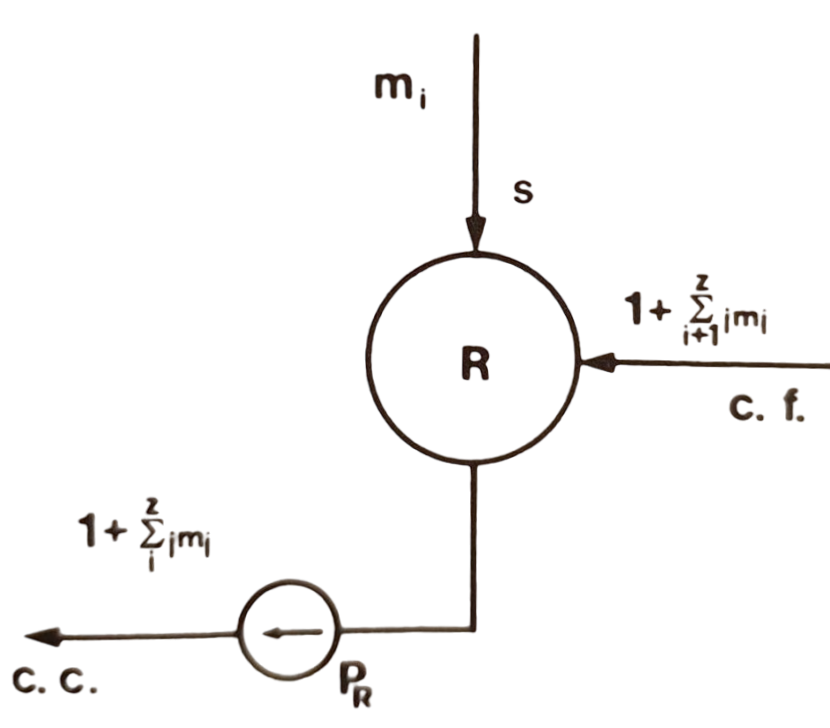
\includegraphics[width=0.3\linewidth]{immagini/miscelatore}
			\label{fig:miscelatore}
		\end{figure}
		
		
		\item \textbf{A superficie}: di tubo in tubo o a fascitubieri.
		
		Non è necessario che i due fluidi si trovino alla stessa pressione.
		
		A valle dello scambiatore è possibile inserire delle valvole di laminazione che permettano di portate il liquido in passaggio di fase alla pressione dello spillamento successivo, oppure si possono usare pompe che elaborino soltanto la portata dello spillamento: entrambe queste alternative sono economicamente abbordabili.
		
		\begin{figure}[H]
			\centering
			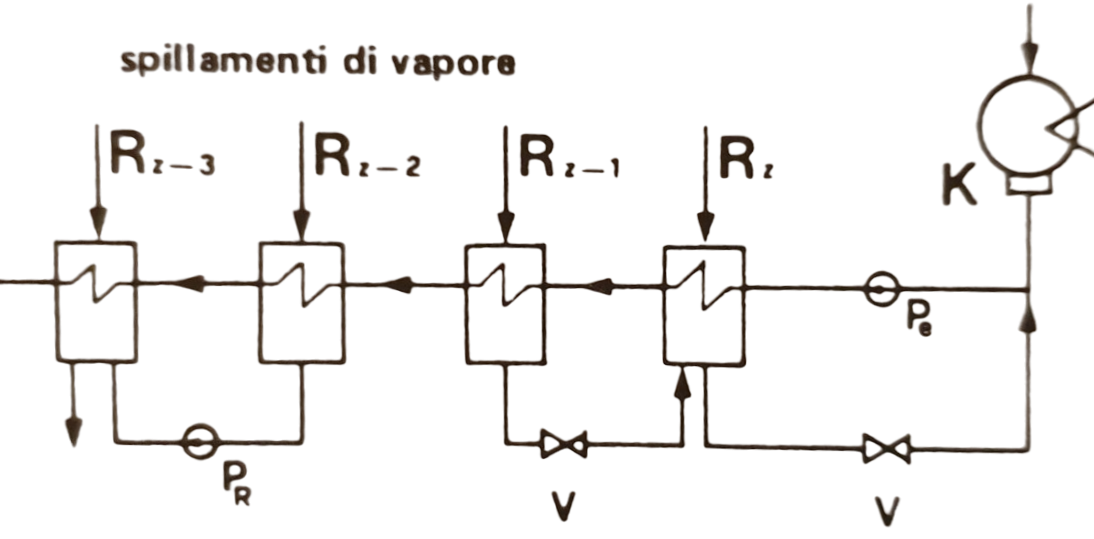
\includegraphics[width=0.5\linewidth]{immagini/rigeneratore}
			\label{fig:rigeneratore}
		\end{figure} 		
	\end{itemize}
	
	Generalmente si adopera un rigeneratore a miscela mentre gli altri rimangono a superficie. 
	
	Il rigeneratore a miscela è sempre presente perché all'interno dell'impianto si raggiungono pressioni sub atmosferiche, ciò significa che potrà entrare dell'aria all'interno delle condotte che andrà in soluzione con l'acqua circolante: i gas disciolti all'interno di un impianto a vapore sono un problema (soprattutto in espansione) perché hanno un comportamento diverso rispetto al vapore; attraverso il degasatore si riesce ad estrarre questi gas dal liquido di lavoro.
	
	Portando l'acqua in condizioni di liquido saturo infatti la solubilità dei gas dispersi nel liquido si annulla ed escono dalla soluzione.
	\begin{figure}[H]
		\centering
		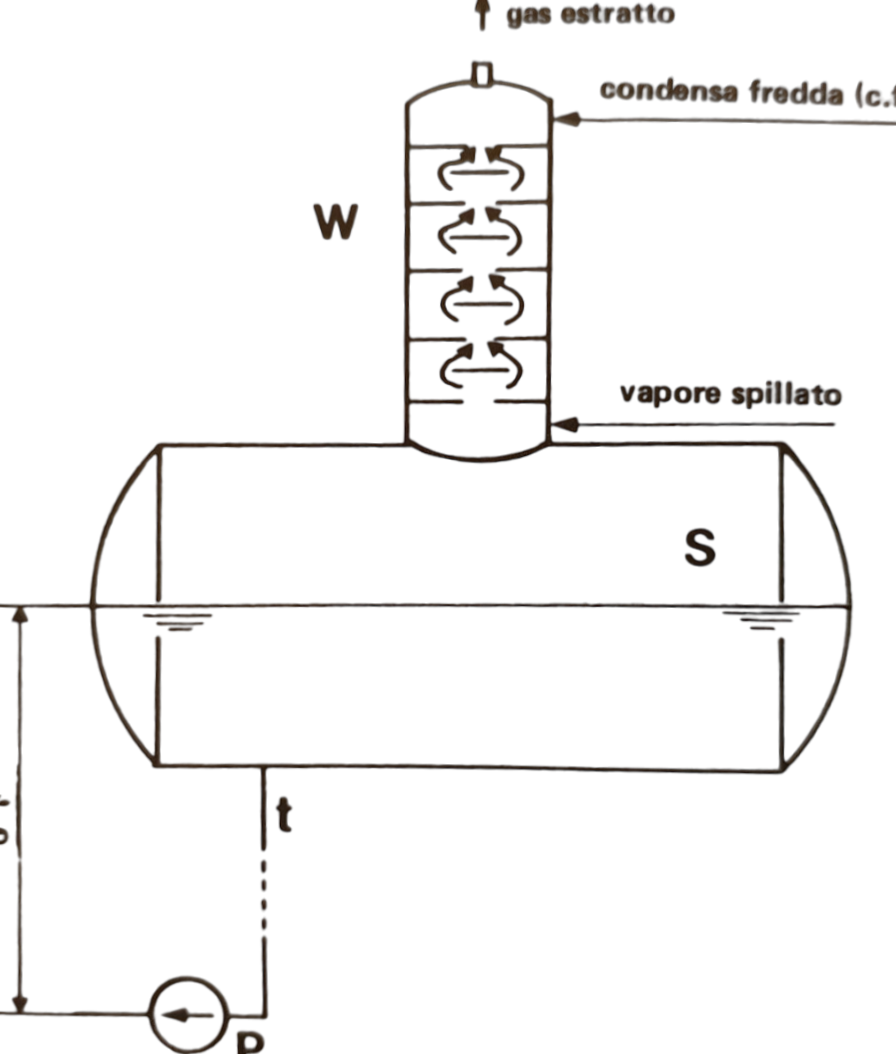
\includegraphics[width=0.4\linewidth]{immagini/degasatore}
		\label{fig:degasatore}
	\end{figure}
	Anche nel condensatore si raggiunge lo stato di liquido saturo, il che potrebbe far pensare di usarlo come degasatore, tuttavia si raggiungono pressioni talmente basse che si dovrebbero usare pompe da vuoto per permettere la separazione dei gas, all'interno del degasatore questo è tranquillamente garantito dalla sovrapressione. \newline 
	
	In ultima analisi, la pompa che estrae il liquido saturo dal degasatore dev'essere posta sottobattente, perché questo è l'unico modo per evitare la cavitazione, infatti dalla classica formula 
	\[NPSH = (P-P_v)-y\]
	La quantità $P-P_v=0$. 	
\end{adjustwidth}


\newpage


\section{Schema impiantistico completo}
	\begin{figure}[H]
		\centering
		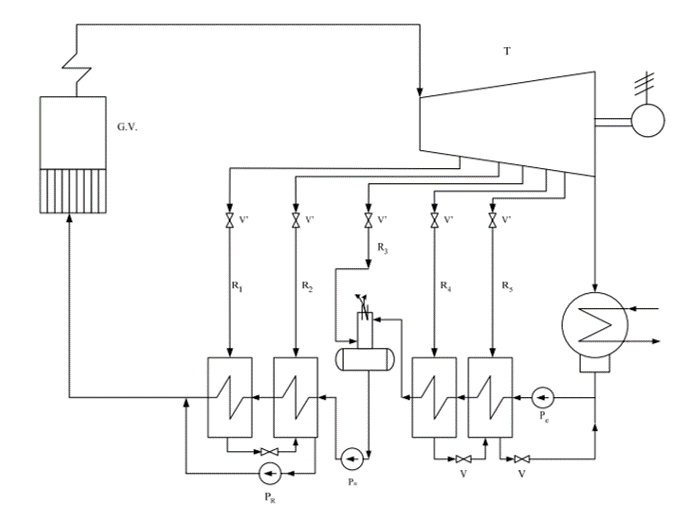
\includegraphics[width=1\linewidth]{immagini/impiantovapore}
		\label{fig:impiantovapore}
	\end{figure}	
\begin{adjustwidth}{2in}{}
	\[R^\text{ott} = {5\over6}\Rightarrow\Delta R^\text{ott} = {1\over6}\]
	La condensa di $R_4,R_5$ viene pompata dalla pompa di estrazione del condensato mentre quella di $R_1, R_2$ dalla pompa $P_R$ e quella di $R_3$ dalla pompa di alimento. 
	
	La  pompa  di  alimento  può essere  azionata,  negli  impianti  più grandi,  mediante uno spillamento di vapore che alimenta una turbopompa di alimento.	
\end{adjustwidth}

\newpage

\section{Elementi di un impianto a vapore}
\begin{figure}[H]
	\centering
	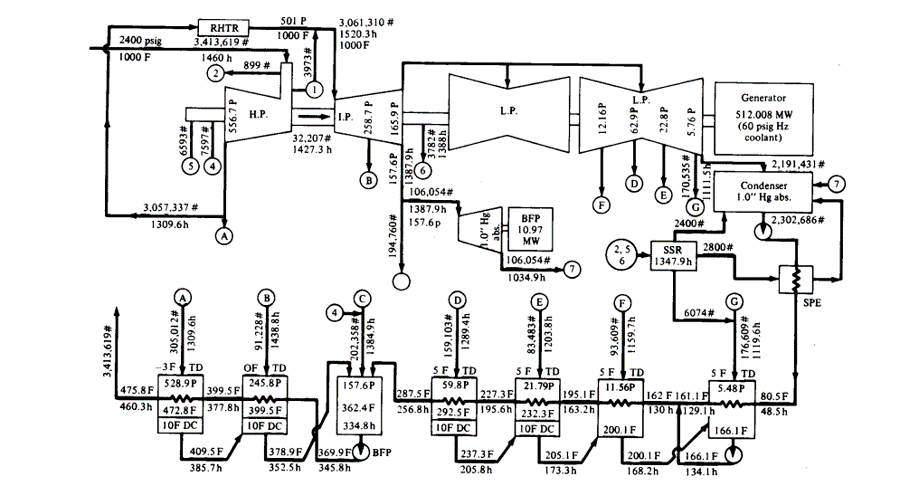
\includegraphics[width=1\linewidth]{immagini/impiantovapore1}
	\label{fig:impiantovapore1}
\end{figure}
\begin{adjustwidth}{2in}{}
	Un impianto reale turbina a vapore presenta una linea di espansione suddivisa in 4 corpi turbina, uno di alta pressione, uno di media pressione e due du bassa pressione a svoluppo speculare, dopodichè è presente una turbina che alimenta tutti gli impianti ausiliari del sistema: tutte le pompe che possono esserci, piuttosto che azionarle con energia elettriva e quindi vincolarle alla frequenza di rete, possono essere alimentate tramite uno spillamento di vapore e quindi avere la libertà di poter variare il numero di giri, e quindi varia la portata elaborata dalle pompe. 
	
	Per quanto riguarda la linea di rigenerazione, qua ci sono  7 rigeneratori di cui uno a miscela ed il rientro delle  condense è semre fatto a pressione più bassa, la condensa viene sempre rimandata al rigeneratore a superficie a pressione più bassa. 
	
	I componenti principali di un impianto a vapore sono

\subsection{Linea di espansione} 
		\begin{figure}[H]
			\centering
			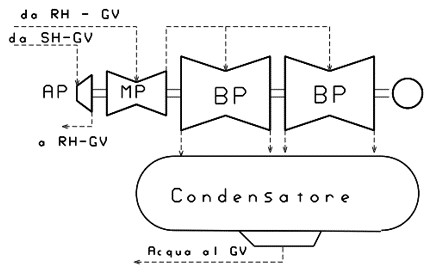
\includegraphics[width=0.3\linewidth]{immagini/impiantovapore2}
			\label{fig:impiantovapore2}
		\end{figure}
		I grandi impianti a vapore, a causa del forte incremento del volume specifico a seguito dell'espansione, presentano più corpi turbina dalle dimensioni via via crescenti. 
\subsection{Turbopompa} che alimenta i sistemi ausiliari
\newpage
\subsection{Scambiatori di calore}
		\begin{itemize}
			\item \textbf{Degasatore}
			\item \textbf{Rigeneratore a superficie} 
			\begin{figure}[H]
				\centering
				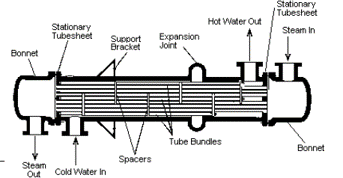
\includegraphics[width=0.5\linewidth]{immagini/rigeneratore1.png}
				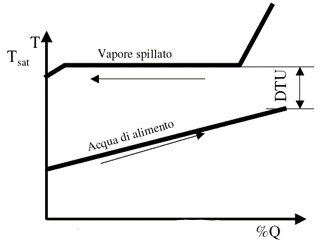
\includegraphics[width=0.3\linewidth]{immagini/rigeneratore2}
				\label{fig:rigeneratore1}
			\end{figure}
			I parametri fondamentali che caratterizzano  la grandezza dello scambiatore per una determinata potenza termica da smaltire sono le differenze di  temperature, prima fra tutte è quella di Pinch Point $\Delta T_{PP}$ che è la minima realizzabile, per cui a pare potenza, ridurre la temperatura di PP consente di aumentare la quantità di calore che viene recuperata ma al tempo stesso comporta un  costo aggiuntivo dovuto all'incremento di superficie dello scambiatore stesso. 
			
			Il vapore spillato si ritrova alla fine dello scambiatore sempre come condensa, per il  repupero di questa condensa si possono percorrere due alternative, o laminare e mandare a pressione inferiore, oppure pompare fino alla pressione superiore. 			
		\end{itemize}
\subsection{Generatore di vapore}
		Il generatore di vapore viene utilizzato per un ampia vastità di impieghi, dalle centrali termoelettriche alla propulsione navale fino alla trazione ferroviaria passando per applicazioni industriali. 
		\begin{figure}[H]
			\centering
			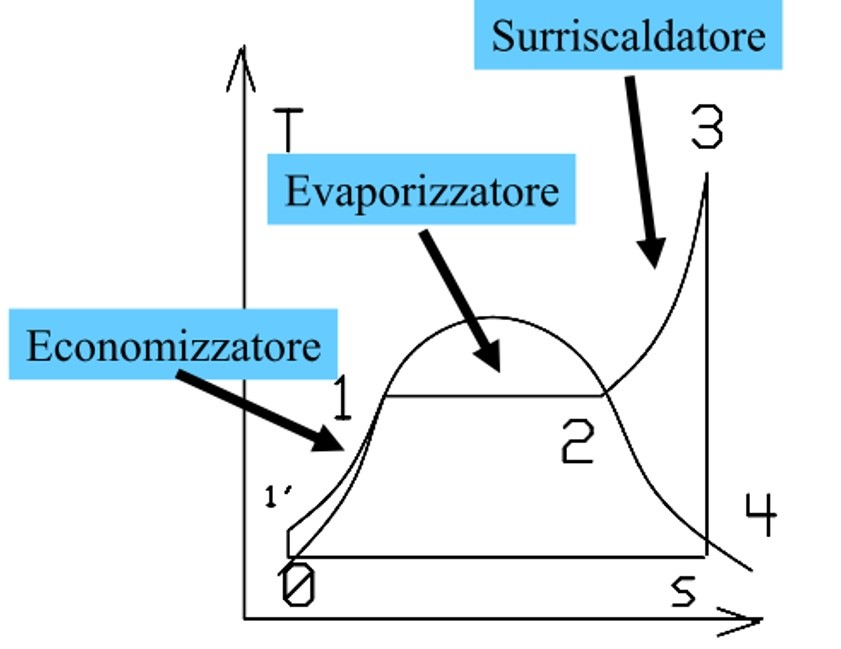
\includegraphics[width=0.3\linewidth]{immagini/impiantovapore3.2}
			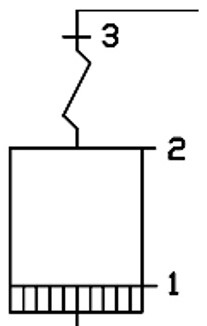
\includegraphics[width=0.1\linewidth]{immagini/impiantovapore3}
			\label{fig:impiantovapore3}
		\end{figure}		
		Le zone della caldaia sono suddivise in base allo stato fisico del fluido:
		\begin{enumerate}
			\item Economizzatore (ECO): stato liquido
			\item Evaporizzatore (EV): Passaggio di fase
			\item Surriscaldatore (SH): stato vapore surriscaldato
			\item Risurriscaldatore (RH): stato vapore surriscaldato
		\end{enumerate}  
\newpage
		si sono 3 principali tipi di generatori di vapore

\subsubsection{Caldaie a grande corpo} 
\subsubsection{Caldaie a tubi di fumo}
			\begin{figure}[H]
				\centering
				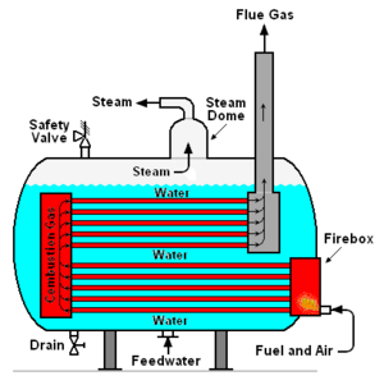
\includegraphics[width=0.3\linewidth]{immagini/GeneratoreVapore}
				\label{fig:generatorevapore}
			\end{figure}
			
			Un involucro contiene l'acqua scaldata da tubi al cui interno passano i prodotti della combustione
\subsubsection{Caldaie a tubi d'acqua}
			\begin{figure}[H]
				\centering
				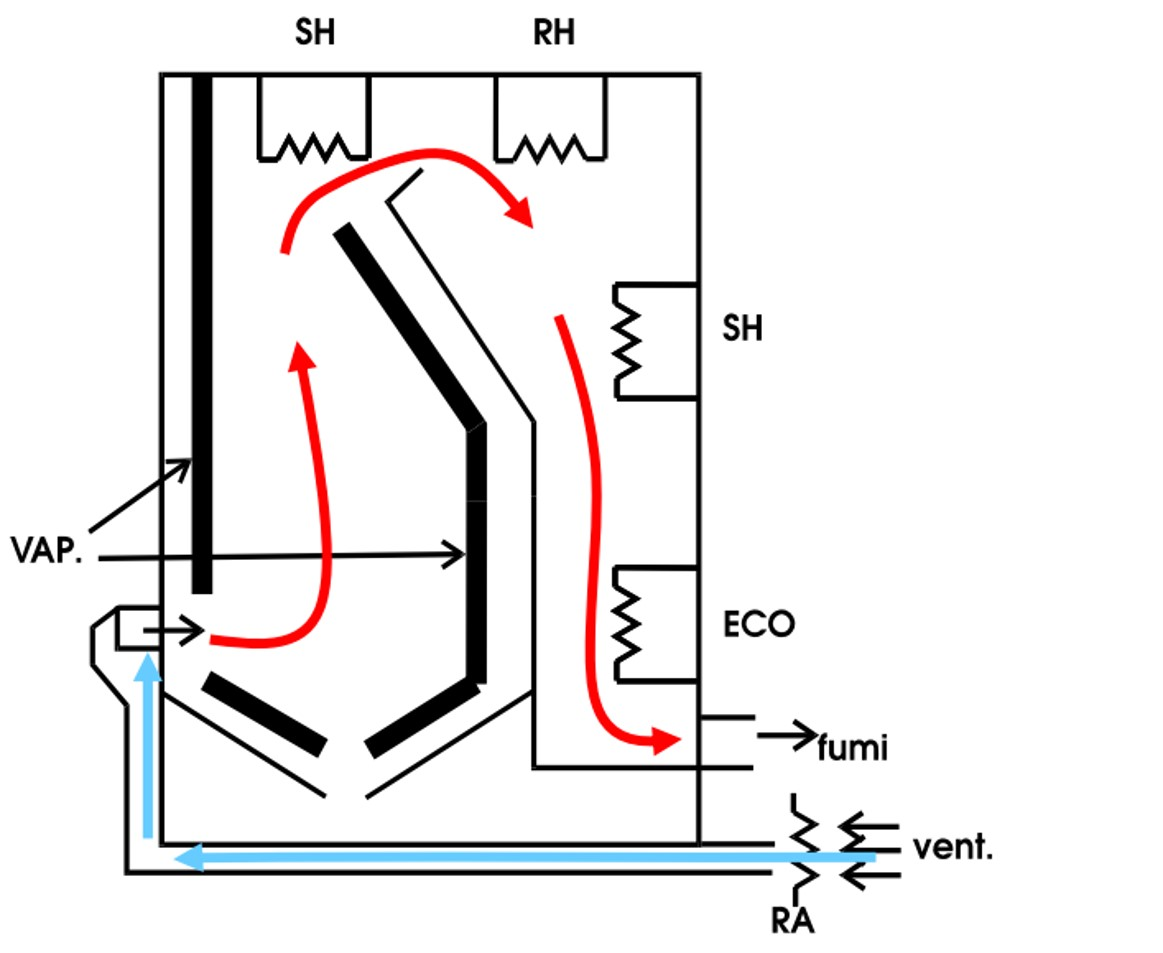
\includegraphics[width=0.5\linewidth]{immagini/Immagine12}
				\label{fig:immagine12}
			\end{figure}			
			Nell'ambiente principale si sviluppa il circuito aria-fumi mentre l'acqua 
			
			Qual è il senso della disposizione degli elementi della caldaia? 
		
			Cosa incontrano i fumi? 
			\begin{figure}[H]
				\centering
				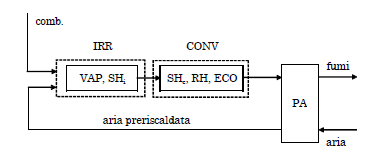
\includegraphics[width=0.5\linewidth]{immagini/GeneratoreVapore1}
				\label{fig:generatorevapore1}
			\end{figure}
			Questi dapprima incontrano la zona irraggiata composta dal vaporizzatore e da un primo surriscaldatore irraggiato e poi incontrano la zona convettiva, composta dal surriscaldatore convettivo, l'eventuale risurriscaldatore e poi l'economizzatore. \newline 
			
			L'acqua, se dovesse seguire il percorso dei fumi, presenterebbe un andamento simile 
			
			DISEGNO DIAGRAMMA TQ "sbagliato"
			
			E non è affatto la situazione ottimale perché se l'obiettivo è quello di minimizzare la differenza di temperatura media, si cerca un andamento del genere
			
			DISEGNO DIAGRAMMA TQ "giusto"
			
			L'acqua allora segue un percorso diverso.
			\begin{figure}[H]
				\centering
				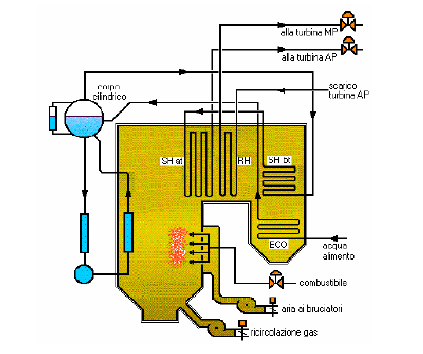
\includegraphics[width=0.6\linewidth]{immagini/GeneratoreVapore2}
				\label{fig:generatorevapore2}
			\end{figure}
			All'interno dei tubi è convogliata all'economizzatore, poi verso il corpo cilindrico all'interno del vaporizzatore, e poi ai relativi surriscaldatori. \newline 
			
			Il motivo di questa disposizione dei circuiti di aria e dei fumi ha una motivazione tecnologica, di resistenza dei materiali
			\begin{figure}[H]
				\centering
				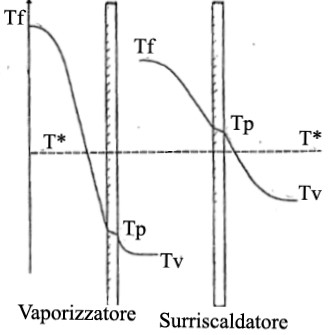
\includegraphics[width=0.3\linewidth]{immagini/GeneratoreVapore3}
				\label{fig:generatorevapore3}
			\end{figure}
			Siano $T_f, T_v, T_P$ le temperature rispettivamente dei fumi, del vapore e della parete, e $T^*$ la temperatura di resistenza del materiale del tubo. 
			
			Si pone il vaporizzatore nella zona più a temperatura più alta perché il coefficiente di scambio termico del vapore in passaggio di fase è 1o volte maggiore del coefficiente di scambio termico del vapore surriscaldato;
			e ciò consente di avere sulla parete una temperatura inferiore a quella di resistenza del materiale. 
			
			Infatti dal fatto che il calore che fluisce dev'essere costante
			\[Q = hS\Delta T\]
			Allora $h\gg\Rightarrow\Delta T\ll$ e la maggior parte del salto di temperatura viene eseguito lato fumi. 
			
			Se questa disposizione non fosse rispettata, si avrebbero da una parte sempre i fumi mentre dall'altra vapore surriscaldato e i due coefficienti di scambio termico si equivarrebbero e questo comporterebbe una temperatura all'interfaccia maggiore di quella di resistenza del materiale. 			
			
			Si pone il vaporizzatore nella parte a temperatura più alta, dove c'è sia irraggiamento che convezione; il profilo di temperatura si disegna partendo da una temperatura dei fumi molto maggiore di quella di resistenza del materiale. 
			
			Quindi per mettere il surriscaldatore è necessario aspettare che la temperatura dei fumi si sia abbassata e si sarà certi che la temperatura di parete sarà al di sotto di quella di resistenza del materiale. 
			 						
			\subsubsection{Circuito Aria-Fumi}
			Sono possibili due soluzioni differenti:
			\begin{itemize}
				\item A caldaia pressurizzata se un solo ventilatore è posto all'ingresso del circuito.
				\item A tiraggio bilanciato se vi sono due ventilatori, uno all'ingresso e uno in uscita. \\
				Questa soluzione consente una movimentazione dell'aria  e dei fumi più efficace ma anche un onere aggiuntivo dovuto alla compressione dei fumi caldi in uscita che richiederanno un lavoro specifico maggiore dell'aria fredda che può essere spinta in ingresso. 
				\item Il preriscaldatore di tipo \textit{Ljungström} è importante perchè consente di aumentare  l'eficienza del generatore di vapore in quanto consente di preriscaldare  l'aria in ingresso a discapito dei fumi in uscita. 
				
				La presenza di questo preriscaldatore è tanto più importate quanto più è alto i grado dirigenerazione, perchè  ad un grado di rigenerazione più alto corrisponde un'ingresso dell'acqua all'economizzatore a temepratura più elevata e quindi presumibilimente  dall'altro lato usciranno dei fumi a temepratura più elevata, quindi per abbassare  la temperatura dei fumi e quindi aumentare l'efficienza del generatore di vapore si usa questo preriscaldatore. 
				
				Dato che i due flussi non possono essere miscelati e il coefficiente convettivo degli stessi risulta modesto (si parla senza perdite di generalità di uno scambio termico aria-aria) questo sistema sfrutta l'elevata capacità termica del materiale col quale è costituito (solitamente materiali ceramici), questo recuperatore è formato da un cilindro di grandi dimensioni rotante attorno al proprio asse. Esso contiene pacchi di lamierini che, per effetto della rotazione del mantello cilindrico, vengono investiti dai fumi caldi e successivamente dall'aria fredda alla quale cedono il calore che hanno immagazzinato dai fumi. 
				\begin{figure}[H]
					\centering
					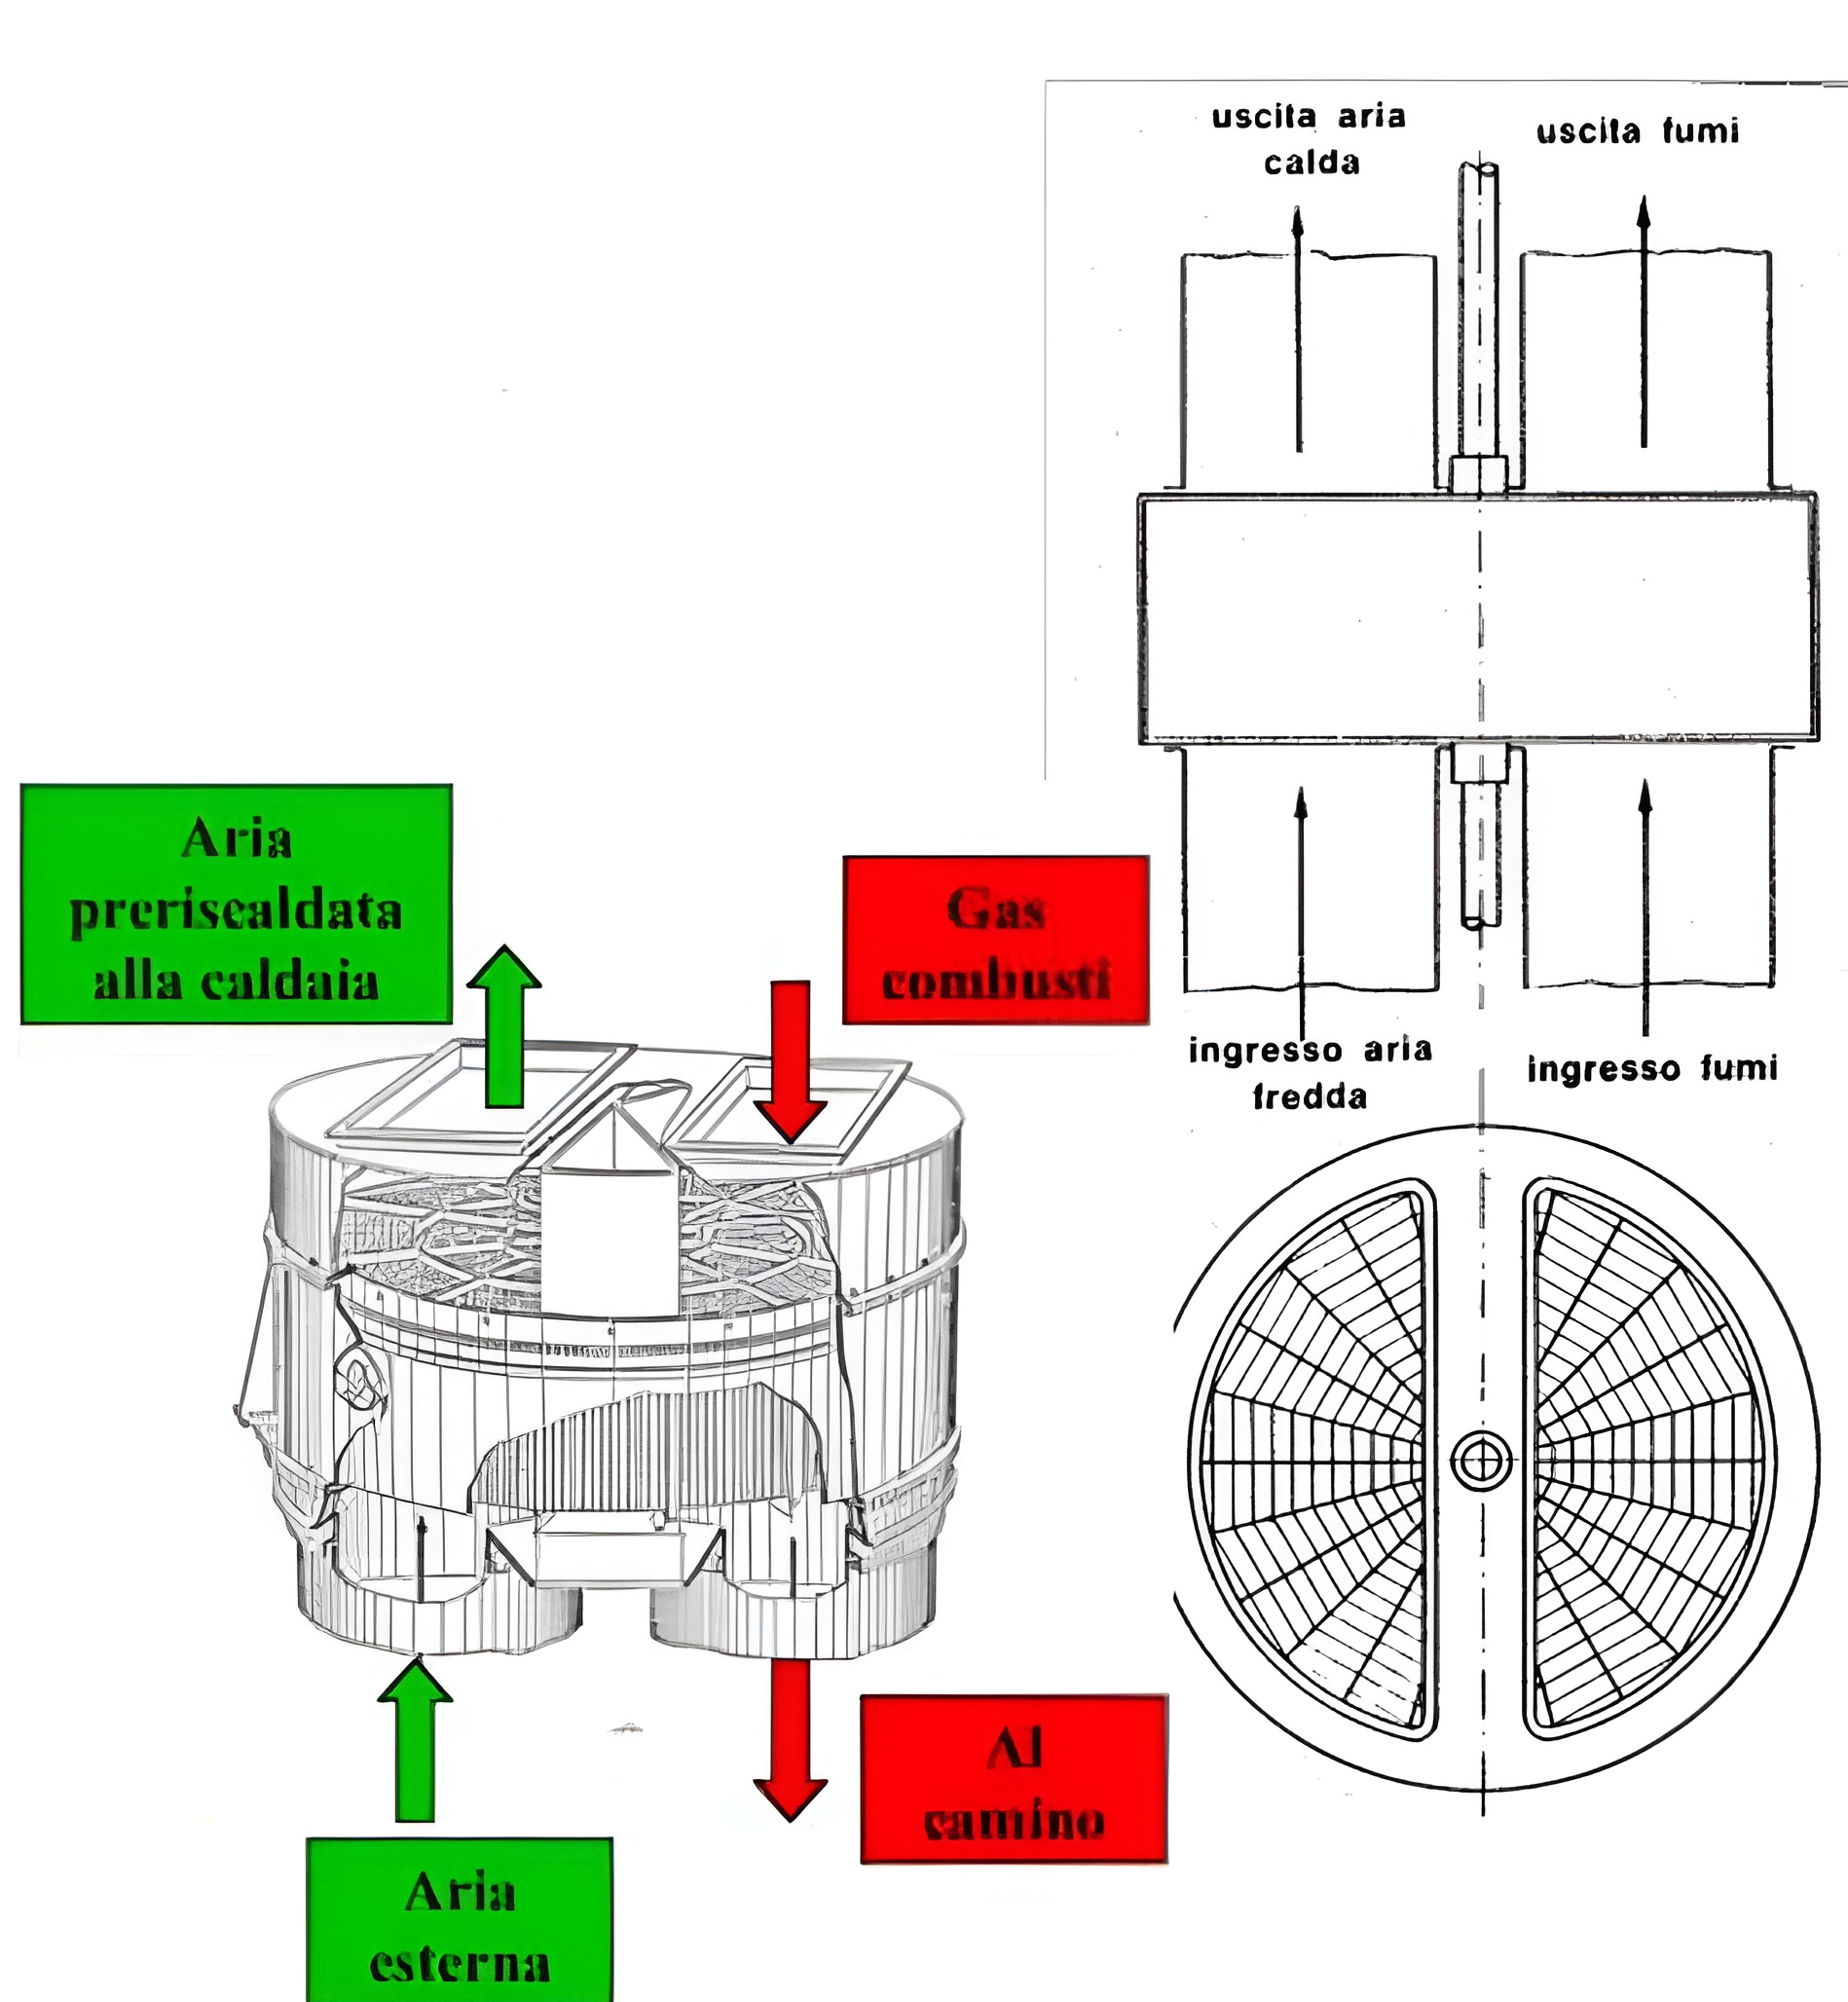
\includegraphics[width=0.3\linewidth]{immagini/Immagine14}
					\label{fig:immagine14}
				\end{figure}
								
				\item Il recuperatore a superficie, a piastre è un'altra soluzione percorribile in alternativa al \textit{Ljungström}, si utilizzano per impianti più piccoli perché per impianti di notevoli dimensioni richiederebbero un ingombro troppo elevato.
			\end{itemize}
			
			\subsubsection{Circuito Acqua-Vapore}
			Ormai è più che noto che il circuito acqua-vapore si suddivida in diversi elementi come economizzatore (costituito da fasci tubieri alettati), evaporatore, surriscaldatore e risurriscaldatore, questi - come visto - suddivisi tra loro perché le caratteristiche fisiche del fluido  all'interno di ogni singolo elemento sono diverse. 
			
			Si è già visto che l'evaporatore, avendo un coefficiente di scambio termico molto maggiore rispetto al surriscaldatore, viene messo a contatto  coi fumi nella parte più calda del generatore di vapore.\newline
			
			Fin'ora però dalla trattazione ci si è dimenticati di menzionare un componente di vitale importanza per il generatore di vapore: il \textbf{Corpo Cilindrico}. 
			
			Questo è un contenitore che riceve in input la miscela acqua-vapore in uscita dall'evaporatore e il liquido saturo in uscita dall'economizzatore e per gravità separa la fase liquida dalla fase vapore, a questo punto pescando da basso si ritrova liquido da mandare all'evaporatore e pescando dall'alto si prende il vapore da mandare al surriscaldatore.
			
			Inoltre il corpo cilindrico assolve anche un'importante funzione "polmone", ovvero di regolazione di portata di vapore in caso ce ne fossero fluttuazioni. \newline
			
			Importante specificare che il corpo cilindrico ha senso d'esistere solamente per pressioni subcritiche, per pressioni supercritiche infatti, non essendoci differenza di densità tra fase liquida e fase vapore, il corpo cilindrico viene sostituito da un altro fascio tubiero, questo tuttavia  comporta la necessità di inserimento di una pompa che faccia circolare il fluido all'interno dell'evaporatore. 
			
			\subsubsection{Tipi di circolazione}
			\begin{itemize}
				\item \textbf{Circolazione naturale}\\
				In una configurazione subcritica, quindi con corpo cilindrico, è possibile sfruttare il cosiddetto "effetto termosifone": la  forza  fluidomotrice è assicurata  dalla  differenza  di pressione  idrostatica,  legata  alla spinta di galleggiamento. 
				
				Man mano che l'acqua riceve calore, avrà una percentuale di vapore sempre maggiore, e quindi questo diminuirà  la densità media e si produrrà la spinta che  fa salire l'acqua che si scalda e mantiene in movimento il circuito dell'evaporatore. 
				
				\item \textbf{Circolazione assistita}\\
				La differenza di densità tra vapore e liquido saturo si riduce mano a mano che ci si avvicina (per poi annullarsi) alle condizioni critiche, ciò comporta che anche i dei generatori di vapore subcritici, nonostante la circolazione sia garantita dall'effetto "termosifone", è necessario installare una pompa che aiuti il fluido in questo attraversamento. 
				
				I tubi dei vari componenti del generatore di vapore sono posti verticalmente.  
				
				\item \textbf{Circolazione forzata}\\
				Una volta arrivati alla pressione critica non esiste più differenza di densità tra vapore e liquidi e quindi si passa ad una configurazione di circolazione forzata: sparisce il corpo cilindrico ed il sistema è tutto alimentato tramite una pompa.
				
				Il generatore di vapore avrà caratteristiche totalmente differenti da quanto visto fin'ora che decretano costi di vapore più elevati. 
			\end{itemize}			
\end{adjustwidth}

\newpage
\part{Impianti combinati}
\begin{adjustwidth}{2in}{}
	Un ciclo combinato è l'unione delle tecnologie viste fin'ora. 
	
	l'idea di base è che in un gruppo turbogas moderno si riescono a raggiungere temperature massime molto elevate e ciò comporta avere fumi in uscita dall'espansione ancora a temperature elevate (ma a basse pressioni) che possono essere utilizzati, non per la produzione di lavoro, ma per il recupero di calore. 
	
	Si cerca così di valorizzare il contenuto entalpico dei fumi per via termica, convogliando i fumi in un generatore di vapore a recupero che permetta di riscaldare l'acqua di un impianto a vapore. 
	
	In questo modo il ciclo turbogas viene denominato ciclo Topping mentre quello a vapore ciclo Bottoming.  \newline 
	
	Il ciclo combinato presenta molti aspetti positivi
	\begin{itemize}
		\item Rendimento elevato: si immette combustibile soltanto all'interno del ciclo turbogas mentre si produce lavoro sia col turbogas che col vapore
		\item Basso costo: non è necessario un vero e proprio generatore di vapore, mentre la turbina a vapore non raggiunge pressioni elevatissime 
		\item Emissioni contenute: gli unici prodotti della combustione provengono dal ciclo turbogas
	\end{itemize}
\begin{figure}[H]
	\centering
	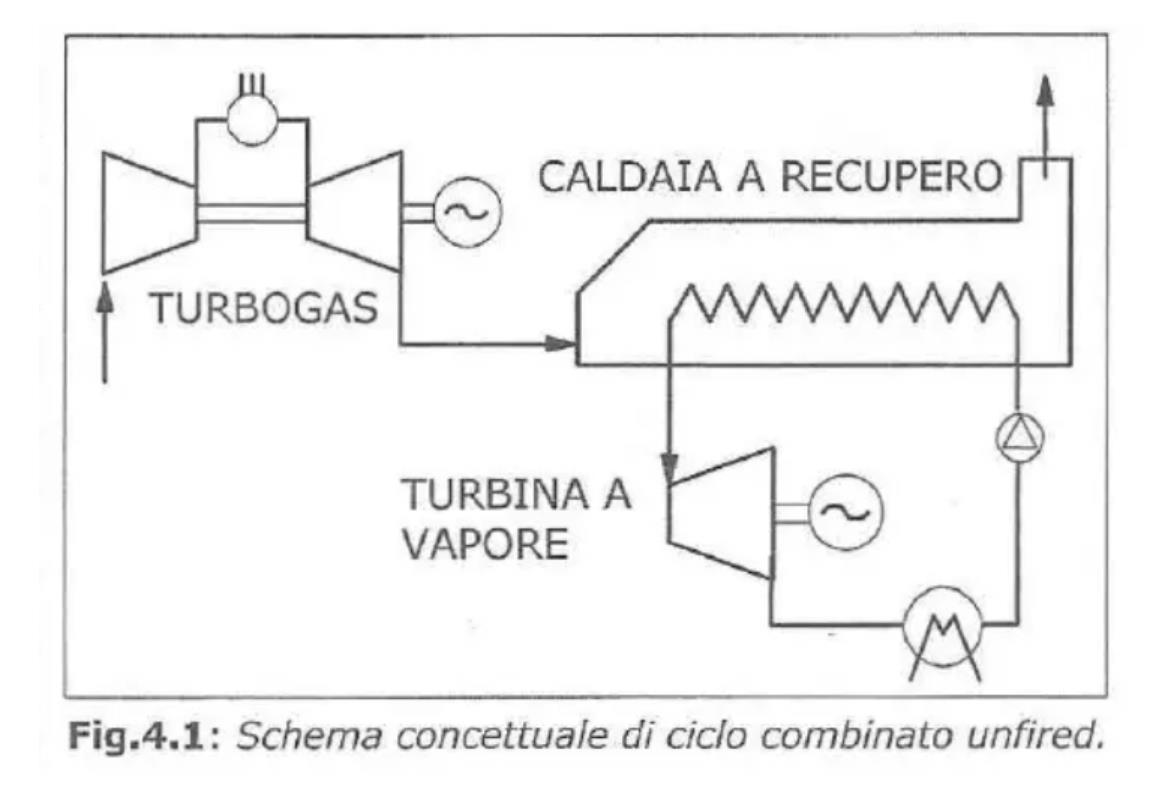
\includegraphics[width=0.5\linewidth]{immagini/impianticombinati}
	\label{fig:impianticombinati}
\end{figure}
	I cicli combinati possono essere 
	\begin{itemize}
		\item \textbf{Mixed}: a ciclo misto, aria viene miscelata a vapore 
		\item \textbf{Unmixed}: se i due fluidi non vengono mai a contatto diretto
		\item \textbf{Unfired}: se non vi è postcombustione dei fumi
		\item \textbf{Fired}: se vie è postcombustione dei fumi.
		
		Questi infatti contenendo una grande quantità di ossigeno, se miscelati con un combustibile possono dar luogo ad una combustione.
		\item \textbf{Green Field}: se vengono sviluppati ex novo con l'intento di costruire da zero un impianto combinato
		\item \textbf{Repowering}: se si adattano impianti preesistenti al ciclo combinato
	\end{itemize}
\end{adjustwidth}




\section{Analisi termodinamica}
\begin{adjustwidth}{2in}{}
	\begin{figure}[H]
		\centering
		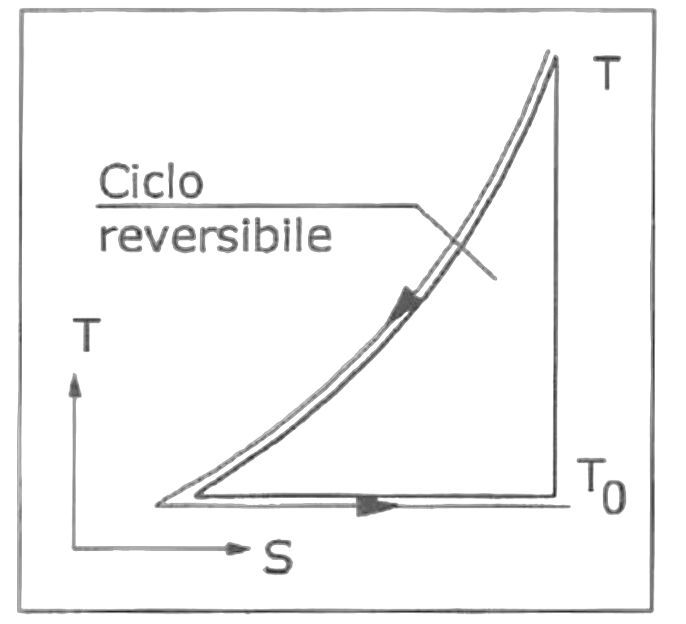
\includegraphics[width=0.5\linewidth]{immagini/impianticombinati1}
		\label{fig:impianticombinati1}
	\end{figure}
	Si sottopone ai gas in raffreddamento un ciclo termodinamico reversibile che massimizza il lavoro estraibile dalla sorgente termica di recupero. \newline 
	
	Si introduce una nuova funzione di stato, l'Energia libera di Gibbs
	\[\Delta G = h-Ts\]
	Questa oltre a individuare se una reazione avverrà spontaneamente o meno, darà indicazioni sulla possibilità di estrarre lavoro, infatti si può scrivere 
	\[\begin{split}
		L_\text{rev} & = \dot{m}[(h-T_0s)-(h_0-T_0s_0)] = \dot{m}(\Delta h - T_0\Delta s) \\ & = \dot{m}\Delta h \left(1-T_0\dfrac{\Delta s}{\Delta h}\right) = Q_{av}\left(1-T_0\dfrac{\Delta s}{\Delta h}\right)
	\end{split}\]
	Dove con $Q_{av}$ si è individuata la potenza termica disponibile, ovvero tutto il calore che sarebbe possibile recuperare raffreddando fino a $T_0$ i fumi. \newline 
	
	Per un gas ideale $c_P=cost$ e allora si può scrivere 
	\[L_\text{rev} = Q_{av}\left(1-\dfrac{T_0}{TML}\right) \qquad \eta_\text{rev} = \left(1-\dfrac{T_0}{TML}\right)\] 
	Dove $TML$ è la temperatura media logaritmica. \newline 
	
	Si definiscono i rendimenti di primo principio e di secondo principio come 
	\[\eta_I = \dfrac{L}{Q_{av}} = \dfrac{L}{Q_1}\dfrac{Q_1}{Q_{av}} = \eta_{th}\chi\]
	Dove $\chi$ è il fattore di recupero del calore.
	\[\eta_{II} = \dfrac{L}{L_\text{rev}} \] 
	In modo che 
	\[\eta_I = \eta_{II}L_\text{rev}\]
	Sebbene non ci si addentri in specifiche definizioni, il concetto principale che deve rimanere è che il ciclo combinato deve massimizzare due effetti per poter essere efficace:$\eta_{th}$ e $\chi$. 
	
	Per il ciclo visto a inizio paragrafo vale tranquillamente $\chi=1$, purtroppo realizzare nella pratica tale ciclo ideale è impossibile perché non esiste fluido che sia in grado di comportarsi allo stesso tempo come un gas nella fase di assorbimento di calore e come un vapore condensate.\newline 
	
	Nell'analisi per individuare il miglior ciclo sottoposto si parte ovviamente da quello di Carnot.
	\begin{figure}[H]
		\centering
		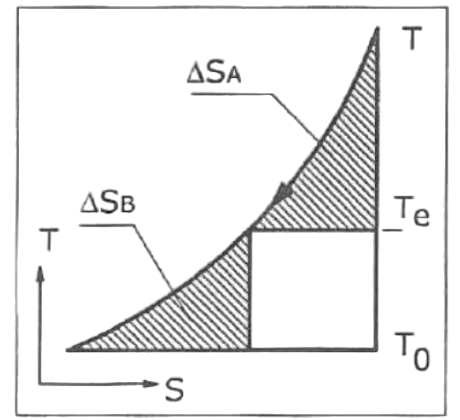
\includegraphics[width=0.5\linewidth]{immagini/impianticombinati3}
		\label{fig:impianticombinati3}
	\end{figure}
	Il calore viene recuperato da $T_0$ a $T_e$ e si individuano due fattori di perdita
	\begin{itemize}
		\item $\Delta S_A$ di cessione causato dallo scambio termico tra gas e fluido ad una determinata $\Delta T$.
		\item $\Delta S_B$ di assorbimento causato dal mancato raffreddamento del gas fino alla $T_0$: tutte le temperature inferiori a $T_e$ non permettono di recuperare il calore.
	\end{itemize}
	Grazie al ciclo di Carnot sottoposto si possono studiare principalmente due casi limite. \newline 
	
	\textbf{Caso limite 1}
	\[
		T_e = T \Rightarrow \begin{cases}
			\eta_{th} = \max\quad\text{Si alza al massimo la temperatura massima} \\
			\xi = 0 \quad\text{non viene recuperato in alcun modo il calore}
		\end{cases}
	\]
	\textbf{Caso limite 2}
	\[
	T_e = T_0 \Rightarrow \begin{cases}
		\eta_{th} = \min \\
		\xi = \max \quad\text{si recupera tutto il calore}
	\end{cases}
	\]
	Tra i casi limite, esiste un valore ottimale?
	
	Dalle definizioni 
	\[\begin{dcases}
		\Delta S_A = c_P\dfrac{T-T_e}{T_e} - c_P\ln\left(\dfrac{T}{T_e}\right) \\
		\Delta S_B = c_P\dfrac{T_e-T_0}{T_0} - c_P\ln\left(\dfrac{T_e}{T_0}\right)
	\end{dcases}\]
	Per massimizzare il rendimento si impone che la somma di questi due elementi sia la minima
	\[\Sigma = \Delta S_A + \Delta S_B = c_P\left[\dfrac{T}{T_e} - 1 + \dfrac{T_e}{T_0} - 1 - \ln\left(\dfrac{T}{T_e}\dfrac{T_e}{T_0}\right)\right]\]
	Volendo ottimizzare il $T_e$ si impone 
	\[\dfrac{d\Sigma}{dT_e} = 0 \Leftrightarrow T_e = \sqrt{TT_0}\]
	Ed il fattore di recupero diventa così esprimibile come 
	\[\chi = \dfrac{T-T_e}{T-T_0}\]
	Ora che si conosce un valore ottimale di temperatura massima raggiungibile dal ciclo sottoposto, quali alternative si possono vagliare rispetto al ciclo di Carnot? 
	\begin{itemize}
		\item \textbf{Passaggi di fase a più livelli di pressione}
		\begin{figure}[H]
			\centering
			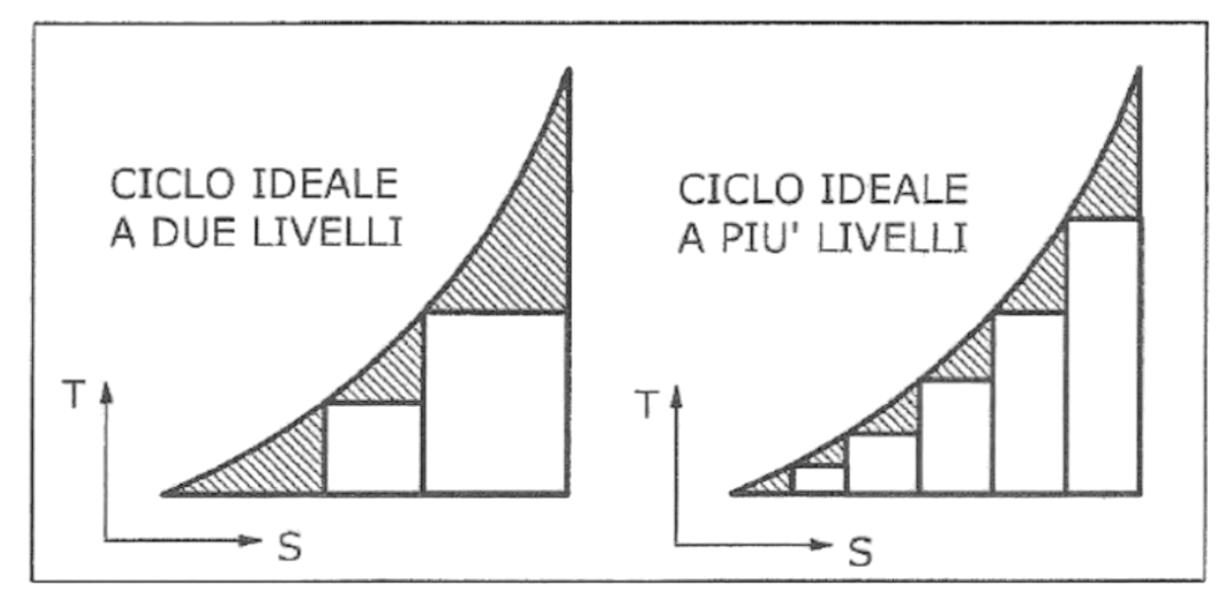
\includegraphics[width=0.5\linewidth]{immagini/impianticombinati4}
			\label{fig:impianticombinati4}
		\end{figure}
		\item \textbf{Impianto a vapore ipercritico}
		\begin{figure}[H]
			\centering
			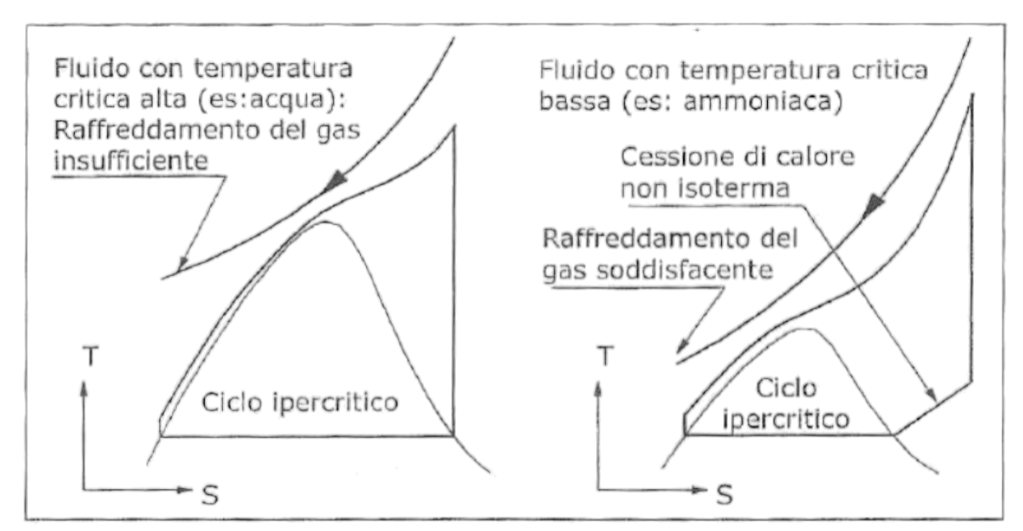
\includegraphics[width=0.5\linewidth]{immagini/impianticombinati5}
			\label{fig:impianticombinati5}
		\end{figure}
		\item \textbf{Compressione interregriferata}
		\begin{figure}[H]
			\centering
			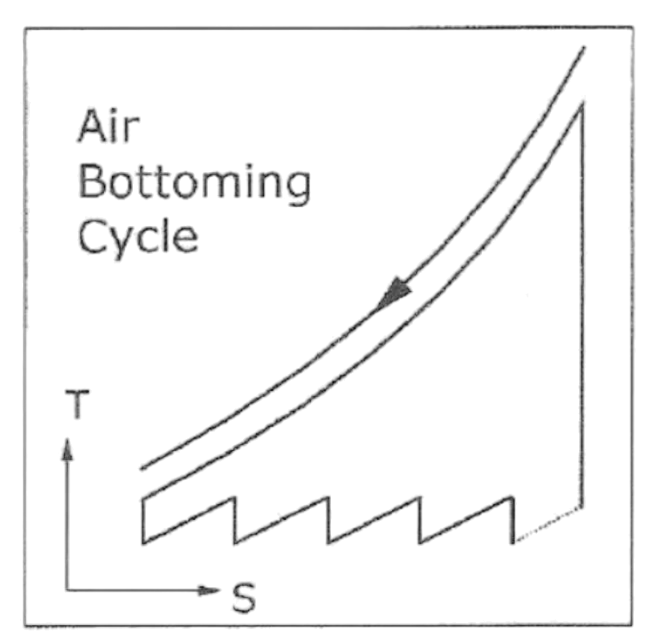
\includegraphics[width=0.3\linewidth]{immagini/impianticombinati6}\
			\label{fig:impianticombinati6}
		\end{figure}
		\newpage
		\item \textbf{Ciclo a vapore con surriscaldamento}
		\begin{figure}[H]
			\centering
			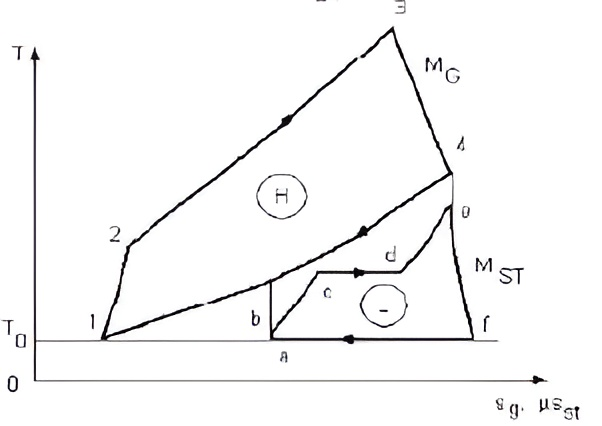
\includegraphics[width=0.5\linewidth]{immagini/impianticombinati7}
			\label{fig:impianticombinati7}
		\end{figure}
		Nonostante la vaporizzazione abbia pendenza costante, tuttavia grazie alla trasformazione all'interno dell'economizzatore e a quella all'interno del surriscaldatore, le due entropie $\Delta S_A$ e $\Delta S_B$ risultano opportunamente scalate, in questo modo si riesce ad aumentare sia $\chi$ che $\eta$ perché aumentano sia calore che temperatura massima del ciclo. 
		
		l'ideale sarebbe eseguire lo stesso ciclo a più livelli di pressione.
	\end{itemize}
	Il rendimento del ciclo combinato sarà 
	\[\eta_{cc} = \eta_{TG} + (1-\eta_{TG}-\chi)\eta_I\approx0.6\]
	È come se si valorizzasse doppiamente il combustibile all'interno del ciclo turbogas. \newline
	
	Ha senso rigenerare?
	
	Il calore del ciclo combinato è già in fase di recupero, così facendo si diminuisce l'effetto di molteplicità delle sorgenti intrinsecamente al ciclo.	
\end{adjustwidth}


\newpage


\section{Generatore di vapore a recupero}
\begin{adjustwidth}{2in}{}
	Il generatore di vapore a recupero si compone delle spesse parti del generatore di vapore classico, cioè economizzatore, surriscaldatore e vaporizzatore, ma questa volta sono posti tutti controcorrente perché non esiste più il problema della resistenza del materiale.
\begin{figure}[H]
	\centering
	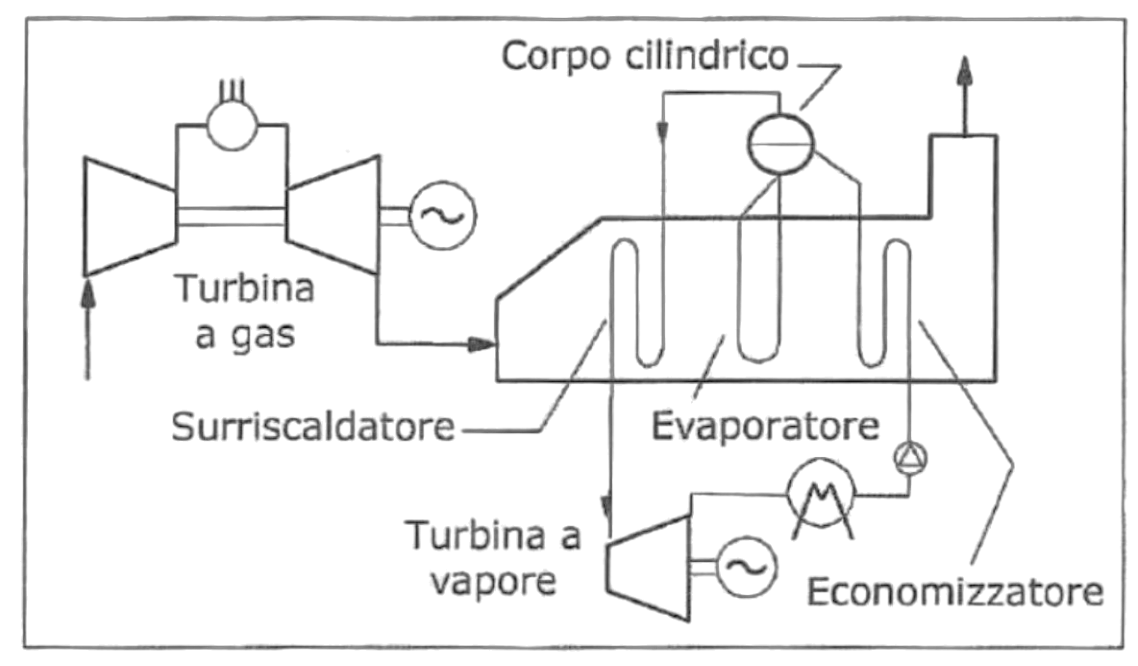
\includegraphics[width=0.5\linewidth]{immagini/impianticombinati8}
	\label{fig:impianticombinati8}
\end{figure}
	All'interno del generatore di vapore a recupero, per acqua e fumi si possono individuare i seguenti andamenti	
\begin{figure}[H]
	\centering
	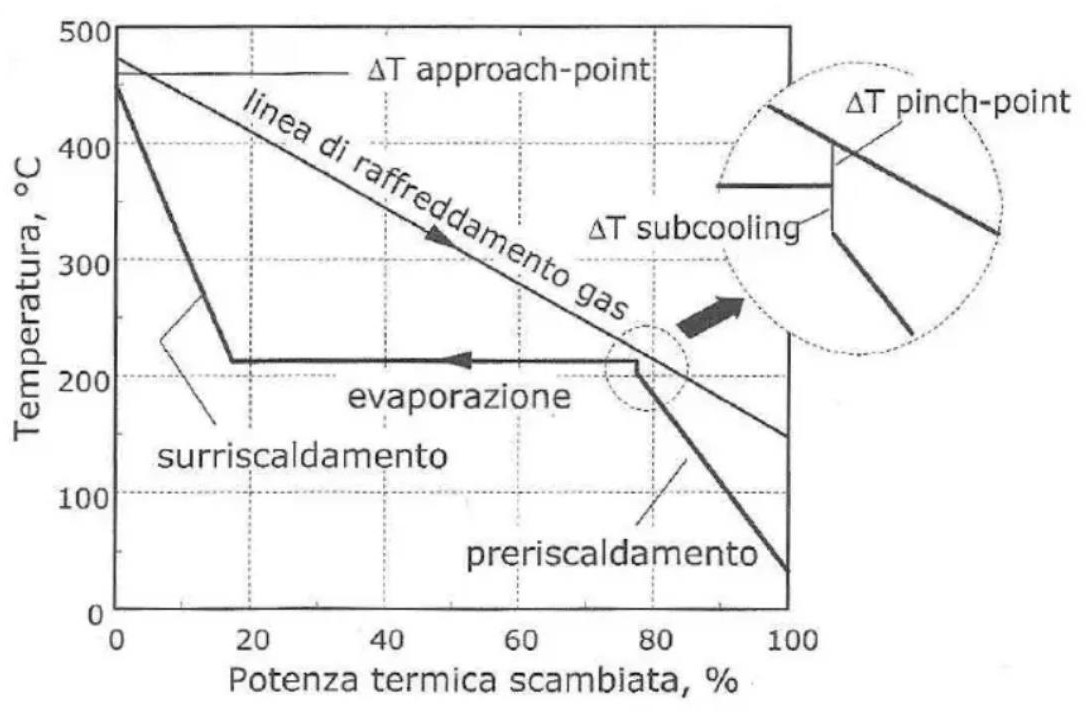
\includegraphics[width=0.7\linewidth]{immagini/impianticombinati9}
	\label{fig:impianticombinati9}
\end{figure}
	Il $\Delta T$ di subcooling (sottoraffreddamento) è necessario perché essendo il liquido più voluminoso del vapore, il passaggio di fase comporterebbe una sostanziale interferenza col regime di moto nei tubi, in questo modo si eliminano i rischi di evaporazione prematura nei fasci tubieri dell'economizzatore. 
\end{adjustwidth}



\subsection{GVR a più livelli di pressione}
\begin{adjustwidth}{2in}{}
	\begin{figure}[H]
		\centering
		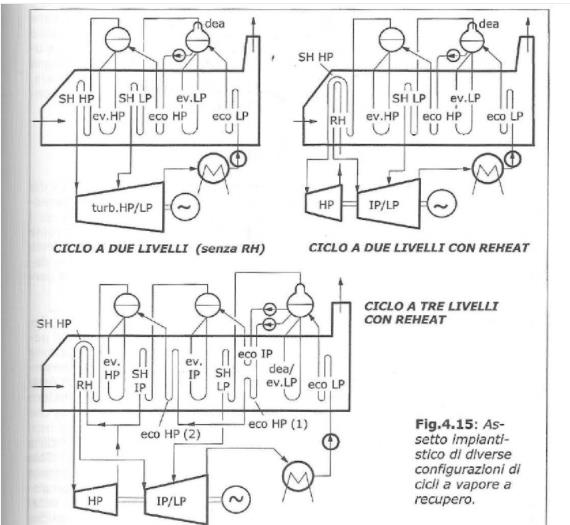
\includegraphics[width=0.8\linewidth]{immagini/impianticombinati10}
		\label{fig:impianticombinati10}
	\end{figure}
	L'obiettivo è quello di minimizzare la temperatura tra gas e liquido che si sta surriscaldando. \newline 
	
	In parallelo ai banchi del surriscaldatore di alta pressione può essere inserito un risurriscaldatore: hanno temperature simili e incontrano i gas caldi praticamente nella stessa posizione.
	\begin{figure}[H]
		\centering
		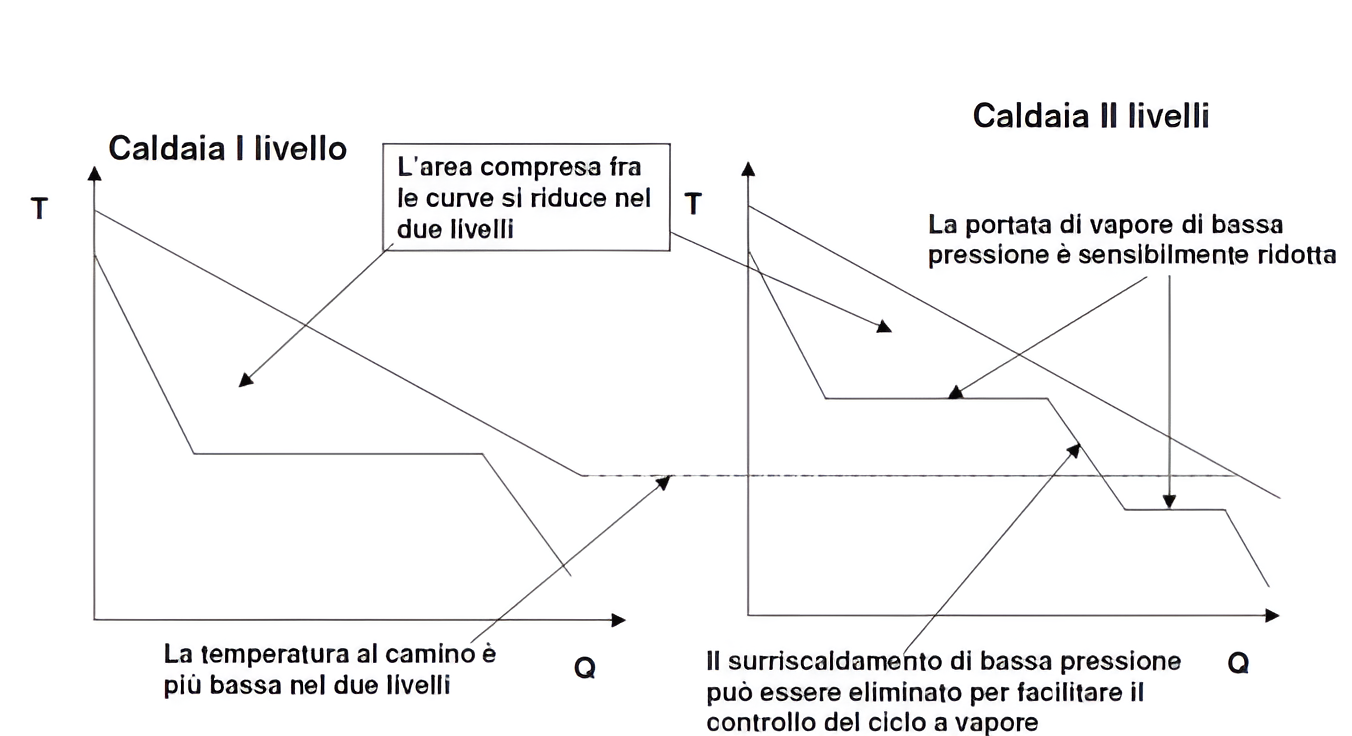
\includegraphics[width=0.8\linewidth]{immagini/impianticombinati11}
		\label{fig:impianticombinati11}
	\end{figure}	
\end{adjustwidth}

\newpage

\section{Variazioni impiantistiche}
\subsection{Ciclo Fired}
\begin{adjustwidth}{2in}{}	
\begin{figure}[H]
	\centering
	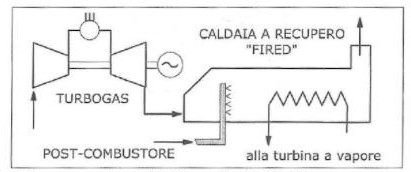
\includegraphics[width=0.5\linewidth]{immagini/impianticombinati12}
	\label{fig:impianticombinati12}
\end{figure}
	Attraverso il ciclo fired si utilizza quel 12$\div$16\% di ossigeno rimasto all'interno dei fumi con l'intento di aumentare la potenzialità della caldaia a recupero ed il fine di produrre più vapore.
	\newline 
	
	Si definisce il rendimento termico
	\[\eta_T = \dfrac{Q_\text{addizionale}}{Q_\text{PostCombustione}}>1\]
	Significa che all'immissione di 1 kWh di combustibile si ottiene più di un 1 kWh di incremento di potenza termica.\newline 
	
	Il ciclo fired interessa notevolmente la pratica impiantistica perché fissata una temperatura di pitch point, entrare nel recuperatore ad una temperatura più alta consente di recuperare più calore ed uscire al camino a minor temperatura.	
\begin{figure}[H]
	\centering
	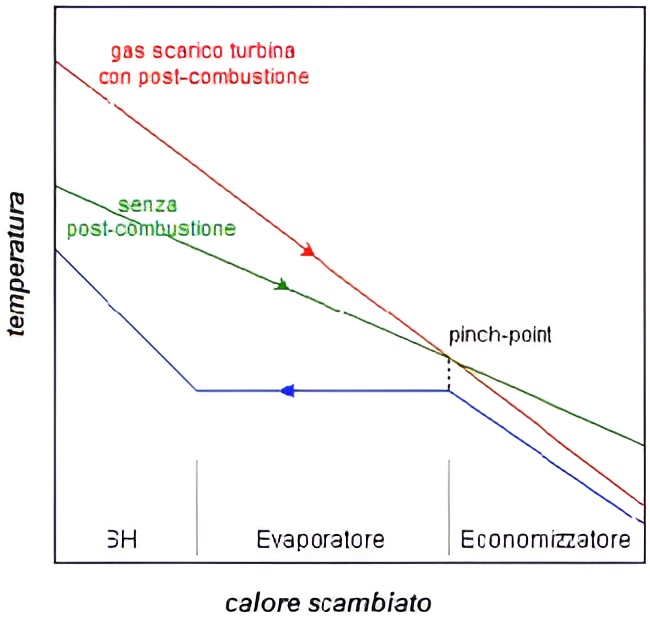
\includegraphics[width=0.5\linewidth]{immagini/impianticombinati13}
	\label{fig:impianticombinati13}
\end{figure}
	Al recupero di maggior calore corrisponde tuttavia una maggiore portata di combustibile, si definisce allora un rapporto sulla quantità di combustibile FPC come il calore del ciclo combinato post combusto diviso il calore del ciclo combinato con la sola combustione al turbogas
	\[FPC = \dfrac{Q_{CC,PC}}{Q_{CC,TG}}\]
	In modo che, il rendimento del ciclo combinato divenga
	\[\eta_{cc} = \dfrac{\eta_{TG} + (1-\eta_{TG}-\chi+FPC)\eta_I}{1+FPC}\]
\end{adjustwidth}

\subsection{Sistemi di Repowering}
\begin{adjustwidth}{2in}{}
	Col sistema di repowering si valorizza una turbina a vapore già preesistente.
	
	Si eliminano generalmente gli spillamenti ad alta pressione e di fa passare il circuito dell'acqua all'interno del GVR. 
	
	Questo sistema tuttavia cambia l'impianto perché ora la turbina - che era stata progettata per un certo numero di spillamenti - vede la sua portata variare: varia la componente $c_m$ dei triangoli di velocità, pertanto sarà necessario verificare se gli spillamenti si possono togliere senza compromettere irrimediabilmente la capacità di compiere lavoro utile della turbina. 
\end{adjustwidth}

\subsection{Sistemi di generazione aggiuntiva di vapore di media pressione}
\begin{adjustwidth}{2in}{}
	all'interno di un impianto a vapore, una pompa, che non è quella di alimento, si occupa di pompare parte dell'acqua proveniente dal degasatore in un circuito secondario all'interno del GVR di un sistema turbogas, col compito di generare vapore a pressione intermedia che verrà intercettato all'uscita dell secondo surriscaldamento, in modo da fornire all'impianto vapore una portata extra evolvente all'interno della turbina di bassa pressione.
\end{adjustwidth}




\subsection{Ricombustione in caldaia}
\begin{adjustwidth}{2in}{}
		I fumi in uscita dal gruppo turbogas vanno a sostituire l'aria in entrata del classico generatore di vapore, in questo modo, immettendo fumi già caldi, si risparmia sul combustibile e si garantisce una portata volumetrica maggiore.
\end{adjustwidth}

\subsection{Trasformazione del ciclo a vapore in un ciclo unfired}
\begin{adjustwidth}{2in}{}
	All'interno di un impianto a vapore si sostituisce il generatore di vapore con un GVR, questo produce più portata di vapore. 
\end{adjustwidth}	

\newpage
\part{Cicli inversi}
\begin{adjustwidth}{2in}{}
	L'effetto utile di un ciclo inverso, piuttosto che la produzione lavoro, è la produzione di un effetto frigorifero, ovvero la sottrazione di una potenza termica da un ambiente più freddo ad un ambiente più caldo "violando" il corso naturale degli eventi: ciò infatti è possibile solamente fornendo un'azione compensatrice sotto forma di energia, che può essere 
	\begin{itemize}
		\item \textbf{Meccanica}: macchine frigorifere a compressione di calore
		\item \textbf{Termica}: macchine frigorifere ad assorbimento
	\end{itemize}
	Tale ciclo può essere utilizzato sia per raffreddare che per riscaldare ambienti attraverso la pompa di calore. 		
\begin{figure}[H]
	\centering
	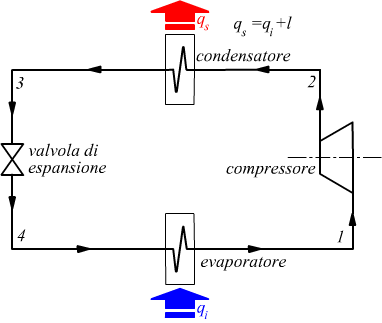
\includegraphics[width=0.4\linewidth]{immagini/cicliinversi}
	\label{fig:cicliinversi}
\end{figure}
	Il compressore è l'organo incaricato all'immissione del lavoro all'interno del ciclo, generalmente è di tipo volumetrico-alternativo, ciò significa all'entrata del compressore, per non danneggiare pistoni e cilindro, è necessario immettere vapore leggermente surriscaldato, perché nel caso ci fosse liquidi - per sua natura incomprimibile - si concentrerebbe sul volume morto e causerebbe problemi all'organo. 
	
	Il fluido esce dal compressore come vapore surriscaldato, dopodiché raggiunge il condensatore, questo è uno scambiatore di calore che si occupa di rilasciare calore verso l'ambiente. il fluido esce dal condensatore il condizioni di liquido saturo ed entra in una valvola di laminazione, che attraverso una trasformazione adiabatica di laminazione (isoentalpica), riporta il fluido alla pressione iniziale, a questo punto all'interno di un evaporatore assorbirà calore dall'ambiente e si ricondurrà nuovamente al compressore.
	
	Similmente agli impianti a vapore, poiché l'impianto è operativamente prossimo alle condizioni critiche, non si possono utilizzare le relazioni dei gas perfetti ma apposite tabelle dei liquidi refrigeranti. \newline 
	
	Sui diagrammi di interesse un ciclo frigorifero diviene 
\end{adjustwidth}		
\begin{figure}[H]
	\centering
	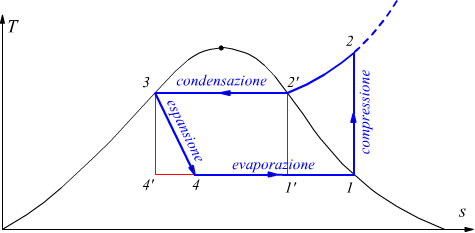
\includegraphics[width=0.4\linewidth]{immagini/cicliinversi1}
	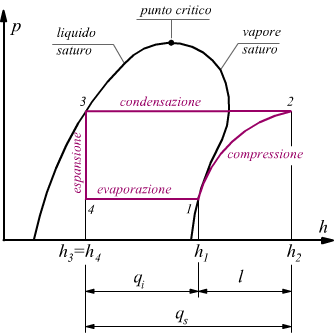
\includegraphics[width=0.4\linewidth]{immagini/cicliinversi2}
	\label{fig:cicliinversi1}
\end{figure}
\begin{adjustwidth}{2in}{}
	Come funziona un ciclo frigorifero? 
	
	La temperatura di passaggio di fase dipende dalla pressione,  comprimendo si alza la temperatura a cui avviene il passaggio di fase, per cui col compressore si porta la pressione superiore ad un livello tale per cui la temperatura di condensazione  sia almeno di 5 0 10 gradi superiore a quella esterna cosicché si possa condensare e quindi rilasciare calore all'ambiente esterno.
	
	Dopodiché espandendo all'interno della valvola di laminazione si ritorna alla pressione più bassa che corrisponde ad una temperatura di evaporazione di 5 o 10 gradi più bassa rispetto alla temperatura dell'ambiente da refrigerare. \newline 
	
	Nel caso in cui invece si utilizzasse questo sistema come pompa di calore l'effetto utile sarà dato dal condensatore, ovvero da quanta energia termica si riuscirà ad immettere nell'ambiente per riscaldarlo: rispetto al caso frigorifero si invertono così temperatura dell'utenza (ovvero quella dell'ambiente da condizionare, che ora è più alta) e la temperatura dell'ambiente esterno (che ora è più bassa) ma la macchina rimane la stessa e il ciclo rimane invariato, cambia soltanto l'effetto utile.\newline 
	
	Infatti per i cicli inversi, piuttosto che il rendimento si definisce il coefficiente di prestazione COP
	\[COP = \dfrac{\text{effetto utile}}{\text{energia spesa}}>1\]
	L'"efficienza" in questo tipo di cicli è maggiore dell'unità perché si sta convertendo lavoro (energia di prima specie, nobile, che può essere convertito in ogni forma di energia) in calore (energia di seconda specie, meno nobile).\newline 
	
	Per un ciclo frigorifero
	\[COP_f = \dfrac{Q_{41}}{L_{12}} = \dfrac{h_1-h_4}{h_2-h_1} = 2\div4\]
	Il range di valori è fortemente dipendente dalle condizioni operative, infatti tanto più cresce il $\Delta T$, tanto più si dovrà comprimere e tanto più il COP diminuirà.\newline 
	
	Per un ciclo pompa di calore 
	\[COP_{PdC} = \dfrac{Q_{23}}{L_{12}} = \dfrac{Q_{41} + L_{12} }{L_{12}} =COP_f + 1 = 3\div5\]
	
	Importante è la distinzione tra la temperatura dell'ambiente esterno $T_{amb}$ e la temperatura dell'utenza, ovvero quella dell'ambiente da condizionare $T_u$: il ciclo deve svolgersi sempre all'esterno di queste due temperature, l'evaporatore deve poter sempre assorbire calore ed il condensatore deve poter sempre cedere calore.
	
	Deve perciò esistere sempre un $\Delta T$ (lo stesso) tra la temperatura dell'ambiente e quella del condensatore e tra la temperatura dell'utenza e quella dell'evaporatore (Frigorifero); e tra la temperatura dell'ambiente e quella dell'evaporatore e tra la temperatura dell'utenza e del condensatore (Pompa di Calore).  
\end{adjustwidth}




\section{Variazione del ciclo base}
\subsection{Rigenerazione}
\begin{adjustwidth}{2in}{}
	
	DISEGNO
	
	Aggiungendo uno scambiatore intermedio che metta in contatto il fluido in uscita dal condensatore con quello in ingresso al compressore, si aggiungono 2 trasformazioni:
	\begin{itemize}
		\item \textbf{61} di preriscaldamento del vapore che andrà compresso
		\item \textbf{34} di raffreddamento del vapore che andrà laminato. 
		
		Queso in particolare giova al ciclo perché diminuendo il titolo del punto di inizio evaporazione (5) si aggiunge una parte di evaporazione in più e quindi sia aumenta l'effetto utile che è possibile trarre dal sistema. 
		\[COP = \dfrac{h_6-h_5}{h_2-h_1}\]
	\end{itemize} 
\end{adjustwidth}

\subsection{Interrefrigerazione}
\begin{adjustwidth}{2in}{}
	Per compiere un ciclo frigorifero com un grande $\Delta T$, dato che il lavoro di compressione sarebbe troppo elevato e sconveniente, si passa attraverso l'interrefrigerazione. 
	
	Si uniscono ciò due cicli a cascata mediante un serbatoio intermedio che raffredda il vapore che esce dal primo compressore e consente di frazionare la linea di espansione.
	
	DISEGNI
	
	La presenza del separatore intermedio consente di comprimere da 1 a 2 e raffreddare fino a 3 ripescando il vapore saturo e poi di ricomprimere fino a 4: ciò consente di risparmiare lavoro perché il punto di fine compressione, se questa non fosse stata frazionata, sarebbe stato in A.
	
	Un altro vantaggio è che alla pressione intermedia, tramite il separatore, si ripesca solamente liquido saturo in 7 e quindi si inizia ad evaporare al punto 8, se invece sia avesse espanso in una sola trasformazione a partire a 5, il punto di inizio evaporazione sarebbe stato B, e dato che $x_B>x_8$ con un effetto utile più ristretto. 
	
	In sostante il ciclo interrefrigerato porta con se du vantaggi: sulla compressione e sulla produzione di effetto utile. \newline 
	
	Questo schema prevede poi che la portata che fluisce nella zona superiore sia diversa da quella che fluisce nella zona inferiore, perché avvenendo in 6 la separazione, significa che nel punto 7 si prende solamente il liquido all'interno del separatore. 
	
	Come si determina il rapporto tra le due portate? Attraverso il bilancio termico al separatore
	\[\dot{m}_{cond}h_6 + \dot{m}_{evap}h_2 = \dot{m}_{cond}h_3 + \dot{m}_{evap}h_3 \]
	Allora 
	\[\Phi = \dfrac{\dot{m}_{cond}}{\dot{m}_{evap}} = \dfrac{h_2-h_7}{h_5-h_6}\]
	La potenza all'evaporatore sarà così calcolabile come 
	\[P_{evap} = \dot{m}_{evap}(h_1-h_8)\]
	Ed il COP sarà conseguentemente pari a 
	\[COP = \dfrac{Q_81}{L_{12}+L_{34}} = \dfrac{\dot{m}_{evap}(h_1-h_8)}{\dot{m}_{evap}(h_2-h_1) + \dot{m}_{cond}(h_4-h_3)} = \dfrac{h_1-h_8}{h_2-h_1 + \Phi(h_4-h_3)}\]
	Con questi tipi di impianti si può arrivare anche a $\Delta T \approx 60\degree C$.
\end{adjustwidth}





\section{Fluidi refrigeranti}
\begin{adjustwidth}{2in}{}
	Un fluido frigogeno dovrebbe avere
	\begin{itemize}
		\item \textbf{Alta temperatura critica}, al di sopra della temperatura di condensazione che si realizza nel ciclo. 
		\item \textbf{Bassa temperatura di solidificazione} in modo da non solidificare nelle normali condizioni di funzionamento
		\item \textbf{Alto calore di vaporizzazione} così da produrre un elevato effetto frigorifero
		\[P_{evap} = \dot{m}x\Delta h\]
		Crescendo $\Delta h$ - a potenza costante - diminuisce la portata e ciò consente di avere sezioni di passaggio più piccole e quindi macchine più compatte. 
		\item \textbf{Pressioni di esercizio} più \textbf{basse} possibili \textbf{ma superiori a quella atmosferica}, in questo modo oltre ad evitare costruzioni pesanti e costose si evitano infiltrazioni di aria nell'impianto
		\item \textbf{Chimicamente inerte}
		\item \textbf{Bassa potenzialità di distruzione dell'ozono e di effetto serra}
	\end{itemize}
	Tra i fluidi proposti possiamo individuare
	\begin{itemize}
		\item $H_2O$: inutilizzabile sotto gli 0 \degree C
		\item $CO_2, CH_3CH_2CH_3 (\text{propano})$: dalle caratteristiche termodinamiche poco convincenti
		\item $NH_3$: esplosivo se miscelato con $O_2$
		\item \textbf{Fluidi frigoneni alogenati}\\
		Non tossici, non infiammabili, non corrosivi, dalle ottime proprietà termodinamiche. 
		
		Questi vengono prodotti in maniera sintetica attraverso la sostituzione di un idrogeno con un cloro o un fluoro. \newline 
		
		La nomenclatura segue questa regola 
		\[R-MNP = C_{M+1}H_{N-1}Cl_xF_p\]
		Il fluido più comune è l'R134 (o HFC-134a o 1,1,1,2-tetrafluoroetano) la cui formula sarà
		\[C_2H_2F_4\]
		Tra questi tipo di fluidi si possono trovare 
		\begin{itemize}
			\item \textbf{CFC}: clorofluorocarburi
			\item \textbf{HCFC}: idroclorofluorocarburi\\
			
			Entrambi sono responsabili del buco dell'ozono, il Cloro catalizza la trasformazione  $O_3 \rightarrow O_2$
			
			\item \textbf{HFC}: idrofluorocarburi
			\item \textbf{FC}: fluorocarbuti\\
			
			Tutte e quattro le tipologie, se disperse in atmosfera, contribuiscono all'effetto serra.
		\end{itemize}
	\end{itemize}
\end{adjustwidth}


\newpage


\section{Macchine frigorifere ad assorbimento}
\begin{adjustwidth}{2in}{}
	Un'altra forma di energia che si può usare in input al ciclo è quella termica: in questo modo nascono le macchine frigorifere ad assorbimento.
	
	DISEGNO
	
	Si sostituisce il compressore con un'altra linea d'impianto e la pompa (ex compressore) ora elabora liquido piuttosto che gas e quindi richiede un lavoro specifico minore. \newline 
	
	Il principio di funzionamento si basa sulla solubilità dei fluidi, ovvero esiste un liquido assorbitore ed un liquido frigorifero che si possono miscelare, entrare in soluzione.
	
	Nel generatore si fornisce una potenza termica ad elevata temperatura cosicché da questa soluzione evapori il fluido frigorifero in modo da convogliarlo nel resto dell'impianto affinché assolva le sue funzioni quindi passare verso il condensatore, alla valvola  e all'evaporatore, dopo di ciò il vapore di fluido frigorifero incontrerà nell'assorbitore la soluzione di liquido assorbente e liquido frigorifero scarica di liquido frigorifero, in uscita dal generatore, in modo che il fluido frigorifero rientri di nuovo in soluzione liberando una certa potenza termica; a questo punto attraverso una pompa si aumenta la pressione della soluzione che viene reinviata al generatore. 
	
	Poiché il generatore si trova tra i $100\div130$\degree C e l'assorbitore è a temperatura ambiente, si può inserire un recuperatore che riscaldi il fluido al generatore e raffreddi il fluido all'assorbitore, in questo modo si riduce l'energia spesa $Q_G$. \newline 
	
	Le principali coppie di fluidi utilizzate sono		
\begin{itemize}
		\item $H_2O$: assorbitore - $NH_3$: refrigerante
		\item $BrLi$: assorbitore - $H_2O$: refrigerante per $T_u>0\degree C$
\end{itemize}
	Si definiscono anche qui 
	\[COP_f = \dfrac{Q_E}{Q_G}\]
	\[COP_{PdC} = \dfrac{Q_C-Q_A}{Q_G} = \dfrac{Q_G-Q_A}{Q_G} = COP_f+1\]
	
	Questi impianti vengono definiti tritermici, perché sussistono tre livelli di temperatura
	\[T_G = 1--\div130\degree C ~~T_{amb}\approxeq T_{cond} \approxeq T_A ~~> T_{evap} \approx T_u \]
\end{adjustwidth}


\newpage


\subsection{Studio del processo ideale}
\begin{adjustwidth}{2in}{}
	Si suddivida il processo in due sottoprocessi attraverso l'utilizzo di pozzi termici, tra la temperatura ambiente, quella dell'utenza e quella del generatore.
	
	DISEGNO
	
	In prima istanza si immagini la presenza di una macchina motrice di Carnot che assorbe la potenza termica alla temperatura più elevata e produce lavoro rilasciando calore all'ambiente per mezzo dell'assorbitore.
	 
	Si immagini poi una seconda macchina frigorifera di Carnot che riceva in ingresso sia il lavoro prodotto dalla macchina motrice di Carnot, che il calore dell'evaporatore e rilasci calore all'ambiente per mezzo dell'assorbitore.
	
	Allora è possibile scrivere, per la macchina motrice di Carnot
	\[\eta^* = \dfrac{L}{Q_G} = 1 - \dfrac{T_A}{T_G} \Rightarrow L = Q_G\left(1-\dfrac{T_A}{T_G}\right)\]
	Mentre per la macchina frigorifera di Carnot
	\[COP^* = \dfrac{Q_E}{L} = \dfrac{T_u}{T_A-T_u} \Rightarrow Q_E = L\dfrac{T_u}{T_A-T_u} = Q_G\dfrac{T_G-T_A}{T_G}\dfrac{T_u}{T_A-T_u} \]
	Allora il massimo COP aspirabile per una macchina reale sarà 
	\[COP_{\max} = \dfrac{Q_E}{Q_G} = \dfrac{T_G-T_A}{T_G}\dfrac{T_u}{T_A-T_u}\approx [1\div2]\]
	L'energia che ora si immette in ingresso è calore e non più lavoro: si sta convertendo energia di seconda specie in energia di seconda specie, il rendimento è sempre maggiore dell'unità ma minore del ciclo a compressione di vapore, se infatti si aumenta la nobilità dell'energia termica fornita aumentando la temperatura, ci si può avvicinare al rendimento del COP a vapore. \newline 
	
	I principali vantaggi che si possono sfruttare del ciclo ad assorbimento sono 
	\begin{itemize}
		\item Recupero di calore dispero dai processo industriali
		\item Piccoli impianti vicino all'utenza che recuperano il calore di scarto della grandi centrali termoelettriche (es. teleriscaldamento)
	\end{itemize}
\end{adjustwidth}


	

%DA DECOMMENTARE PER AVERE LA VERSIONE STAMPABILE A DUE PAGINE 	
%	\newpage
%		\null
%		\vfill
%\begin{tcolorbox}[height=4.5cm]
%	This box has a height of 4.5cm.
%\end{tcolorbox}
%		
	
\end{document}